%============================================================
% TEMPLATE PROYEK AKHIR — PENS
% Politeknik Elektronika Negeri Surabaya
% Berdasarkan Panduan Buku PA Sarjana Terapan A4 Rev05
%============================================================
% CARA PENGGUNAAN:
%   1. Buka config/variables.tex dan isi semua data Anda.
%   2. Tulis konten di folder chapters/ dan pages/.
%   3. Compile file ini (main.tex) dengan pdflatex + bibtex.
%============================================================

\documentclass[12pt, a4paper, twoside, openright, fleqn]{report}

% ── Konfigurasi (urutan penting: variables → packages → formatting) ──
%============================================================
% VARIABEL IDENTITAS DOKUMEN
%============================================================

% ── Identitas Mahasiswa ──────────────────────────────────────
\newcommand{\NamaMahasiswa}{Fernando Michael Panjaitan}
\newcommand{\NRP}{3122600051}

% ── Judul Proyek Akhir ───────────────────────────────────────
\newcommand{\JudulPA}{Fraud Detection dalam Data Perawatan Kesehatan melalui Metode Machine Learning}

% ── Dosen Pembimbing (sertakan gelar akademis) ───────────────
\newcommand{\NamaPembimbingSatu}{Rosiyah Faradisa, S.Si., M.Si.}
\newcommand{\NIPPembimbingSatu}{198607032009122004}
\newcommand{\NamaPembimbingDua}{Tessy Badriyah, S.Kom., M.T., Ph.D.}
\newcommand{\NIPPembimbingDua}{197009142001122001}

% ── Dosen Penguji (sertakan gelar akademis) ──────────────────
\newcommand{\NamaPengujiSatu}{Nama Lengkap dan Gelar}
\newcommand{\NIPPengujiSatu}{xxxxxxxxxxxxxxx}
\newcommand{\NamaPengujiDua}{Nama Lengkap dan Gelar}
\newcommand{\NIPPengujiDua}{xxxxxxxxxxxxxxx}

% ── Pembimbing Opsional ──────────────────────────────────────
\newcommand{\NamaPembimbingTiga}{}
\newcommand{\NIPPembimbingTiga}{}
\newcommand{\NamaPembimbingIndustri}{}

% ── Ketua Program Studi ──────────────────────────────────────
\newcommand{\NamaKetuaProdi}{Nama Ketua Program Studi}
\newcommand{\NIPKetuaProdi}{xxxxxxxxxxxxxxx}

% ── Program Studi & Institusi ────────────────────────────────
\newcommand{\NamaProdi}{Teknik Informatika}
\newcommand{\NamaDepartemen}{Departemen Teknik Informatika dan Komputer}

% ── Gelar yang Diperoleh ─────────────────────────────────────
\newcommand{\GelarLulus}{Sarjana Terapan Komputer (S.Tr.Kom.)}

% ── Tahun Kelulusan ──────────────────────────────────────────
\newcommand{\TahunLulus}{2025}

% ── Tanggal Sidang ───────────────────────────────────────────
\newcommand{\TanggalSidang}{Surabaya, 25 April 2026}

\input{config/packages}
%============================================================
% FORMATTING
% Semua pengaturan tampilan dan layout dokumen.
% File ini di-input setelah packages.tex dan variables.tex.
%============================================================

% ── Warna Institusi ──────────────────────────────────────────
\definecolor{pensbiru}{RGB}{0, 47, 167}    % Biru PENS (#002FA7)
\definecolor{penskuning}{RGB}{255, 193, 7} % Kuning/emas garis cover

% ── Geometri Halaman (Mirror Margin) ─────────────────────────
\geometry{
  a4paper,
  top    = 3cm,
  bottom = 3cm,
  inner  = 4cm,  % Margin kiri pada halaman ganjil (sisi jilid)
  outer  = 3cm,  % Margin kanan pada halaman ganjil
  twoside
}

% ── Spasi Baris ──────────────────────────────────────────────
\onehalfspacing % Spasi 1,5 sesuai panduan

% ── Indentasi & Paragraf ─────────────────────────────────────
\setlength{\parindent}{1.27cm}
\setlength{\parskip}{0pt}

% ── Persamaan Matematika ─────────────────────────────────────
\setlength{\mathindent}{10mm}
\setlength{\abovedisplayskip}{-15pt}
\setlength{\belowdisplayskip}{0pt}
\setlength{\abovedisplayshortskip}{0pt}
\setlength{\belowdisplayshortskip}{0pt}

% Nomor persamaan dicetak tebal-miring
\makeatletter
\renewcommand{\tagform@}[1]{\maketag@@@{\bfseries\itshape(#1)\@@italiccorr}}
\makeatother

% ── Format Judul Bab ─────────────────────────────────────────
\titleformat{\chapter}[display]
{\centering\fontsize{14}{17}\bfseries}
{BAB \thechapter}
{0pt}
{}
\titlespacing*{\chapter}{0pt}{0pt}{18pt}

% ── Format Judul Subbab (Section) ────────────────────────────
\titleformat{\section}
{\fontsize{14}{17}\bfseries}
{\thesection}
{1em}
{}
\titlespacing*{\section}{0pt}{15pt}{3pt}

% ── Format Judul Sub-subbab (Subsection) ─────────────────────
\titleformat{\subsection}
{\fontsize{12}{14}\bfseries}
{\thesubsection}
{1em}
{}
\titlespacing*{\subsection}{0pt}{8pt}{3pt}

% ── Batas Penomoran dan Daftar Isi ───────────────────────────
% 0 = Chapter, 1 = Section, 2 = Subsection, 3 = Subsubsection
\setcounter{secnumdepth}{2}
\setcounter{tocdepth}{2}

% ── Format Judul Sub-sub-subbab (Subsubsection) ──────────────
\titleformat{\subsubsection}
{\fontsize{12}{14}\bfseries}
{}
{0pt}
{}
\titlespacing*{\subsubsection}{0pt}{3pt}{2pt}

% ── Caption Gambar ───────────────────────────────────────────
\captionsetup[figure]{
  labelfont     = {it},
  textfont      = {it},
  font          = {small},   % ~11pt dalam dokumen 12pt
  justification = centering,
  skip          = 6pt,
  name          = Gambar,
  labelsep      = space
}

% ── Caption Tabel ────────────────────────────────────────────
\captionsetup[table]{
  labelfont     = {it},
  textfont      = {it},
  font          = {small},
  justification = centering,
  skip          = 6pt,
  position      = above,
  name          = Tabel,
  labelsep      = space
}
\renewcommand{\tablename}{Tabel}

% ── Format Default Tabularray ────────────────────────────────
% Berlaku untuk semua lingkungan tblr dan longtblr
\SetTblrInner{
  hlines, vlines,                                             % Garis kotak otomatis
  row{1} = {bg=gray!20, font=\bfseries, halign=c},           % Header: abu-abu, bold, center
  rowhead = 1,                                               % Ulangi header jika tabel terpotong halaman
}

\SetTblrInner[longtblr]{
  hlines, vlines,
  row{1} = {bg=gray!20, font=\bfseries, halign=c},
  rowhead = 1,
}

% ── Kustomisasi Khusus longtblr ──────────────────────────────
% 1. Menyamakan format caption longtblr dengan tabel biasa (Italic, 11pt, rata tengah)
\DefTblrTemplate{caption-sep}{default}{\space}   % Mengganti titik dua (:) menjadi spasi
\SetTblrStyle{caption-tag}{font=\small\itshape}  % "Tabel 3.1" miring & 11pt
\SetTblrStyle{caption-text}{font=\small\itshape} % Judul caption miring & 11pt
\SetTblrStyle{caption-halign}{c}                 % Memaksa caption rata tengah

% Mematikan teks "Continued on next page" dan caption ulangan di halaman selanjutnya
\DefTblrTemplate{contfoot-text}{default}{} % Hapus "Continued on next page"
\DefTblrTemplate{conthead-text}{default}{} % Hapus "(Continued)"
\DefTblrTemplate{capcont}{default}{}       % Hapus judul tabel ulangan
\DefTblrTemplate{contfoot}{default}{}      % Hapus ruang kosong di bawah
\DefTblrTemplate{conthead}{default}{}      % Hapus ruang kosong di atas

% ── Penomoran Gambar/Tabel/Persamaan per Bab ─────────────────
% Contoh: Gambar 3.1, Tabel 4.2, Persamaan (3.1)
\renewcommand{\thefigure}{\thechapter.\arabic{figure}}
\renewcommand{\thetable}{\thechapter.\arabic{table}}
\renewcommand{\theequation}{\thechapter.\arabic{equation}}

% ── Header & Footer ──────────────────────────────────────────
\pagestyle{fancy}
\fancyhf{}
\fancyfoot[C]{\thepage}
\renewcommand{\headrulewidth}{0pt}

\fancypagestyle{plain}{
  \fancyhf{}
  \fancyfoot[C]{\thepage}
  \renewcommand{\headrulewidth}{0pt}
}

% ── Halaman Kosong ───────────────────────────────────────────
% Halaman kosong pada cetak bolak-balik diberi keterangan
\makeatletter
\def\cleardoublepage{%
  \clearpage
  \if@twoside
  \ifodd\c@page\else
  \hbox{}
  \vspace*{\fill}
  \begin{center}
    \textit{Halaman ini sengaja dikosongkan}
  \end{center}
  \vspace{\fill}
  \thispagestyle{fancy}
  \newpage
  \if@twocolumn\hbox{}\newpage\fi
  \fi
  \fi
}
\makeatother

% ── Lingkungan Kutipan Panjang (> 2 baris) ───────────────────
% Font 10pt, margin kanan-kiri masuk 10mm, ditulis miring
\newenvironment{kutipanpanjang}{%
  \begin{list}{}{%
      \setlength{\leftmargin}{10mm}
      \setlength{\rightmargin}{10mm}
      \setlength{\topsep}{6pt}
      \setlength{\itemsep}{0pt}
      \setlength{\parsep}{0pt}
    }
  \item\fontsize{10}{12}\selectfont\ignorespaces
  }{%
    \unskip
  \end{list}
}

% ── Hyperref ─────────────────────────────────────────────────
% Tautan hitam tanpa kotak berwarna
\hypersetup{
  colorlinks = true,
  linkcolor  = black,
  citecolor  = black,
  urlcolor   = black,
  pdftitle   = {\JudulPA},
  pdfauthor  = {\NamaMahasiswa}
}

% ── Nama Bahasa Indonesia ────────────────────────────────────
\renewcommand{\contentsname}{DAFTAR ISI}
\renewcommand{\listfigurename}{DAFTAR GAMBAR}
\renewcommand{\listtablename}{DAFTAR TABEL}
\renewcommand{\bibname}{DAFTAR PUSTAKA}
\renewcommand{\appendixname}{LAMPIRAN}
\renewcommand{\chaptername}{BAB}

% ── Judul Daftar Isi/Gambar/Tabel: 14pt, Bold, Center ────────
\renewcommand{\cfttoctitlefont}{\hfill\fontsize{14}{17}\bfseries\MakeUppercase}
\renewcommand{\cftaftertoctitle}{\hfill\null}

\renewcommand{\cftloftitlefont}{\hfill\fontsize{14}{17}\bfseries\MakeUppercase}
\renewcommand{\cftafterloftitle}{\hfill\null}

\renewcommand{\cftlottitlefont}{\hfill\fontsize{14}{17}\bfseries\MakeUppercase}
\renewcommand{\cftafterlottitle}{\hfill\null}

\setlength{\cftbeforetoctitleskip}{0pt}
\setlength{\cftbeforeloftitleskip}{0pt}
\setlength{\cftbeforelottitleskip}{0pt}
\setlength{\cftaftertoctitleskip}{12pt}
\setlength{\cftafterloftitleskip}{12pt}
\setlength{\cftafterlottitleskip}{12pt}

% ── Prefix "Gambar" dan "Tabel" di LOF/LOT ───────────────────
\renewcommand{\cftfigpresnum}{Gambar }
\renewcommand{\cfttabpresnum}{Tabel }
\addtolength{\cftfignumwidth}{3.5em}
\addtolength{\cfttabnumwidth}{2.5em}

% ── Titik-titik di Daftar Isi ────────────────────────────────
\renewcommand{\cftdotsep}{1.5} % Rapat (default 4.5)

% ── Spasi Konsisten di Daftar Isi ────────────────────────────
\setlength{\cftbeforechapskip}{0pt}
\setlength{\cftbeforesecskip}{0pt}
\setlength{\cftbeforesubsecskip}{0pt}
\setlength{\cftbeforefigskip}{0pt}
\setlength{\cftbeforetabskip}{0pt}

% ── Font Level Bab: Bold ─────────────────────────────────────
\renewcommand{\cftchapfont}{\bfseries}
\renewcommand{\cftchappagefont}{\bfseries}
\renewcommand{\cftchapleader}{\cftdotfill{\cftdotsep}} % Titik untuk bab

% ── Font Level Section: Normal ───────────────────────────────
\renewcommand{\cftsecfont}{\normalfont}
\renewcommand{\cftsecpagefont}{\normalfont}

% ── Prefix "BAB" di Daftar Isi ───────────────────────────────
\renewcommand{\cftchappresnum}{BAB }
\addtolength{\cftchapnumwidth}{2.5em}

% ── Jarak (Spasi) Atas/Bawah Gambar dan Tabel ────────────────
\setlength{\intextsep}{15pt}
\setlength{\textfloatsep}{15pt}

\setlength{\bibsep}{3pt}

%============================================================
\begin{document}
%============================================================

% ── Halaman Sampul & Judul ───────────────────────────────────
%============================================================
% HALAMAN SAMPUL (Cover Berwarna)
% Dimensi sesuai Panduan Rev05:
%   Logo     : lebar 3,5 cm
%   Header   : tinggi 5 cm (area putih)
%   Garis    : tebal 0,5 cm (warna emas)
%   Konten   : latar belakang biru PENS
%============================================================
\begin{titlepage}
  \newgeometry{top=0pt, bottom=0pt, left=0pt, right=0pt}
  \setlength{\fboxsep}{0pt}
  \pagecolor{pensbiru}

  % ── Bagian 1: Header Putih (tinggi 5 cm) ─────────────────────
  \noindent
  \colorbox{white}{%
    \begin{minipage}[c][5cm][c]{\textwidth}
      \hspace*{3cm}
      \begin{minipage}[c]{4cm}
        
\includegraphics[width=3.5cm, keepaspectratio]{logo_pens.png}
      \end{minipage}
      \hfill
      \begin{minipage}[c]{8cm}
        \raggedleft
        {\color{pensbiru}\fontsize{20}{24}\bfseries\selectfont PROYEK AKHIR}
      \end{minipage}
      \hspace*{3.5cm}
    \end{minipage}
  }\par\nointerlineskip

  % ── Bagian 2: Garis Emas (tinggi 0,5 cm) ─────────────────────
  \noindent
  \colorbox{penskuning}{%
    \makebox[\textwidth][l]{\rule{0pt}{0.5cm}}%
  }\par\nointerlineskip

  % ── Bagian 3: Konten Biru ─────────────────────────────────────
  \begin{center}
    \color{white}

    \vspace*{1.6cm}

    \begin{minipage}{\dimexpr\paperwidth-6cm\relax}
      \centering
      \fontsize{18}{20}\bfseries\selectfont\MakeUppercase{\JudulPA}
    \end{minipage}
    \par

    \vspace{1cm}

    % Identitas mahasiswa: 16pt, bold
    {\fontsize{16}{20}\bfseries\selectfont \NamaMahasiswa\par}
    {\fontsize{16}{20}\bfseries\selectfont NRP. \NRP\par}

    \vspace{0.8cm}

    % --- Di dalam blok "Dosen Pembimbing" ---
    {\fontsize{16}{20}\bfseries\selectfont DOSEN PEMBIMBING\par}
    \vspace{0.3cm}
    {\fontsize{16}{20}\selectfont \NamaPembimbingSatu\par}
    {\fontsize{16}{20}\selectfont NIP. \NIPPembimbingSatu\par}
    \vspace{0.3cm}
    {\fontsize{16}{20}\selectfont \NamaPembimbingDua\par}
    {\fontsize{16}{20}\selectfont NIP. \NIPPembimbingDua\par}

    % Logika Pembimbing ke-3 (Akademik)
    \ifcsvoid{NamaPembimbingTiga}{}{%
      \vspace{0.3cm}
      {\fontsize{16}{20}\selectfont \NamaPembimbingTiga\par}
      {\fontsize{16}{20}\selectfont NIP. \NIPPembimbingTiga\par}
    }

    % Logika Pembimbing Industri
    \ifcsvoid{NamaPembimbingIndustri}{}{%
      \vspace{0.8cm}
      {\fontsize{16}{20}\bfseries\selectfont PEMBIMBING INDUSTRI\par}
      \vspace{0.3cm}
      {\fontsize{16}{20}\selectfont \NamaPembimbingIndustri\par}
    }

    \vspace{1cm}

    % Program studi: 16pt, bold, kapital
    {\fontsize{16}{20}\bfseries\selectfont PROGRAM STUDI SARJANA TERAPAN\par}
    {\fontsize{16}{20}\bfseries\selectfont \MakeUppercase{\NamaProdi}\par}
    {\fontsize{16}{20}\bfseries\selectfont \MakeUppercase{\NamaDepartemen}\par}

    \vspace{0.5cm}

    % Institusi dan tahun: 16pt, bold, kapital
    {\fontsize{16}{20}\bfseries\selectfont POLITEKNIK ELEKTRONIKA NEGERI SURABAYA\par}
    {\fontsize{16}{20}\bfseries\selectfont \TahunLulus\par}

  \end{center}

  \restoregeometry
\end{titlepage}
\pagecolor{white}
%============================================================
% HALAMAN JUDUL DALAM
% Sama dengan cover tetapi tanpa warna (hitam-putih).
% "PROYEK AKHIR" rata kanan, sisanya rata tengah.
%============================================================
\newpage
\thispagestyle{empty}

% "PROYEK AKHIR" rata kanan
\begin{flushright}
  {\fontsize{20}{0}\bfseries\selectfont PROYEK AKHIR\par}
\end{flushright}

\vspace{1.5cm}

\begin{center}

  \begin{minipage}{1\textwidth}
    \centering
    \fontsize{18}{20}\bfseries\selectfont\MakeUppercase{\JudulPA}
  \end{minipage}
  \par

  \vspace{1.2cm}

  % Identitas mahasiswa: 16pt, bold
  {\fontsize{16}{20}\bfseries\selectfont \NamaMahasiswa\par}
  {\fontsize{16}{20}\bfseries\selectfont NRP. \NRP\par}

  \vspace{0.8cm}

  % --- Di dalam blok "Dosen Pembimbing" ---
  {\fontsize{16}{20}\bfseries\selectfont DOSEN PEMBIMBING\par}
  \vspace{0.3cm}
  {\fontsize{16}{20}\selectfont \NamaPembimbingSatu\par}
  {\fontsize{16}{20}\selectfont NIP. \NIPPembimbingSatu\par}
  \vspace{0.3cm}
  {\fontsize{16}{20}\selectfont \NamaPembimbingDua\par}
  {\fontsize{16}{20}\selectfont NIP. \NIPPembimbingDua\par}

  % Logika Pembimbing ke-3 (Akademik)
  \ifcsvoid{NamaPembimbingTiga}{}{%
    \vspace{0.3cm}
    {\fontsize{16}{20}\selectfont \NamaPembimbingTiga\par}
    {\fontsize{16}{20}\selectfont NIP. \NIPPembimbingTiga\par}
  }

  % Logika Pembimbing Industri
  \ifcsvoid{NamaPembimbingIndustri}{}{%
    \vspace{0.8cm}
    {\fontsize{16}{20}\bfseries\selectfont PEMBIMBING INDUSTRI\par}
    \vspace{0.3cm}
    {\fontsize{16}{20}\selectfont \NamaPembimbingIndustri\par}
  }

  \vspace{1cm}

  % Program studi: 16pt, bold, kapital
  {\fontsize{16}{20}\bfseries\selectfont PROGRAM STUDI SARJANA TERAPAN\par}
  {\fontsize{16}{20}\bfseries\selectfont \MakeUppercase{\NamaProdi}\par}
  {\fontsize{16}{20}\bfseries\selectfont \MakeUppercase{\NamaDepartemen}\par}

  \vspace{0.5cm}

  % Institusi dan tahun: 16pt, bold, kapital
  {\fontsize{16}{20}\bfseries\selectfont POLITEKNIK ELEKTRONIKA NEGERI SURABAYA\par}
  {\fontsize{16}{20}\bfseries\selectfont \TahunLulus\par}

\end{center}
%============================================================
% HALAMAN PENGESAHAN
% Watermark background otomatis untuk 1 atau lebih halaman.
%============================================================
\cleardoublepage
\pagestyle{empty} % Memastikan seluruh halaman pengesahan tanpa nomor/header

% 1. Nyalakan watermark secara otomatis mulai dari halaman ini
\AddToShipoutPictureBG{%
  \tikz[remember picture, overlay]
  \node[inner sep=0pt] at (current page.center){%
    
\includegraphics[width=\paperwidth, height=\paperheight]{background_pens_repeated.png}%
  };
}

\begin{center}
  {\fontsize{20}{0}\bfseries HALAMAN PENGESAHAN\par}
  \vspace{0.8cm}

  \begin{minipage}{1\textwidth}
    \centering
    \fontsize{18}{16}\bfseries\selectfont\MakeUppercase{\JudulPA}
  \end{minipage}
  \par

  \vspace{0.6cm}

  {\fontsize{14}{17}\selectfont Oleh:\par}
  \vspace{0.1cm}

  {\fontsize{14}{17}\bfseries
    \NamaMahasiswa\par
  NRP. \NRP\par}

  \vspace{0.6cm}

  \begin{spacing}{1}
    {\fontsize{14}{17}\bfseries
      Proyek Akhir ini digunakan sebagai salah satu syarat untuk\\
      memperoleh Gelar \GelarLulus\\
      di Politeknik Elektronika Negeri Surabaya\\
    \TahunLulus\par}
  \end{spacing}
\end{center}

\vspace{0.2cm}
\begin{center}
  {\fontsize{14}{17}\bfseries Disetujui oleh:}
\end{center}
\vspace{0.2cm}

% Daftar pembimbing dan penguji beserta kolom tanda tangan
\noindent
{\fontsize{14}{17}\selectfont
  \begin{tabular}{@{}l c l c@{}}
    Pembimbing 1 & : & \NamaPembimbingSatu   & (\hspace{2.5cm}) \\
    &   & NIP. \NIPPembimbingSatu & \\[3pt]
    Pembimbing 2 & : & \NamaPembimbingDua   & (\hspace{2.5cm}) \\
    &   & NIP. \NIPPembimbingDua & \\[3pt]

    % Baris kondisional Pembimbing 3 (Akademik)
    \ifcsvoid{NamaPembimbingTiga}{}{%
      Pembimbing 3 & : & \NamaPembimbingTiga   & (\hspace{2.5cm}) \\
      &   & NIP. \NIPPembimbingTiga & \\[3pt]
    }

    % Baris kondisional Pembimbing Industri
    \ifcsvoid{NamaPembimbingIndustri}{}{%
      Pembimbing Industri & : & \NamaPembimbingIndustri & (\hspace{2.5cm}) \\
      &   &                        & \\[3pt]
    }

    Penguji 1    & : & \NamaPengujiSatu     & (\hspace{2.5cm}) \\
    &   & NIP. \NIPPengujiSatu   & \\[3pt]
    Penguji 2    & : & \NamaPengujiDua      & (\hspace{2.5cm}) \\
    &   & NIP. \NIPPengujiDua    & \\
  \end{tabular}
}

\vspace{0.3cm}

% 2. Blok Mengetahui dibungkus dalam minipage
%    Jika ruang tidak cukup, SELURUH kotak ini akan pindah ke halaman 2.
\noindent
\begin{minipage}{\textwidth}
  \begin{center}
    {\fontsize{14}{17}\bfseries Mengetahui,}\par
    {\fontsize{14}{17}\selectfont
      Ketua Program Studi Sarjana Terapan \NamaProdi\par
    Politeknik Elektronika Negeri Surabaya}\par
    \vspace{1.5cm}
    {\fontsize{14}{17}\selectfont
      \underline{\NamaKetuaProdi}\par
    NIP. \NIPKetuaProdi\par}
  \end{center}
\end{minipage}

% 3. Paksa render halaman terakhir, lalu MATIKAN watermark agar tidak bocor
\clearpage
\ClearShipoutPictureBG

% ── Halaman Prelim (penomoran romawi kecil) ──────────────────
\cleardoublepage
\pagestyle{fancy}
\pagenumbering{roman}
\setcounter{page}{1}
\onehalfspacing

%============================================================
% HALAMAN PERNYATAAN ORISINALITAS  (halaman i)
%============================================================
\addcontentsline{toc}{chapter}{PERNYATAAN ORISINALITAS}
\thispagestyle{fancy}

\begin{center}
  {\fontsize{20}{10}\bfseries PERNYATAAN ORISINALITAS\par}
\end{center}
\vspace{1.5cm}

{\fontsize{12}{15}\selectfont
  \begin{spacing}{1.5}

    \noindent Dengan ini saya menyatakan bahwa bagian atau keseluruhan proyek akhir ini:

    \begin{enumerate}[label=\arabic*., leftmargin=*]
      \item Adalah hasil karya sendiri dan tidak mengandung unsur plagiat dari pihak lain,
      \item Tidak pernah diajukan untuk mendapatkan gelar akademis pada suatu Perguruan Tinggi,
      \item Tidak pernah dipublikasikan atau ditulis oleh pihak lain,
      \item Mencantumkan rujukan dan kutipan dengan jujur dan benar terhadap sumber referensi
        lain yang menunjang pembahasan pada proyek akhir ini.
    \end{enumerate}

    Apabila ditemukan bukti bahwa pernyataan saya di atas tidak benar, maka saya bersedia
    menerima sanksi sesuai dengan ketentuan yang berlaku di Politeknik Elektronika Negeri
    Surabaya.

  \end{spacing}

  \vspace{2.5cm}

  % Blok tanggal dan tanda tangan di sebelah kanan
  \hfill
  \begin{minipage}{6.5cm}
    \TanggalSidang\\[2cm]
    \underline{\bfseries \NamaMahasiswa}\\
    \bfseries NRP. \NRP
  \end{minipage}
}
%============================================================
% HALAMAN PERNYATAAN PENGALIHAN HAK CIPTA  (halaman ii)
%============================================================
\cleardoublepage
\addcontentsline{toc}{chapter}{PERNYATAAN PENGALIHAN HAK CIPTA}
\thispagestyle{fancy}

\begin{center}
  {\fontsize{20}{10}\bfseries PERNYATAAN PENGALIHAN HAK CIPTA\par}
\end{center}
\vspace{1.5cm}

\noindent Dengan ini, saya yang bertanda tangan di bawah ini:

\vspace{0.5cm}
\noindent
\begin{tabular}{@{}ll p{10cm} @{}}
  Nama              & : & \NamaMahasiswa \\
  NRP               & : & \NRP \\
  Judul Proyek Akhir & : & \JudulPA \\
  Tanggal           & : & \TanggalSidang \\
\end{tabular}
\vspace{0.5cm}

\noindent menyatakan bahwa saya selaku penulis (dan/atau mewakili seluruh penulis) secara
sadar dan sukarela mengalihkan hak cipta (\textit{copyright}) atas proyek akhir tersebut
kepada Politeknik Elektronika Negeri Surabaya.

\noindent Demikian pernyataan ini saya buat dengan sebenar-benarnya dan tanpa paksaan
dari pihak mana pun.

\vspace{2cm}
\begin{flushleft}
  Hormat saya,\\[1cm]

  % Tempel materai di sini sebelum mencetak
  [Materai]\\[1cm]

  \underline{\bfseries \NamaMahasiswa}
\end{flushleft}
%============================================================
% HALAMAN ABSTRAK
%============================================================
\cleardoublepage
\chapter*{ABSTRAK}
\addcontentsline{toc}{chapter}{ABSTRAK}
\thispagestyle{fancy}

Program Jaminan Kesehatan Nasional (JKN) menggunakan mekanisme pembayaran Indonesian Case-Based Groups (INA-CBG) pada fasilitas kesehatan rujukan tingkat lanjutan, sehingga nilai klaim sangat dipengaruhi oleh diagnosis, prosedur, tingkat keparahan, dan hasil grouping. Kondisi ini membuka risiko fraud atau upcoding yang dapat menimbulkan kerugian finansial dan memperberat proses verifikasi klaim. Permasalahan utama pada domain ini adalah sulitnya mengidentifikasi klaim berisiko secara cepat, terukur, dan dapat dijelaskan, terutama ketika label fraud aktual pada level klaim tidak tersedia.

Penelitian ini mengajukan pendekatan deteksi indikasi risiko fraud/upcoding berbasis machine learning dengan pendekatan claim-centric, yaitu menjadikan satu klaim sebagai unit analisis utama dan memperkaya klaim dengan informasi administratif, klinis, biaya, diagnosis sekunder, dan histori layanan. Untuk mengatasi keterbatasan label fraud aktual, penelitian ini membentuk target awal melalui pseudo-labeling berbasis Isolation Forest, kemudian membandingkan beberapa model supervised learning melalui benchmarking multi-model. Pipeline penelitian juga mencakup feature engineering, branch-based feature selection, threshold tuning, serta interpretabilitas global dan lokal.

Eksperimen dilakukan pada 1.699.219 klaim FKRTL yang telah diintegrasikan ke dalam dataset claim-centric. Hasil eksperimen menunjukkan bahwa konfigurasi terbaik diperoleh pada model XGBoost dengan branch VIF dan threshold 0,80, dengan ROC-AUC 0,999876, PR-AUC 0,996046, F1-score 0,952511, precision 0,913917, recall 0,994507, dan MCC 0,951883 terhadap target pseudo-label. Perlu dicatat bahwa seluruh metrik evaluasi pada penelitian ini dihitung terhadap pseudo-label sebagai target proksi, sehingga hasilnya tidak boleh ditafsirkan sebagai akurasi deteksi fraud aktual yang telah diverifikasi. Hasil interpretabilitas menunjukkan bahwa fitur biaya, tarif grouping, histori nonkapitasi, special CMG, dan rasio tarif merupakan faktor penting yang mendorong skor risiko. Dengan demikian, sistem yang dibangun berpotensi digunakan sebagai alat bantu analitis untuk memprioritaskan pemeriksaan klaim berisiko tinggi, bukan sebagai penetapan fraud final.

\vspace{1cm}
\noindent\textbf{Kata Kunci:} Fraud Detection, Upcoding, INA-CBG, Machine Learning, Claim-Centric

%============================================================
% HALAMAN ABSTRACT
%============================================================
\cleardoublepage
\chapter*{ABSTRACT}
\addcontentsline{toc}{chapter}{ABSTRACT}
\thispagestyle{fancy}

\textit{The National Health Insurance (JKN) program applies the Indonesian Case-Based Groups (INA-CBG) payment mechanism for advanced healthcare facilities, making claim values highly dependent on diagnoses, procedures, severity levels, and grouping outcomes. This condition creates a risk of fraud or upcoding, which may lead to financial loss and complicate claim verification. The main challenge in this domain is how to identify high-risk claims in a fast, measurable, and explainable manner, especially when actual fraud labels are unavailable at the claim level.}

\textit{This study proposes a machine-learning-based approach for detecting fraud/upcoding risk indications using a claim-centric strategy, where each claim is treated as the main unit of analysis and enriched with administrative, clinical, cost, secondary diagnosis, and service history information. To address the absence of actual fraud labels, the study constructs initial targets through pseudo-labeling with Isolation Forest, followed by supervised multi-model benchmarking. The proposed pipeline also includes feature engineering, branch-based feature selection, threshold tuning, and both global and local interpretability.}

\textit{Experiments were conducted on 1,699,219 integrated FKRTL claims. The best configuration was achieved by XGBoost with the VIF branch and a threshold of 0.80, yielding a ROC-AUC of 0.999876, PR-AUC of 0.996046, F1-score of 0.952511, precision of 0.913917, recall of 0.994507, and MCC of 0.951883 against the pseudo-label target. Interpretability analysis indicates that cost-related features, grouping tariff, non-capitation service history, special CMG, and tariff ratios are key drivers of the risk score. Therefore, the proposed system has strong potential to support claim verification by prioritizing high-risk claims rather than issuing final fraud judgments.}

\vspace{1cm}
\noindent\textbf{Keywords:} Fraud Detection, Upcoding, INA-CBG, Machine Learning, Claim-Centric

%============================================================
% HALAMAN KATA PENGANTAR
%============================================================
\cleardoublepage
\chapter*{KATA PENGANTAR}
\addcontentsline{toc}{chapter}{KATA PENGANTAR}
\thispagestyle{fancy}

Puji syukur penulis panjatkan ke hadirat Tuhan Yang Maha Esa karena atas rahmat dan penyertaan-Nya penulis dapat menyelesaikan buku Proyek Akhir yang berjudul ``Fraud Detection dalam Data Perawatan Kesehatan melalui Metode Machine Learning'' dengan baik.

Penyusunan buku Proyek Akhir ini dilakukan sebagai salah satu syarat untuk menyelesaikan pendidikan pada Program Studi Sarjana Terapan Teknik Informatika, Politeknik Elektronika Negeri Surabaya. Penelitian ini membahas pendekatan machine learning berbasis claim-centric untuk mendeteksi potensi fraud atau upcoding pada klaim JKN/BPJS dalam sistem INA-CBG, khususnya ketika label fraud aktual pada level klaim tidak tersedia.

Dalam proses penyusunan Proyek Akhir ini, penulis memperoleh banyak bantuan, arahan, dan dukungan dari berbagai pihak. Oleh karena itu, penulis menyampaikan terima kasih kepada:

\begin{enumerate}[label=\arabic*., leftmargin=*]
  \item Ibu Rosiyah Faradisa, S.Si., M.Si. selaku dosen pembimbing yang telah memberikan arahan, masukan, dan bimbingan selama proses penelitian dan penulisan.
  \item Ibu Tessy Badriyah, S.Kom., M.T., Ph.D. selaku dosen pembimbing yang telah memberikan dukungan ilmiah, koreksi, dan saran yang sangat berarti dalam penyempurnaan penelitian ini.
  \item Keluarga penulis yang selalu memberikan doa, dukungan, dan semangat selama proses pengerjaan Proyek Akhir.
  \item Teman-teman serta seluruh pihak yang telah membantu penulis, baik secara langsung maupun tidak langsung, dalam menyelesaikan penelitian ini.
\end{enumerate}

Penulis menyadari bahwa buku Proyek Akhir ini masih memiliki keterbatasan. Oleh karena itu, penulis sangat terbuka terhadap kritik dan saran yang membangun untuk pengembangan penelitian ini di masa mendatang.

Akhir kata, penulis berharap semoga buku Proyek Akhir ini dapat memberikan manfaat bagi pengembangan analitik data klaim kesehatan, khususnya sebagai dasar prioritisasi verifikasi klaim berisiko tinggi.

\vspace{1cm}
\begin{flushright}
Surabaya, 25 April 2026\\[1.5cm]
Penulis
\end{flushright}


% ── Daftar Isi, Gambar, Tabel ────────────────────────────────
\cleardoublepage
\tableofcontents

\cleardoublepage
\begingroup
\renewcommand*{\addvspace}[1]{} % Hapus spasi ekstra antar entri
\listoffigures
\endgroup
\addcontentsline{toc}{chapter}{DAFTAR GAMBAR}

\cleardoublepage
\begingroup
\renewcommand*{\addvspace}[1]{}
\listoftables
\endgroup
\addcontentsline{toc}{chapter}{DAFTAR TABEL}

% ── Isi Utama (penomoran Arab dimulai dari 1) ─────────────────
\cleardoublepage
\pagenumbering{arabic}
\setcounter{page}{1}

%============================================================
% BAB 1 — PENDAHULUAN
% Revisi pivot sedang: fraud detection sebagai konteks, keluaran model sebagai indikasi risiko/prioritas verifikasi.
%============================================================
\chapter{PENDAHULUAN}

\section{LATAR BELAKANG}

Program Jaminan Kesehatan Nasional (JKN) merupakan sistem jaminan sosial kesehatan yang bertujuan memperluas akses masyarakat terhadap layanan kesehatan. Pada fasilitas kesehatan rujukan tingkat lanjutan (FKRTL), pembayaran layanan dilakukan menggunakan sistem Indonesian Case-Based Groups (INA-CBG), yaitu sistem pembayaran berbasis kelompok kasus dalam penyelenggaraan JKN \citep{kemenkes2014,kemenkes2016}. Dalam sistem ini, nilai klaim tidak dihitung berdasarkan setiap tindakan secara terpisah, melainkan ditentukan melalui proses \textit{grouping} yang mempertimbangkan diagnosis, prosedur, karakteristik layanan, dan tingkat keparahan kasus \citep{kemenkes2016}.

Skala layanan JKN yang besar membuat proses verifikasi klaim membutuhkan dukungan mekanisme prioritisasi berbasis data. Hingga 30 November 2025, pemanfaatan layanan kesehatan JKN telah mencapai 664,3 juta kunjungan dengan total beban jaminan sebesar Rp172,6 triliun, sehingga pemeriksaan klaim perlu diarahkan pada klaim yang memiliki indikasi risiko lebih tinggi \citep{djsn2025monthly}. Besarnya volume layanan tersebut memperkuat kebutuhan terhadap pendekatan analitis yang dapat membantu menyaring klaim untuk pemeriksaan lebih lanjut.

Ketergantungan nilai klaim terhadap diagnosis, prosedur, \textit{severity level}, dan hasil \textit{grouping} membuat ketepatan dokumentasi serta pengkodean menjadi aspek penting. Dalam konteks ini, \textit{upcoding} dipahami sebagai perubahan atau penggunaan kode diagnosis maupun prosedur yang menghasilkan tarif lebih tinggi daripada kondisi yang seharusnya \citep{maryana2024}. Risiko tersebut berkaitan dengan struktur insentif sistem pembayaran berbasis kelompok kasus, karena perubahan tarif dapat memengaruhi perilaku pengkodean rumah sakit dan mendorong kecenderungan pengodean pada tingkat keparahan yang lebih tinggi \citep{chalkley2022,crespin2024}.

Dalam literatur asuransi kesehatan, \textit{fraud} dipahami sebagai tindakan penipuan, penyimpangan, atau misrepresentasi yang dilakukan untuk memperoleh manfaat yang tidak semestinya dari sistem pembiayaan kesehatan \citep{villegas2021,timofeyev2022}. Pada konteks JKN, potensi penyimpangan dapat muncul melalui manipulasi prosedur medis, pemalsuan dokumen, penggunaan identitas fiktif, upcoding, maupun moral hazard penyedia layanan \citep{nurlianti2025,muliarta2023,syafrawati2023}. Namun, anomali klaim atau upcoding tidak selalu dapat langsung disamakan dengan fraud aktual, karena penetapan fraud tetap memerlukan proses verifikasi, audit, dan penilaian pihak berwenang.

Dalam praktik pengendalian klaim, proses verifikasi berperan untuk menjaga kesesuaian klaim dengan kaidah koding, aspek klinis, dan administrasi. Panduan Manual Verifikasi Klaim INA-CBG menjelaskan bahwa perbedaan persepsi antara verifikator BPJS Kesehatan dan \textit{coder} fasilitas kesehatan masih menjadi salah satu permasalahan dalam penyelesaian klaim INA-CBG, sehingga verifikasi diperlukan untuk meminimalkan \textit{dispute claim} dari sisi koding, klinis, dan administrasi \citep{bpjs2018}. Karena volume dan kompleksitas data klaim tinggi, proses pemeriksaan manual perlu didukung oleh pendekatan berbasis data yang dapat membantu menyusun prioritas verifikasi.

Machine learning telah digunakan dalam berbagai penelitian untuk mendeteksi potensi fraud pada klaim asuransi kesehatan karena mampu mempelajari pola dari data dan mengidentifikasi indikasi penyimpangan yang tidak selalu mudah ditemukan melalui aturan manual \citep{nabrawi2023,hamid2024,curtis2025}. Meskipun demikian, penerapan machine learning pada data klaim kesehatan menghadapi tantangan utama, yaitu tidak selalu tersedianya label fraud aktual pada level klaim. Dalam kondisi tersebut, anomaly detection, semi-supervised learning, dan pseudo-labeling dapat digunakan untuk membentuk sinyal awal terhadap klaim yang memiliki pola berbeda dari mayoritas klaim lain \citep{shekhar2023,settipalli2023,meulemeester2025,bakker2025,lee2013}.

Selain kemampuan mendeteksi indikasi risiko, model pada domain klaim kesehatan juga perlu dapat dijelaskan. Auditor dan verifikator tidak hanya membutuhkan skor risiko, tetapi juga alasan mengapa suatu klaim diprioritaskan untuk diperiksa. Model prediksi fraud asuransi kesehatan perlu memperhatikan aspek ketahanan dan interpretabilitas agar hasilnya dapat dipahami oleh pengguna \citep{wang2025}. Teknik explainable artificial intelligence seperti SHAP dan LIME dapat digunakan untuk membantu menjelaskan kontribusi fitur terhadap prediksi model \citep{ribeiro2016,lundberg2017,salih2025}.

Berdasarkan uraian tersebut, penelitian ini berfokus pada deteksi potensi fraud atau upcoding pada klaim JKN/BPJS dalam sistem INA-CBG. Penelitian ini tidak diposisikan sebagai sistem penetapan fraud final, melainkan sebagai pendekatan analitis untuk mengidentifikasi indikasi risiko dan membantu prioritisasi verifikasi klaim. Celah yang menjadi perhatian penelitian ini adalah kebutuhan untuk membangun pipeline \textit{claim-centric} yang menempatkan satu klaim sebagai unit analisis utama, membentuk pseudo-label ketika label fraud aktual tidak tersedia, membandingkan beberapa model machine learning, melakukan \textit{threshold tuning}, serta menyediakan interpretabilitas global dan lokal.

\section{PERMASALAHAN}

Permasalahan utama dalam penelitian ini adalah bagaimana membangun pendekatan machine learning yang dapat membantu mengidentifikasi klaim JKN/BPJS dengan indikasi risiko \textit{fraud} atau \textit{upcoding} dalam sistem INA-CBG. Klaim INA-CBG terbentuk dari kombinasi informasi administratif, klinis, biaya, diagnosis, prosedur, \textit{severity level}, dan hasil \textit{grouping}, sehingga indikasi risiko tidak dapat dibaca hanya dari satu atribut klaim \citep{kemenkes2016}. Oleh karena itu, diperlukan representasi data yang mampu menempatkan setiap klaim sebagai unit analisis utama dan menggabungkan konteks yang relevan di sekitar klaim tersebut.

Permasalahan berikutnya adalah tidak tersedianya \textit{ground-truth fraud label} pada level klaim dalam data yang digunakan. Ketiadaan label ini membuat \textit{supervised learning} tidak dapat langsung diterapkan sebagai \textit{fraud classifier} final. Pada kondisi keterbatasan label, pendekatan deteksi anomali, \textit{unsupervised learning}, dan \textit{semi-supervised learning} sering digunakan untuk membentuk sinyal awal terhadap observasi yang berpotensi menyimpang dari pola umum data \citep{shekhar2023,settipalli2023,meulemeester2025,bakker2025}. Dalam penelitian ini, sinyal awal tersebut digunakan sebagai pseudo-label atau label proksi, bukan sebagai bukti \textit{fraud} aktual.

Selain itu, proses verifikasi klaim membutuhkan mekanisme prioritisasi agar pemeriksaan dapat lebih terarah pada klaim yang memiliki indikasi risiko lebih tinggi. Dalam konteks \textit{fraud} dan anomaly detection, hasil model perlu dipahami sebagai alat bantu analitis yang mendukung proses pemeriksaan, bukan sebagai pengganti auditor atau verifikator. Oleh karena itu, penelitian ini perlu menggabungkan pemodelan prediktif, pengaturan ambang keputusan, dan interpretabilitas agar hasil model dapat digunakan untuk mendukung triase klaim secara lebih transparan \citep{wang2025,ribeiro2016,lundberg2017,salih2025}.

Berdasarkan uraian tersebut, rumusan masalah dalam penelitian ini adalah sebagai berikut:

\begin{enumerate}[label=\arabic*., leftmargin=*]
  \item Bagaimana mengintegrasikan data klaim JKN/BPJS ke dalam representasi \textit{claim-centric} sehingga setiap observasi merepresentasikan satu klaim FKRTL yang memuat konteks administratif, klinis, biaya, dan histori layanan?
  \item Bagaimana membentuk pseudo-label sebagai sinyal risiko awal ketika label \textit{fraud} aktual pada level klaim tidak tersedia?
  \item Bagaimana menerapkan dan membandingkan beberapa model machine learning untuk mempelajari pola klaim berisiko berdasarkan pseudo-label, tanpa mengklaim model sebagai penentu \textit{fraud} final?
  \item Bagaimana menentukan ambang keputusan yang sesuai agar keluaran model dapat digunakan untuk prioritas verifikasi klaim, bukan sekadar klasifikasi biner?
  \item Bagaimana menjelaskan faktor-faktor yang memengaruhi prediksi model sehingga hasil deteksi indikasi risiko dapat dipahami dan ditelusuri oleh pengguna?
\end{enumerate}

\section{BATASAN MASALAH}

Batasan masalah dalam penelitian ini adalah sebagai berikut:

\begin{enumerate}[label=\arabic*., leftmargin=*]
  \item Penelitian berfokus pada deteksi indikasi risiko \textit{fraud} atau \textit{upcoding} pada klaim JKN/BPJS dalam sistem INA-CBG, khususnya pada konteks klaim FKRTL.
  \item Unit analisis utama dalam penelitian ini adalah klaim. Setiap baris data diperlakukan sebagai satu klaim yang memuat informasi administratif, klinis, biaya, diagnosis, prosedur, serta histori layanan yang relevan.
  \item Penelitian tidak menggunakan label \textit{fraud} resmi hasil audit sebagai \textit{ground-truth}. Karena label \textit{fraud} aktual pada level klaim tidak tersedia, penelitian menggunakan pseudo-label berbasis anomaly detection sebagai target awal pemodelan. Pendekatan seperti ini relevan pada kondisi keterbatasan label, terutama ketika model perlu mengenali pola anomali atau risiko awal dari data klaim \citep{shekhar2023,meulemeester2025,bakker2025}.
  \item Pseudo-label yang dibentuk dalam penelitian ini tidak diartikan sebagai bukti \textit{fraud}, melainkan sebagai label proksi yang menunjukkan indikasi anomali atau risiko awal yang perlu ditinjau lebih lanjut.
  \item Model machine learning dalam penelitian ini diposisikan sebagai alat bantu analitis untuk prioritas verifikasi klaim, bukan sebagai sistem adjudikasi atau penetapan \textit{fraud} final.
  \item Evaluasi performa model dilakukan terhadap pseudo-label atau target indikatif yang dibentuk dalam eksperimen. Oleh karena itu, metrik evaluasi tidak ditafsirkan sebagai kemampuan model membuktikan \textit{fraud} aktual, melainkan sebagai kemampuan model mempelajari dan memprioritaskan pola klaim berisiko berdasarkan label proksi.
  \item Penelitian mencakup integrasi data berbasis \textit{claim-centric}, pembentukan pseudo-label, benchmarking beberapa model \textit{supervised learning}, \textit{threshold tuning}, serta interpretabilitas model.
  \item Interpretabilitas model digunakan untuk membantu memahami faktor yang berkaitan dengan prioritas risiko, baik secara global maupun lokal. Interpretasi tersebut tidak dimaksudkan sebagai bukti kausal, penilaian klinis final, atau keputusan audit resmi. Penggunaan interpretabilitas pada model \textit{fraud} dan anomaly detection penting untuk membantu pengguna memahami dasar prediksi yang dihasilkan model \citep{wang2025,ribeiro2016,lundberg2017,salih2025}.
  \item Keputusan akhir mengenai kebenaran \textit{fraud} tetap berada pada proses verifikasi, audit, dan penilaian pihak yang berwenang.
\end{enumerate}

\section{TUJUAN}

Penelitian ini bertujuan mengembangkan pendekatan machine learning berbasis \textit{claim-centric} untuk mendeteksi indikasi risiko \textit{fraud} atau \textit{upcoding} pada klaim JKN/BPJS dalam sistem INA-CBG. Pendekatan ini diarahkan sebagai alat bantu prioritisasi verifikasi klaim, bukan sebagai sistem penentu \textit{fraud} final. Secara khusus, tujuan penelitian ini adalah sebagai berikut:

\begin{enumerate}[label=\arabic*., leftmargin=*]
  \item Mengintegrasikan data klaim dan data pendukung ke dalam representasi \textit{claim-centric} sehingga setiap observasi merepresentasikan satu klaim FKRTL yang siap digunakan untuk analisis risiko.
  \item Membentuk fitur yang merepresentasikan konteks klaim, meliputi informasi administratif, klinis, biaya, diagnosis, prosedur, \textit{severity level}, serta histori layanan.
  \item Membentuk pseudo-label berbasis anomaly detection sebagai sinyal risiko awal ketika label \textit{fraud} aktual pada level klaim tidak tersedia.
  \item Menerapkan dan membandingkan beberapa model machine learning untuk mempelajari pola klaim berisiko berdasarkan pseudo-label yang telah dibentuk.
  \item Menentukan konfigurasi model dan ambang keputusan yang dapat digunakan untuk memprioritaskan klaim dengan indikasi risiko lebih tinggi.
  \item Mengevaluasi performa model secara proporsional terhadap pseudo-label, dengan memperhatikan bahwa metrik evaluasi tidak merepresentasikan pembuktian \textit{fraud} aktual.
  \item Menyediakan interpretabilitas model melalui analisis fitur penting serta penjelasan global dan lokal agar faktor yang memengaruhi prediksi klaim berisiko dapat dipahami.
\end{enumerate}

\section{MANFAAT}

\subsection{Bagi BPJS Kesehatan dan Regulator}

Penelitian ini dapat memberikan gambaran pendekatan analitik untuk membantu memprioritaskan klaim yang memiliki indikasi risiko \textit{fraud} atau \textit{upcoding}. Hasil penelitian dapat digunakan sebagai referensi awal dalam pengembangan mekanisme screening klaim berbasis data, terutama ketika pemeriksaan manual perlu diarahkan pada klaim yang paling layak ditinjau lebih lanjut. Namun, keluaran model tetap perlu diposisikan sebagai dukungan analitis, bukan sebagai keputusan \textit{fraud} final.

\subsection{Bagi Auditor dan Verifikator Klaim}

Penelitian ini dapat membantu auditor dan verifikator dalam menyusun prioritas pemeriksaan klaim. Skor risiko, ambang keputusan, dan penjelasan faktor pendorong prediksi dapat menjadi bahan awal untuk menelaah klaim yang menunjukkan pola tidak wajar. Dengan demikian, model dapat berfungsi sebagai alat bantu triase audit yang mendukung efisiensi pemeriksaan tanpa menggantikan penilaian profesional.

\subsection{Bagi Fasilitas Kesehatan}

Penelitian ini dapat memberikan masukan bagi fasilitas kesehatan mengenai pentingnya kualitas dokumentasi medis, ketepatan pengkodean diagnosis dan prosedur, serta konsistensi data klaim. Analisis terhadap faktor risiko dapat membantu fasilitas kesehatan memahami pola klaim yang berpotensi menimbulkan perhatian dalam proses verifikasi.

\subsection{Bagi Pengembangan Ilmu Pengetahuan}

Penelitian ini memberikan kontribusi pada penerapan machine learning untuk analitik klaim kesehatan, khususnya dalam kondisi tidak tersedianya label \textit{fraud} aktual pada level klaim. Kontribusi ilmiah penelitian terletak pada penggunaan pendekatan \textit{claim-centric}, pseudo-labeling berbasis anomaly detection, benchmarking model \textit{supervised learning}, \textit{threshold tuning}, serta interpretabilitas untuk mendukung prioritisasi klaim berisiko.

\subsection{Bagi Penelitian Selanjutnya}

Penelitian ini dapat menjadi dasar bagi pengembangan studi lanjutan yang menggunakan label audit resmi, validasi pakar, data klinis yang lebih lengkap, atau integrasi langsung dengan sistem verifikasi klaim. Penelitian selanjutnya juga dapat mengembangkan pendekatan yang lebih adaptif terhadap perubahan pola klaim dan memperkuat validasi terhadap hasil prioritisasi risiko.

\section{SISTEMATIKA PENULISAN}

Laporan Proyek Akhir ini disusun ke dalam lima bab utama agar pembahasan dapat disajikan secara runtut dan terarah. Sistematika penulisan laporan ini adalah sebagai berikut.

\begin{description}[leftmargin=2.2cm, labelsep=0cm, itemsep=0.1cm]
  \item[{\makebox[2.2cm][l]{\textbf{Bab 1}}}] \textbf{Pendahuluan}\\
  Bab ini menjelaskan latar belakang, permasalahan, batasan masalah, tujuan, manfaat, dan sistematika penulisan. Pembahasan diarahkan untuk menjelaskan urgensi deteksi indikasi risiko fraud/upcoding pada klaim JKN/BPJS dalam sistem INA-CBG serta posisi penelitian sebagai alat bantu prioritisasi verifikasi klaim.

  \item[{\makebox[2.2cm][l]{\textbf{Bab 2}}}] \textbf{Kajian Pustaka}\\
  Bab ini membahas konsep dan penelitian terkait yang menjadi dasar penelitian, meliputi sistem klaim INA-CBG, fraud dan upcoding pada klaim kesehatan, machine learning untuk analitik klaim, anomaly detection, pseudo-labeling, evaluasi model, serta interpretabilitas.

  \item[{\makebox[2.2cm][l]{\textbf{Bab 3}}}] \textbf{Deskripsi Sistem}\\
  Bab ini menjelaskan rancangan solusi yang digunakan dalam penelitian, mulai dari integrasi data berbasis claim-centric, pembentukan fitur, pseudo-labeling, pemodelan supervised, pembandingan model, threshold tuning, hingga interpretabilitas hasil.

  \item[{\makebox[2.2cm][l]{\textbf{Bab 4}}}] \textbf{Eksperimen dan Analisis}\\
  Bab ini menyajikan pelaksanaan eksperimen, karakteristik data, hasil pembentukan pseudo-label, hasil benchmarking model, evaluasi model final, serta analisis interpretabilitas. Pembahasan hasil dilakukan secara proporsional dengan menempatkan metrik evaluasi sebagai ukuran performa terhadap pseudo-label, bukan sebagai pembuktian fraud aktual.

  \item[{\makebox[2.2cm][l]{\textbf{Bab 5}}}] \textbf{Penutup}\\
  Bab ini berisi kesimpulan dan saran. Kesimpulan menjawab tujuan penelitian berdasarkan hasil eksperimen, sedangkan saran berisi arahan pengembangan penelitian, terutama terkait validasi lanjutan, penggunaan label audit resmi, dan penguatan integrasi dengan proses verifikasi klaim.
\end{description}

%============================================================
% BAB 2 — hasil konversi awal dari DOCX lama
%============================================================
\chapter{KAJIAN PUSTAKA}

Bab ini menguraikan landasan konseptual dan teoretis yang digunakan sebagai dasar untuk membangun penelitian deteksi potensi \emph{fraud} atau \emph{upcoding} pada klaim JKN/BPJS dalam sistem INA-CBG. Pembahasan dimulai dari deskripsi problem domain pada sistem klaim kesehatan nasional, kemudian dilanjutkan dengan teori penunjang yang menjelaskan dasar analisis berbasis data, serta diakhiri dengan penelitian terkait untuk menempatkan posisi dan orisinalitas penelitian ini.

\section{DESKRIPSI PERMASALAHAN}\label{deskripsi-permasalahan}

Permasalahan utama dalam proyek akhir ini adalah bagaimana mendeteksi potensi \emph{fraud} atau \emph{upcoding} pada klaim JKN/BPJS dalam sistem INA-CBG secara lebih terstruktur, terukur, dan dapat dijelaskan. Pada domain klaim kesehatan, deteksi tidak dapat dipahami hanya sebagai klasifikasi teknis antara klaim normal dan klaim bermasalah, tetapi harus dilihat dalam konteks sistem pembayaran, proses pengkodean, verifikasi klaim, dan keterbatasan ketersediaan label \emph{fraud} aktual. Oleh karena itu, deskripsi permasalahan pada bagian ini menempatkan klaim kesehatan sebagai objek utama yang dianalisis, sekaligus menegaskan bahwa keluaran penelitian diarahkan untuk mendukung prioritas verifikasi, bukan untuk membuktikan \emph{fraud} aktual secara hukum atau administratif.

\subsection{JKN/BPJS, FKRTL, dan Mekanisme Klaim INA-CBG}\label{jknbpjs-fkrtl-dan-mekanisme-klaim-ina-cbg}

Program Jaminan Kesehatan Nasional merupakan skema pembiayaan kesehatan yang dikelola oleh BPJS Kesehatan untuk menjamin akses pelayanan kesehatan bagi peserta. Pada fasilitas kesehatan rujukan tingkat lanjutan, pengajuan klaim dilakukan melalui mekanisme \emph{Indonesian Case-Based Groups} atau INA-CBG, yaitu sistem pembayaran prospektif berbasis kelompok kasus yang menetapkan besaran pembayaran berdasarkan kombinasi diagnosis, prosedur, dan karakteristik klinis tertentu. Permenkes Nomor 27 Tahun 2014 menjelaskan bahwa sistem INA-CBG merupakan bagian dari penyelenggaraan \emph{casemix} dalam program JKN, sedangkan petunjuk teknis \emph{e-claim} menunjukkan bahwa proses klaim dibentuk melalui entri data administratif dan klinis, proses \emph{grouping}, finalisasi klaim, dan pengiriman data klaim ke sistem verifikasi \citep{kemenkes2014}, \citep{kemenkes2016}.

Dalam konteks penelitian ini, FKRTL menjadi lokasi yang sangat relevan karena pada level inilah nilai klaim sangat dipengaruhi oleh ketepatan dokumentasi diagnosis, prosedur, kelas perawatan, dan tingkat keparahan kasus. Dengan demikian, klaim di FKRTL bukan hanya catatan biaya, melainkan representasi interaksi antara kondisi pasien, keputusan klinis, pengkodean rekam medis, dan aturan pembayaran. Karakter inilah yang menjadikan data klaim JKN/BPJS pada FKRTL penting untuk dianalisis ketika tujuan penelitian diarahkan pada deteksi potensi \emph{fraud} atau \emph{upcoding}.

\subsection{\texorpdfstring{Diagnosis, Prosedur, \emph{Severity Level}, \emph{Grouping}, dan Tarif Klaim}{Diagnosis, Prosedur, Severity Level, Grouping, dan Tarif Klaim}}\label{diagnosis-prosedur-severity-level-grouping-dan-tarif-klaim}

Pada sistem INA-CBG, nilai klaim ditentukan melalui proses \emph{grouping} yang mempertimbangkan diagnosis utama, diagnosis sekunder, prosedur, jenis pelayanan, dan \emph{severity level}. Struktur ini menunjukkan bahwa perubahan pada data klinis dan administratif dapat memengaruhi kelompok kasus yang dihasilkan beserta tarif yang melekat padanya. Petunjuk teknis e-claim dan dokumen INA-CBG menunjukkan bahwa proses entri klaim tidak berhenti pada pencatatan penyakit, tetapi berujung pada pembentukan kode kasus dan tarif pembayaran yang menjadi dasar pengajuan klaim kepada BPJS Kesehatan \citep{kemenkes2016}.

Hubungan antara komponen klaim dan struktur tarif inilah yang membuat sistem pembayaran berbasis kelompok kasus memiliki konsekuensi insentif. Chalkley dkk. menunjukkan bahwa perubahan harga dalam sistem pembayaran \emph{diagnosis-related groups} di Indonesia berkaitan dengan perubahan perilaku \emph{coding} rumah sakit, meskipun besarannya terbatas \citep{chalkley2022}. Temuan tersebut penting karena memperlihatkan bahwa struktur pembayaran tidak netral terhadap perilaku pencatatan klinis. Crespin dkk. (2024) juga menegaskan bahwa sistem pembayaran berbasis diagnosis dapat mendorong pengodean pasien ke tingkat intensitas atau keparahan yang lebih tinggi \citep{crespin2024}. Oleh sebab itu, diagnosis, prosedur, \emph{severity level}, \emph{grouping}, dan tarif klaim harus dipahami sebagai rangkaian unsur yang saling terkait dalam membentuk risiko ketidakwajaran klaim.

\subsection{\texorpdfstring{\emph{Upcoding} sebagai Bagian dari \emph{Fraud} atau \emph{Abuse Provider}}{Upcoding sebagai Bagian dari Fraud atau Abuse Provider}}\label{upcoding-sebagai-bagian-dari-fraud-atau-abuse-provider}

Dalam literatur \emph{fraud} kesehatan, \emph{upcoding} dipahami sebagai praktik penggunaan kode diagnosis atau prosedur yang menghasilkan pembayaran lebih tinggi daripada yang seharusnya. Villegas-Ortega dkk. menempatkan praktik semacam ini dalam spektrum \emph{health insurance fraud} sebagai bentuk misrepresentasi untuk memperoleh manfaat yang tidak sah \citep{villegas2021}. Maryana dan Aspan menjelaskan bahwa upcoding terjadi ketika diagnosis atau prosedur diubah menjadi kode yang bertarif lebih tinggi daripada kondisi klinis sebenarnya \citep{maryana2024}. Dalam konteks JKN/BPJS, praktik tersebut relevan karena tarif INA-CBG sangat bergantung pada hasil \emph{grouping}, sehingga perubahan kode dapat berdampak langsung pada besaran klaim.

\emph{Upcoding} pada \emph{provider} juga dapat dibaca sebagai bagian dari \emph{moral hazard} atau \emph{abuse} dalam sistem pembiayaan kesehatan. Syafrawati dkk. menunjukkan bahwa \emph{moral hazard provider} dalam skema asuransi kesehatan sosial dapat muncul dalam bentuk \emph{upcoding}, \emph{readmission}, dan \emph{unnecessary admission} \citep{syafrawati2023}. Muliarta dkk. serta Nurlianti dkk. juga menegaskan bahwa \emph{fraud} dalam JKN mencakup berbagai bentuk manipulasi administratif dan klinis yang dapat merugikan sistem pembiayaan kesehatan \citep{nurlianti2025}, \citep{muliarta2023}. Dengan demikian, \emph{upcoding} tidak berdiri sendiri sebagai kesalahan teknis, tetapi perlu ditempatkan dalam konteks perilaku organisasi dan insentif finansial pada sistem klaim kesehatan.

\subsection{\texorpdfstring{\emph{Fraud} Aktual, \emph{Error Coding}, dan Indikasi Risiko}{Fraud Aktual, Error Coding, dan Indikasi Risiko}}\label{fraud-aktual-error-coding-dan-indikasi-risiko}

Salah satu tantangan utama dalam domain ini adalah membedakan antara \emph{fraud} aktual, \emph{error coding}, dan indikasi risiko. \emph{Fraud} aktual mensyaratkan unsur kesengajaan dan biasanya memerlukan verifikasi administratif, klinis, atau audit untuk dibuktikan. Sebaliknya, \emph{error coding} dapat terjadi karena ketidaktepatan dokumentasi, perbedaan interpretasi aturan, keterbatasan \emph{coder}, atau ketidaklengkapan rekam medis. Sugiarti dkk. menunjukkan bahwa ketidaktepatan kode diagnosis dan ketidaksesuaian \emph{clinical pathway} dapat menghasilkan tarif klaim yang lebih tinggi, tetapi \emph{upcoding} tidak selalu dapat langsung disebut \emph{fraud} apabila unsur kesengajaannya belum dapat dibuktikan \citep{sugiarti2021}.

Perbedaan tersebut memiliki implikasi metodologis yang penting. Model analitik yang dibangun dari data klaim hanya membaca pola administrasi, biaya, histori layanan, dan karakteristik klinis yang terekam di dalam data. Karena itu, keluaran model lebih tepat diposisikan sebagai indikasi risiko atau sinyal ketidakwajaran klaim, bukan sebagai penetapan \emph{fraud} aktual. Posisi ini konsisten dengan kebutuhan verifikasi klaim dalam praktik, di mana keputusan akhir tetap berada pada auditor, verifikator, dan proses pembuktian yang lebih formal.

\subsection{Keterbatasan Verifikasi Manual pada Volume Klaim Besar}\label{keterbatasan-verifikasi-manual-pada-volume-klaim-besar}

Verifikasi manual memegang peran penting dalam menjaga kesesuaian klaim terhadap aturan koding, aspek klinis, dan kelengkapan administrasi. Panduan verifikasi INA-CBG menunjukkan bahwa proses verifikasi dapat melibatkan perbedaan persepsi antara \emph{coder} fasilitas kesehatan dan verifikator BPJS Kesehatan, terutama ketika dokumen klinis, diagnosis, atau prosedur tidak sepenuhnya sejalan dengan hasil \emph{grouping} klaim \citep{bpjs2018}. Namun, pada saat volume klaim sangat besar dan variabel klaim semakin kompleks, pemeriksaan manual terhadap seluruh klaim menjadi tidak efisien apabila dilakukan tanpa bantuan analitik.

Skala data JKN/BPJS membuat keterbatasan tersebut semakin nyata. Data klaim memuat informasi administratif, diagnosis utama dan sekunder, prosedur, kelas perawatan, histori layanan, hingga komponen tarif yang perlu dibaca secara bersama. Dalam kondisi seperti ini, verifikasi manual membutuhkan mekanisme prioritisasi agar auditor dan verifikator dapat memusatkan perhatian pada klaim yang paling berisiko. Dengan kata lain, persoalan utamanya bukan sekadar menemukan seluruh klaim bermasalah secara otomatis, tetapi menyediakan alat bantu yang mampu menyaring dan mengurutkan klaim berdasarkan indikasi risiko.

\subsection{Kebutuhan Analitik Berbasis Data untuk Prioritas Verifikasi}\label{kebutuhan-analitik-berbasis-data-untuk-prioritas-verifikasi}

Kebutuhan terhadap analitik berbasis data muncul karena data klaim kesehatan bersifat besar, heterogen, dan menyimpan pola yang tidak selalu dapat ditangkap oleh aturan statis. Timofeyev dan Jakovljevic menekankan bahwa \emph{fraud} dan \emph{corruption} dalam \emph{healthcare} menimbulkan kerugian finansial yang besar serta memerlukan respons yang lebih sistematis \citep{timofeyev2022}. Najar dkk. juga menunjukkan bahwa penanganan \emph{medical fraud} dan \emph{abuse} semakin bergeser ke arah integrasi deteksi berbasis data, pencegahan, dan respons hukum \citep{najar2025}. Dalam konteks ini, \emph{machine learning} menjadi relevan bukan karena menggantikan verifikasi, tetapi karena mampu membantu membaca pola dari volume data yang besar dan menandai klaim dengan risiko lebih tinggi.

Atas dasar itu, \emph{problem} yang diangkat dalam penelitian ini dirumuskan sebagai kebutuhan untuk mendeteksi potensi \emph{fraud} atau \emph{upcoding} pada klaim JKN/BPJS secara \emph{claim-centric}, yaitu dengan menjadikan satu klaim sebagai unit analisis utama. Pendekatan ini dibutuhkan agar integrasi atribut peserta, diagnosis, histori layanan, komponen tarif, dan indikator klinis dapat dibaca secara terpadu. Dengan demikian, sistem yang dibangun diarahkan untuk menghasilkan prioritas verifikasi klaim berisiko tinggi secara terukur dan dapat dijelaskan, bukan untuk membuat vonis \emph{fraud} akhir.

\section{TEORI PENUNJANG}\label{teori-penunjang}

Teori penunjang pada penelitian ini disusun untuk menjelaskan dasar konseptual dari domain permasalahan sekaligus dasar metodologis dari solusi yang diusulkan. Pembahasan tidak diarahkan untuk menguraikan implementasi eksperimen secara rinci, melainkan untuk membangun pemahaman mengapa pendekatan \emph{claim-centric}, \emph{pseudo-labeling}, \emph{benchmarking multi-model}, \emph{threshold tuning}, dan interpretabilitas relevan digunakan pada deteksi potensi \emph{fraud} atau \emph{upcoding} dalam sistem klaim JKN/BPJS.

\subsection{\texorpdfstring{\emph{Fraud} Kesehatan dan \emph{Upcoding}}{Fraud Kesehatan dan Upcoding}}\label{fraud-kesehatan-dan-upcoding}

\emph{Fraud} kesehatan secara umum dipahami sebagai tindakan penipuan atau misrepresentasi yang disengaja untuk memperoleh manfaat atau pembayaran yang tidak sah dari sistem pembiayaan kesehatan. Villegas-Ortega dkk. menunjukkan bahwa \emph{fraud} asuransi kesehatan memiliki manifestasi yang beragam, melibatkan \emph{provider}, \emph{beneficiary}, maupun pihak asuransi, serta dipengaruhi oleh faktor regulasi, organisasi, dan perilaku \citep{villegas2021}. Dalam editorial tentang \emph{fraud and corruption in healthcare}, Timofeyev dan Jakovljevic juga menekankan bahwa \emph{fraud} harus dibedakan dari kesalahan yang tidak disengaja karena \emph{fraud} selalu mengandung unsur pelanggaran yang disengaja \citep{timofeyev2022}.

Dalam penelitian ini, bentuk \emph{fraud} atau \emph{abuse} yang menjadi fokus adalah \emph{upcoding}. Crespin dkk. memperlihatkan bahwa pada sistem pembayaran berbasis diagnosis, pengodean pasien ke tingkat intensitas tertinggi dapat meningkat seiring perubahan praktik \emph{coding} dan berpengaruh besar terhadap pembayaran rumah sakit \citep{crespin2024}. Maryana dan Aspan menjelaskan bahwa \emph{upcoding} terjadi ketika diagnosis atau tindakan dikodekan lebih tinggi daripada seharusnya, sehingga menghasilkan nilai klaim yang lebih besar \citep{maryana2024}. Dengan demikian, teori tentang \emph{fraud} kesehatan dan \emph{upcoding} menjadi dasar untuk memahami bahwa ketidakwajaran klaim tidak selalu muncul dari biaya tinggi semata, melainkan dari hubungan antara representasi klinis, aturan \emph{coding}, dan insentif pembayaran.

\subsection{Sistem Klaim JKN/BPJS dan INA-CBG}\label{sistem-klaim-jknbpjs-dan-ina-cbg}

Sistem INA-CBG merupakan mekanisme pembayaran prospektif yang membayar layanan berdasarkan kelompok kasus, bukan berdasarkan setiap tindakan secara terpisah. Permenkes Nomor 27 Tahun 2014 menjelaskan bahwa sistem ini menggunakan prinsip \emph{casemix} dengan pengelompokan diagnosis dan prosedur yang memiliki kemiripan klinis dan pola penggunaan sumber daya \citep{kemenkes2014}. Petunjuk teknis e-claim menjelaskan lebih lanjut bahwa pembentukan klaim berlangsung melalui entri data administratif dan klinis, proses \emph{grouping}, finalisasi, dan pengiriman klaim \citep{kemenkes2016}. Karena itu, kualitas data pada tahap entri dan \emph{coding} berpengaruh langsung terhadap hasil \emph{grouping} dan nilai pembayaran.

Pada level operasional, panduan verifikasi INA-CBG menunjukkan bahwa verifikasi klaim mencakup pemeriksaan administratif, klinis, dan koding \citep{bpjs2018}. Chalkley dkk. memberikan dasar empiris bahwa dalam konteks Indonesia, perubahan tarif dapat berkorelasi dengan perubahan perilaku \emph{coding} rumah sakit \citep{chalkley2022}. Temuan tersebut memperkuat pandangan bahwa sistem pembayaran berbasis kelompok kasus memiliki potensi menciptakan insentif diskresi dalam proses \emph{coding}. Oleh sebab itu, teori tentang JKN/BPJS dan INA-CBG pada penelitian ini tidak hanya menjelaskan sistem pembayarannya, tetapi juga menjelaskan mengapa struktur sistem tersebut relevan terhadap problem deteksi potensi \emph{upcoding}.

\subsection{\texorpdfstring{Data Klaim Kesehatan dan Pendekatan \emph{Claim-Centric}}{Data Klaim Kesehatan dan Pendekatan Claim-Centric}}\label{data-klaim-kesehatan-dan-pendekatan-claim-centric}

Data klaim kesehatan merupakan bentuk data administratif yang merekam interaksi antara peserta, \emph{provider}, diagnosis, prosedur, pelayanan, dan pembiayaan. Dalam penelitian \emph{fraud detection}, data semacam ini bernilai tinggi karena memuat sinyal yang berkaitan dengan pola biaya, utilisasi layanan, hubungan antar kode, serta histori perilaku. Kumaraswamy dkk. menegaskan bahwa \emph{healthcare claims} data dapat ditransformasikan menjadi himpunan fitur sekunder yang lebih informatif untuk mendukung deteksi \emph{fraud} \citep{kumaraswamy2022}. Hamid dkk. dan Nabrawi serta Alanazi juga menunjukkan bahwa data klaim dapat dimanfaatkan untuk membangun pendekatan \emph{data mining} dan \emph{machine learning} pada \emph{healthcare insurance fraud detection} \citep{nabrawi2023}, \citep{hamid2024}.

Pendekatan \emph{claim-centric} berarti satu klaim dijadikan unit observasi utama, lalu diperkaya dengan informasi lain yang relevan. Secara teoretis, pendekatan ini memungkinkan penelitian membaca risiko pada level transaksi klaim secara langsung, bukan pada agregat \emph{provider} atau agregat peserta. Bagi penelitian ini, konsep tersebut penting karena potensi \emph{upcoding} muncul pada klaim tertentu yang dibentuk oleh kombinasi diagnosis, prosedur, \emph{severity level}, tarif, dan histori layanan. Dengan menjadikan klaim sebagai pusat analisis, representasi risiko menjadi lebih dekat dengan objek verifikasi yang sesungguhnya.

\subsection{\texorpdfstring{\emph{Machine Learning} untuk Deteksi Potensi \emph{Fraud}/\emph{Upcoding}}{Machine Learning untuk Deteksi Potensi Fraud/Upcoding}}\label{machine-learning-untuk-deteksi-potensi-fraudupcoding}

\emph{Machine learning} adalah pendekatan komputasional yang memungkinkan sistem belajar dari data untuk mengenali pola, melakukan klasifikasi, atau memprediksi kejadian tertentu. Dalam konteks \emph{fraud detection}, \emph{machine learning} digunakan karena aturan statis sering kali tidak cukup untuk menangkap pola penyimpangan yang kompleks dan berubah. Curtis dkk. menunjukkan bahwa penelitian \emph{healthcare fraud detection} telah memanfaatkan berbagai keluarga \emph{classifier}, baik \emph{supervised}, \emph{unsupervised}, maupun \emph{semi-supervised}, untuk menangani karakter data klaim yang besar, heterogen, dan tidak seimbang \citep{curtis2025}.

Hamid dkk. menekankan bahwa \emph{healthcare insurance fraud detection} menghadapi tantangan dari skema \emph{fraud} yang berkembang, kualitas data yang bervariasi, kebutuhan deteksi yang andal, serta potensi \emph{false positive} yang tinggi \citep{hamid2024}. Nabrawi dan Alanazi juga menunjukkan bahwa model \emph{machine learning} pada \emph{claims} dapat membantu mengenali pola yang sulit ditemukan secara manual \citep{nabrawi2023}. Dalam penelitian ini, teori \emph{machine learning} diposisikan sebagai dasar umum yang menjelaskan mengapa pendekatan klasifikasi berbasis data dapat digunakan untuk membentuk prioritas verifikasi klaim berisiko.

\subsection{\texorpdfstring{\emph{Anomaly Detection}, \emph{Pseudo-Labeling}, dan \emph{Weak/Semi-Supervised Learning}}{Anomaly Detection, Pseudo-Labeling, dan Weak/Semi-Supervised Learning}}\label{anomaly-detection-pseudo-labeling-dan-weaksemi-supervised-learning}

Salah satu keterbatasan mendasar pada \emph{fraud detection} berbasis klaim adalah tidak tersedianya label \emph{fraud} aktual pada level transaksi. Dalam kondisi seperti ini, \emph{anomaly detection} menjadi relevan karena pendekatan tersebut tidak bergantung pada label final. Settipalli dan Gangadharan menunjukkan bahwa pendekatan \emph{unsupervised multivariate analysis} dapat digunakan untuk mendeteksi \emph{fraud} pada \emph{health insurance claims} \citep{settipalli2023}. Shekhar dkk. juga memperlihatkan bahwa \emph{unsupervised machine learning} dapat digunakan untuk \emph{health care fraud detection} sekaligus tetap memberikan penjelasan yang dapat dibaca \citep{shekhar2023}. Meulemeester dkk. lebih lanjut menekankan bahwa \emph{unsupervised anomaly detection} dapat dikembangkan secara \emph{explainable} agar hasilnya bermanfaat untuk investigasi dan audit \citep{meulemeester2025}.

Ketika tujuan penelitian tidak berhenti pada identifikasi anomali, tetapi berlanjut ke model klasifikasi, maka \emph{pseudo-labeling} menjadi strategi yang relevan. \emph{Pseudo-labeling} membentuk target awal dari sinyal anomali atau label lemah yang tersedia, lalu menggunakan target tersebut pada tahap \emph{supervised learning}. Yoon dkk. melalui kerangka SPADE menunjukkan bahwa \emph{semi-supervised anomaly detection} dapat menggunakan \emph{pseudo-labeler} untuk mengatasi keterbatasan label dan \emph{mismatch} distribusi antara data berlabel dan tidak berlabel \citep{yoon2022}. Bakker dkk. juga menunjukkan bahwa kombinasi \emph{pseudo-labeling} dan \emph{anomaly detection} dapat membantu menangani label \emph{scarcity} dalam \emph{billing healthcare} \citep{bakker2025}. Secara teoretis, pendekatan ini sesuai dengan kebutuhan penelitian ini, karena klaim berisiko harus dibentuk dari sinyal awal yang informatif sebelum dibandingkan lebih lanjut melalui model \emph{supervised}.

\subsection{\texorpdfstring{\emph{Feature Engineering} pada \emph{Healthcare Claims}}{Feature Engineering pada Healthcare Claims}}\label{feature-engineering-pada-healthcare-claims}

\emph{Feature engineering} merupakan proses membangun variabel turunan yang lebih representatif daripada atribut mentah agar model dapat menangkap pola yang relevan dengan masalah penelitian. Kumaraswamy dkk. menegaskan bahwa \emph{fraud detection} pada \emph{healthcare claims} sangat bergantung pada kemampuan mengubah data klaim yang heterogen menjadi fitur-fitur sekunder yang mencerminkan \emph{business heuristics}, relasi antar aktor, dan karakter populasi layanan \citep{kumaraswamy2022}. Dengan kata lain, kualitas \emph{feature engineering} sangat menentukan apakah sinyal \emph{fraud} atau \emph{upcoding} dapat muncul secara jelas pada data.

Dalam penelitian ini, teori \emph{feature engineering} penting karena potensi \emph{upcoding} tidak cukup dibaca dari satu variabel mentah seperti tarif atau lama rawat saja. Yang lebih relevan adalah hubungan antar komponen biaya, intensitas diagnosis sekunder, histori layanan, indikator \emph{special} CMG, dan rasio turunan yang memperlihatkan ketidakwajaran pola klaim. Wang dkk. menunjukkan bahwa pemilihan fitur, reduksi fitur, dan interpretasi terhadap fitur yang dominan dapat meningkatkan kualitas prediksi pada \emph{healthcare insurance fraud detection} \citep{wang2025}. Oleh karena itu, \emph{feature engineering} dipahami sebagai proses membangun sinyal risiko klaim yang lebih kaya, bukan sekadar menambah jumlah variabel.

\subsection{\texorpdfstring{\emph{Threshold Tuning} dan Evaluasi pada Data Tidak Seimbang}{Threshold Tuning dan Evaluasi pada Data Tidak Seimbang}}\label{threshold-tuning-dan-evaluasi-pada-data-tidak-seimbang}

\emph{Fraud detection} pada data klaim hampir selalu berhadapan dengan distribusi kelas yang tidak seimbang, karena jumlah klaim berisiko umumnya jauh lebih sedikit dibandingkan klaim normal. Pada kondisi seperti ini, evaluasi tidak cukup mengandalkan satu ukuran umum seperti akurasi. Curtis dkk. dan Hamid dkk. menunjukkan bahwa metrik seperti \emph{precision}, \emph{recall}, \emph{F1-score}, \emph{ROC-AUC}, dan \emph{PR-AUC} lebih relevan karena memberikan gambaran yang lebih tepat mengenai kemampuan model dalam menangkap kelas minoritas dan menjaga kualitas pemeringkatan risiko {[}15, 20{]}. Dalam penelitian ini, \emph{Matthews Correlation Coefficient} juga relevan karena mampu membaca kualitas klasifikasi secara lebih seimbang pada distribusi kelas yang tidak merata.

Selain metrik evaluasi, \emph{threshold tuning} merupakan komponen teoritis yang penting ketika model digunakan untuk prioritas verifikasi. \emph{Threshold} bawaan seperti 0,5 tidak selalu sesuai dengan kebutuhan operasional. Shen dan Kurshan menunjukkan bahwa pemilihan \emph{threshold} pada \emph{fraud alert system} perlu memperhitungkan keseimbangan antara kemampuan deteksi dan kapasitas pemrosesan \emph{alert} \citep{shen2020}. Secara konseptual, hal ini sejalan dengan penelitian ini, karena tujuan model adalah menandai klaim berisiko tinggi untuk diperiksa lebih lanjut, bukan membuat keputusan otomatis final. Oleh karena itu, \emph{threshold tuning} dipahami sebagai proses penyesuaian ambang keputusan model agar lebih sesuai dengan tujuan deteksi risiko pada domain klaim kesehatan.

\subsection{Interpretabilitas Model}\label{interpretabilitas-model}

Interpretabilitas model diperlukan agar keluaran \emph{machine learning} dapat dipahami oleh pengguna domain, khususnya auditor dan verifikator klaim. Pada konteks \emph{fraud detection}, model yang hanya menghasilkan skor tanpa alasan akan sulit dipakai sebagai dasar prioritas pemeriksaan. Salih dkk. menjelaskan bahwa SHAP dan LIME merupakan dua pendekatan yang banyak digunakan dalam \emph{explainable artificial intelligence} untuk memahami perilaku model yang kompleks \citep{salih2025}. SHAP cenderung kuat untuk membaca kontribusi fitur secara konsisten pada tingkat global maupun lokal, sedangkan LIME berguna untuk menjelaskan prediksi individual melalui aproksimasi lokal.

Pada \emph{domain healthcare fraud}, kebutuhan interpretabilitas juga telah ditegaskan oleh beberapa penelitian. Shekhar dkk. dan Meulemeester dkk. menunjukkan bahwa \emph{explainable fraud detection} dapat membantu menghubungkan skor risiko dengan pola yang dapat ditinjau kembali oleh investigator {[}16, 17{]}. Wang dkk. juga menggunakan kombinasi \emph{feature importance}, SHAP, \emph{partial dependence plot}, dan LIME untuk menjelaskan alasan prediksi \emph{fraud} pada data asuransi kesehatan \citep{wang2025}. Dengan demikian, teori interpretabilitas pada penelitian ini menjadi dasar untuk memahami mengapa hasil model harus dapat dibaca baik pada tingkat global, misalnya melalui \emph{feature importance}, SHAP, dan PDP, maupun pada tingkat klaim individual melalui \emph{local explanation} seperti LIME.

\section{PENELITIAN TERKAIT}\label{penelitian-terkait}

Penelitian terkait pada bagian ini dibahas secara komparatif untuk menunjukkan bagaimana studi sebelumnya memandang masalah \emph{fraud} kesehatan, bagaimana pendekatan analitik dibangun, dan di mana letak perbedaan penelitian ini. Ulasan disusun dalam empat klaster utama agar posisi penelitian dapat terlihat lebih jelas, yaitu studi tentang \emph{fraud} atau \emph{upcoding} pada sistem pembayaran berbasis diagnosis, studi fraud JKN di Indonesia, studi \emph{healthcare claims fraud detection} berbasis \emph{machine learning}, serta studi \emph{unsupervised}, \emph{pseudo-labeling}, dan \emph{explainable fraud detection}.

\subsection{\texorpdfstring{Penelitian \emph{Fraud/Upcoding} pada Sistem Pembayaran Berbasis Diagnosis}{Penelitian Fraud/Upcoding pada Sistem Pembayaran Berbasis Diagnosis}}\label{penelitian-fraudupcoding-pada-sistem-pembayaran-berbasis-diagnosis}

Studi pada kelompok ini menekankan bahwa sistem pembayaran berbasis diagnosis dapat menciptakan insentif untuk melakukan diskresi \emph{coding}. Chalkley dkk. menunjukkan bahwa pada sistem DRG di Indonesia terdapat hubungan positif antara perubahan tarif dan perubahan konsentrasi aktivitas berkode tertentu, yang mengindikasikan adanya perilaku \emph{coding} yang sensitif terhadap struktur harga \citep{chalkley2022}. Crespin dkk. memperlihatkan bahwa kenaikan \emph{coding intensity} pada sistem pembayaran berbasis diagnosis dapat berkontribusi besar terhadap pertumbuhan pembayaran rumah sakit. Maryana dan Aspan melengkapi diskusi ini dengan penjelasan yuridis bahwa \emph{upcoding} merupakan perubahan kode diagnosis atau prosedur ke tarif yang lebih tinggi daripada seharusnya \citep{maryana2024}.

Kontribusi kelompok studi ini terletak pada penegasan bahwa \emph{upcoding} bukan sekadar persoalan teknis \emph{coding}, tetapi berkaitan langsung dengan struktur insentif pada sistem pembayaran kesehatan. Namun, studi-studi tersebut umumnya belum membangun \emph{pipeline} analitik berbasis klaim yang terintegrasi sampai tahap pemodelan risiko. Penelitian ini berbeda karena tidak hanya menggunakan temuan tentang insentif \emph{coding} sebagai \emph{problem domain}, tetapi juga mengembangkan mekanisme deteksi berbasis \emph{data claim-centric} untuk mendukung prioritas verifikasi klaim JKN/BPJS.

\subsection{\texorpdfstring{Penelitian \emph{Fraud} JKN/Indonesia}{Penelitian Fraud JKN/Indonesia}}\label{penelitian-fraud-jknindonesia}

Penelitian \emph{fraud} JKN di Indonesia umumnya menyoroti bentuk-bentuk \emph{fraud}, \emph{moral hazard provider}, serta peran rekam medis dan verifikasi dalam menelusuri klaim yang bermasalah. Muliarta dkk. dan Nurlianti dkk. meninjau bahwa \emph{fraud} pada pelaksanaan JKN melibatkan berbagai bentuk penyimpangan dan merupakan persoalan serius dalam tata kelola pembiayaan kesehatan {[}7, 8{]}. Syafrawati dkk. menunjukkan bahwa \emph{moral hazard provider} dalam implementasi asuransi kesehatan sosial dapat muncul dalam bentuk \emph{upcoding} dan perilaku layanan lain yang menyimpang \citep{syafrawati2023}. Sugiarti dkk. menelusuri potensi \emph{fraud} melalui rekam medis dan menunjukkan bahwa ketidaktepatan kode diagnosis serta ketidaksesuaian \emph{clinical pathway} berpengaruh pada nilai klaim \citep{sugiarti2021}.

Kelompok studi ini sangat penting untuk memperkuat konteks lokal Indonesia, tetapi Meioritas masih berfokus pada kajian konseptual, tinjauan literatur, atau audit berbasis dokumen. Pendekatan tersebut memberikan pemahaman domain yang kuat, tetapi belum banyak yang mendorong integrasi data klaim multi-sumber dan pemodelan \emph{machine learning} pada level klaim individual. Di sinilah penelitian ini mengambil posisi yang berbeda, yaitu dengan memanfaatkan \emph{data claim-centric} sebagai objek analisis dan menghubungkannya dengan pendekatan \emph{machine learning} untuk menyusun prioritas verifikasi secara lebih sistematis.

\subsection{\texorpdfstring{Penelitian \emph{Healthcare Claims Fraud Detection} dengan \emph{Machine Learning}}{Penelitian Healthcare Claims Fraud Detection dengan Machine Learning}}\label{penelitian-healthcare-claims-fraud-detection-dengan-machine-learning}

Kelompok berikutnya terdiri atas penelitian yang memanfaatkan \emph{machine learning} untuk mendeteksi \emph{fraud} pada \emph{healthcare claims}. Hamid dkk. menggabungkan \emph{association rule mining} dan teknik \emph{unsupervised learning} untuk mendeteksi \emph{healthcare insurance fraud} \citep{hamid2024}. Nabrawi dan Alanazi menunjukkan bahwa \emph{model machine learning} dapat digunakan untuk meningkatkan deteksi klaim yang mencurigakan pada data asuransi kesehatan \citep{nabrawi2023}. Wang dkk. mengembangkan \emph{model ensemble} yang \emph{robust} dan \emph{interpretable} untuk prediksi \emph{healthcare insurance fraud} dengan dukungan \emph{feature selection} dan teknik interpretabilitas \citep{wang2025}. Curtis dkk. melalui \emph{review} \emph{classifier healthcare fraud detection} menegaskan bahwa berbagai keluarga model telah digunakan, tetapi tantangan penting tetap berkisar pada \emph{class imbalance}, interpretabilitas, kualitas fitur, dan generalisasi model \citep{curtis2025}.

Studi-studi ini menunjukkan bahwa \emph{machine learning} memiliki potensi kuat untuk membaca pola \emph{fraud claims}. Meskipun demikian, sebagian besar penelitian tersebut dibangun pada \emph{dataset} non-Indonesia dan tidak selalu beroperasi pada konteks JKN/BPJS dengan struktur INA-CBG. Selain itu, banyak penelitian telah memiliki \emph{label fraud} yang lebih siap pakai atau menggunakan \emph{setting} yang berbeda dari kondisi klaim JKN. Penelitian ini mengambil posisi berbeda dengan membangun deteksi potensi \emph{fraud} atau \emph{upcoding} pada klaim JKN/BPJS berbasis \emph{claim-centric}, lalu menentukan model final melalui \emph{benchmarking multi-model} secara empiris.

\subsection{\texorpdfstring{Penelitian \emph{Unsupervised}, \emph{Pseudo-Labeling}, dan \emph{Explainable Fraud Detection}}{Penelitian Unsupervised, Pseudo-Labeling, dan Explainable Fraud Detection}}\label{penelitian-unsupervised-pseudo-labeling-dan-explainable-fraud-detection}

Karena label \emph{fraud} aktual pada level klaim tidak selalu tersedia, beberapa penelitian memilih jalur \emph{unsupervised} atau \emph{semi-supervised}. Settipalli dan Gangadharan menggunakan pendekatan \emph{unsupervised multivariate analysis} untuk \emph{fraud detection} pada \emph{health insurance claims} \citep{settipalli2023}. Shekhar dkk. menunjukkan bahwa \emph{unsupervised machine learning} dapat digunakan untuk \emph{explainable healthcare fraud detection}, sedangkan Meulemeester dkk. menekankan pentingnya \emph{explainable unsupervised anomaly detection} untuk data \emph{insurance} {[}16, 17{]}. Yoon dkk. melalui SPADE memberikan dasar metodologis bahwa \emph{semi-supervised anomaly detection} dapat menggunakan \emph{pseudo-labeler} untuk mengatasi keterbatasan label dan \emph{mismatch} distribusi \citep{yoon2022}. Bakker dkk. menunjukkan bahwa \emph{pseudo-labeling} dapat digunakan dalam \emph{billing healthcare} yang mengalami label \emph{scarcity} \citep{bakker2025}. Sementara itu, Kumaraswamy dkk. memperlihatkan bahwa rekayasa fitur yang baik tetap menjadi prasyarat penting agar sinyal risiko dapat muncul secara bermakna \citep{kumaraswamy2022}.

Dari kelompok studi ini terlihat bahwa \emph{anomaly detection}, \emph{pseudo-labeling}, dan \emph{explainability} merupakan kombinasi yang semakin penting dalam deteksi \emph{fraud} berbasis data. Meskipun demikian, masih sedikit penelitian yang secara eksplisit menempatkan klaim JKN/BPJS dalam sistem INA-CBG sebagai unit analisis utama, lalu membangun alur lengkap dari \emph{claim-centric data preparation}, pembentukan \emph{pseudo-label}, \emph{benchmarking multi-model}, \emph{threshold tuning}, dan interpretabilitas global serta lokal. Dengan demikian, celah riset yang diisi oleh penelitian ini terletak pada penggabungan konteks lokal JKN/BPJS dengan \emph{pipeline} analitik \emph{claim-centric} yang utuh, terukur, dan dapat dijelaskan untuk mendukung prioritas verifikasi klaim berisiko tinggi.

Tabel 2.1 menunjukkan bahwa penelitian-penelitian sebelumnya telah memberikan kontribusi penting dalam memahami \emph{fraud} kesehatan, insentif \emph{upcoding}, \emph{fraud detection} berbasis \emph{machine learning}, serta \emph{anomaly detection} yang dapat dijelaskan. Studi-studi tersebut memperlihatkan bahwa problem \emph{fraud} pada layanan kesehatan tidak hanya berkaitan dengan tindakan curang yang bersifat administratif, tetapi juga berhubungan dengan struktur insentif pada sistem pembayaran, kualitas pengkodean diagnosis dan prosedur, serta karakteristik data klaim.

Namun demikian, masih terdapat beberapa celah yang penting. Sebagian besar penelitian masih menggunakan data non-Indonesia, beroperasi pada konteks sistem pembayaran yang berbeda dari JKN/BPJS dan INA-CBG, atau belum membangun alur analitik yang utuh mulai dari pembentukan sinyal risiko awal ketika \emph{label fraud} aktual tidak tersedia sampai penyediaan interpretabilitas hasil pada level klaim. Oleh karena itu, penelitian ini mengambil posisi yang berbeda dengan menempatkan klaim JKN/BPJS dalam sistem INA-CBG sebagai unit analisis utama, lalu membangun pendekatan \emph{claim-centric} yang mencakup \emph{pseudo-labeling}, \emph{benchmarking multi-model}, \emph{threshold tuning}, dan interpretabilitas untuk mendukung prioritas verifikasi klaim berisiko tinggi.

\phantomsection\label{_Toc228109609}{}Tabel 2. 1 Komparasi Penelitian Terkait Deteksi Fraud/Upcoding pada Klaim Kesehatan

\begin{longtable}[]{@{}
  >{\raggedright\arraybackslash}p{(\columnwidth - 14\tabcolsep) * \real{0.0419}}
  >{\raggedright\arraybackslash}p{(\columnwidth - 14\tabcolsep) * \real{0.0845}}
  >{\raggedright\arraybackslash}p{(\columnwidth - 14\tabcolsep) * \real{0.1267}}
  >{\raggedright\arraybackslash}p{(\columnwidth - 14\tabcolsep) * \real{0.1267}}
  >{\raggedright\arraybackslash}p{(\columnwidth - 14\tabcolsep) * \real{0.1795}}
  >{\raggedright\arraybackslash}p{(\columnwidth - 14\tabcolsep) * \real{0.1583}}
  >{\raggedright\arraybackslash}p{(\columnwidth - 14\tabcolsep) * \real{0.1574}}
  >{\raggedright\arraybackslash}p{(\columnwidth - 14\tabcolsep) * \real{0.1251}}@{}}
\toprule\noalign{}
\begin{minipage}[b]{\linewidth}\raggedright
\textbf{No}
\end{minipage} & \begin{minipage}[b]{\linewidth}\raggedright
\textbf{Peneliti (Tahun)}
\end{minipage} & \begin{minipage}[b]{\linewidth}\raggedright
\textbf{Konteks/Data}
\end{minipage} & \begin{minipage}[b]{\linewidth}\raggedright
\textbf{Fokus Utama}
\end{minipage} & \begin{minipage}[b]{\linewidth}\raggedright
\textbf{Pendekatan/Metode}
\end{minipage} & \begin{minipage}[b]{\linewidth}\raggedright
\textbf{Kontribusi Kunci}
\end{minipage} & \begin{minipage}[b]{\linewidth}\raggedright
\textbf{Kelebihan Utama}
\end{minipage} & \begin{minipage}[b]{\linewidth}\raggedright
\textbf{Keterbatasan/Pembeda}
\end{minipage} \\
\midrule\noalign{}
\endhead
\bottomrule\noalign{}
\endlastfoot
1 & Chalkley dkk. (2021) & Data JKN Indonesia, sistem pembayaran berbasis DRG/INA-CBG & Sensitivitas perilaku \emph{coding} rumah sakit terhadap perubahan tarif & Analisis empiris kebijakan pembayaran & Menunjukkan hubungan antara perubahan tarif dan perubahan perilaku \emph{coding} & Sangat relevan dengan konteks Indonesia dan insentif INA-CBG & Tidak membangun model deteksi klaim berisiko pada level klaim individual \\
2 & Crespin dkk. (2024) & \emph{Data discharge-level} rumah sakit pada sistem pembayaran berbasis diagnosis & \emph{Upcoding} pada tingkat intensitas/\emph{severity} tertinggi & Analisis kuantitatif perubahan \emph{coding intensity} & Menunjukkan bahwa peningkatan \emph{coding intensity} dapat berkontribusi besar terhadap pertumbuhan pembayaran & Memperkuat hubungan antara \emph{severity-based payment} dan insentif \emph{upcoding} & Bukan konteks JKN/BPJS dan tidak menawarkan \emph{pipeline machine learning claim-centric} \\
3 & Sugiarti dkk. (2022) & Rekam medis rumah sakit dalam konteks JKN & Penelusuran potensi \emph{fraud} melalui akurasi kode diagnosis dan \emph{clinical pathway} & Studi kuantitatif-kualitatif berbasis dokumen rekam medis & Menunjukkan bahwa ketidaktepatan kode dan \emph{clinical pathway} dapat memengaruhi tarif klaim & Relevan untuk membedakan \emph{upcoding}, \emph{error coding}, dan unsur kesengajaan & Berbasis audit dokumen, belum mengembangkan model analitik berbasis data klaim skala besar \\
4 & Hamid dkk. (2024) & \emph{Healthcare insurance claims} & Deteksi \emph{healthcare insurance fraud} & \emph{Data mining, association rule mining}, dan \emph{unsupervised learning} & Menunjukkan bahwa kombinasi teknik \emph{data mining} dapat mendukung deteksi \emph{fraud} pada \emph{claims data} & Relevan untuk \emph{fraud detection} berbasis data klaim & Tidak berfokus pada konteks JKN/INA-CBG dan tidak menekankan pendekatan \emph{claim-centric Indonesia} \\
5 & Kumaraswamy dkk. (2022) & \emph{Healthcare claims data} & \emph{Feature engineering} untuk \emph{fraud detection} & Rekayasa fitur berbasis \emph{claims} dan \emph{business heuristics} & Menunjukkan pentingnya transformasi \emph{claims data} menjadi fitur sekunder yang lebih informatif & Sangat kuat sebagai dasar teoritis \emph{feature engineering} pada \emph{claims} & Fokus utama pada \emph{feature engineering}, bukan \emph{pipeline} lengkap \emph{pseudo-labeling} sampai interpretabilitas \\
6 & Settipalli \& Gangadharan (2022) & \emph{Health insurance claims} & \emph{Fraud detection} tanpa label fraud aktual & \emph{Unsupervised multivariate analysis} & Menunjukkan bahwa \emph{claims fraud} dapat dideteksi dengan pendekatan \emph{unsupervised} & Relevan untuk dasar \emph{anomaly detection} pada \emph{claims} & Belum menggabungkan \emph{pseudo-labeling}, \emph{benchmarking multi-model}, dan interpretabilitas secara utuh \\
7 & Shekhar dkk. (2022) & \emph{Health care fraud data} & \emph{Explainable fraud detection} tanpa label siap pakai & \emph{Unsupervised machine learning} dan \emph{explainable fraud detection} & Menunjukkan bahwa \emph{fraud detection} dapat dilakukan secara \emph{unsupervised} tetapi tetap \emph{explainable} & Menghubungkan \emph{anomaly detection} dengan interpretabilitas & Bukan konteks JKN/BPJS dan tidak menempatkan klaim INA-CBG sebagai unit analisis utama \\
8 & Meulemeester dkk. (2025) & \emph{Healthcare insurance data} & \emph{Explainable unsupervised anomaly detection} & \emph{Unsupervised anomaly detection} dengan \emph{explainability} & Menunjukkan bahwa \emph{anomaly detection} dapat diarahkan untuk investigasi/audit & Kuat untuk mendukung \emph{explainable anomaly detection} pada insurance data & Tidak membahas konteks INA-CBG dan tidak membangun \emph{supervised benchmarking} setelah \emph{pseudo-labeling} \\
9 & Polak dkk. (2025) & Literatur \emph{healthcare fraud detection} & \emph{Review classifier machine learning} pada \emph{healthcare fraud detection} & \emph{Review} berbagai \emph{classifier supervised}, \emph{unsupervised}, dan \emph{semi-supervised} & Memetakan tantangan utama seperti \emph{class imbalance}, kualitas fitur, interpretabilitas, dan generalisasi & Cocok sebagai payung penelitian terkait ML pada \emph{healthcare fraud} & Bersifat \emph{review}, bukan implementasi pada data JKN/BPJS \\
10 & Yoon dkk. (2022) & \emph{Tabular and image anomaly detection} & \emph{Semi-supervised anomaly detection under distribution mismatch} & SPADE, \emph{pseudo-labeler}, \emph{ensemble one-class classifiers} & Menunjukkan bahwa \emph{pseudo-labeling} dapat membantu ketika label terbatas dan distribusi data tidak seragam & Kuat sebagai dasar metodologis \emph{pseudo-labeling}/\emph{semi-supervised learning} & Bukan studi \emph{healthcare claims} secara langsung \\
11 & Bakker dkk. (2025) & \emph{Mental healthcare provider billing} & \emph{Anomaly detection} pada \emph{billing} dengan \emph{label scarcity} & \emph{Hybrid deep learning, pseudo-labeling via Isolation Forest} dan \emph{Autoencoder} & Menunjukkan bahwa \emph{pseudo-labeling} dapat membantu pada \emph{billing healthcare} dengan label terbatas & Relevan untuk menjelaskan label \emph{scarcity} pada \emph{data billing} kesehatan & Domainnya mental \emph{healthcare billing} dan masih belum spesifik JKN/INA-CBG \\
12 & Penelitian ini (2026) & Klaim JKN/BPJS dalam sistem INA-CBG, unit analisis satu klaim FKRTL & Deteksi potensi \emph{fraud/upcoding} untuk prioritas verifikasi & \emph{Claim-centric data preparation}, \emph{pseudo-labeling}, \emph{branch-based feature selection}, \emph{supervised benchmarking}, \emph{threshold tuning}, dan interpretabilitas & Mengintegrasikan konteks lokal JKN/BPJS dengan \emph{pipeline} analitik \emph{claim-centric} yang utuh & Menghubungkan \emph{problem domain} INA-CBG dengan analitik risiko yang terukur dan dapat dijelaskan & Hasil model tetap diposisikan sebagai indikasi risiko dan prioritas verifikasi, bukan pembuktian \emph{fraud} aktual \\
\end{longtable}

\section*{}

Berdasarkan Tabel 2.1, penelitian-penelitian sebelumnya telah memberikan kontribusi penting dalam memahami fraud kesehatan, insentif upcoding, fraud detection berbasis machine learning, serta anomaly detection yang dapat dijelaskan. Studi-studi tersebut menunjukkan bahwa problem fraud pada layanan kesehatan tidak hanya berkaitan dengan tindakan curang yang bersifat administratif, tetapi juga berhubungan dengan struktur insentif pada sistem pembayaran, kualitas pengkodean diagnosis dan prosedur, serta karakteristik data klaim yang kompleks. Dengan demikian, kajian terdahulu memberikan landasan yang kuat bahwa deteksi potensi fraud/upcoding memang membutuhkan pendekatan berbasis data yang lebih sistematis.

Namun demikian, masih terdapat beberapa celah yang penting. Sebagian besar penelitian masih menggunakan data non-Indonesia, beroperasi pada konteks sistem pembayaran yang berbeda dari JKN/BPJS dan INA-CBG, atau belum membangun alur analitik yang utuh mulai dari pembentukan sinyal risiko awal ketika label fraud aktual tidak tersedia sampai penyediaan interpretabilitas hasil pada level klaim. Di sisi lain, studi-studi lokal Indonesia umumnya masih berfokus pada kajian konseptual, audit dokumen, atau pembahasan fraud dari sisi kebijakan dan verifikasi, sehingga belum banyak yang mengintegrasikan data klaim multi-sumber dan pemodelan machine learning pada level klaim individual.

Oleh karena itu, penelitian ini mengambil posisi yang berbeda dengan menempatkan klaim JKN/BPJS dalam sistem INA-CBG sebagai unit analisis utama, lalu membangun pendekatan claim-centric yang mencakup data preparation, pseudo-labeling, branch-based feature selection, benchmarking multi-model, threshold tuning, dan interpretabilitas global serta lokal. Posisi ini membuat penelitian tidak hanya menerapkan machine learning untuk klasifikasi, tetapi juga merancang mekanisme analitis yang lebih sesuai untuk mendukung prioritisasi verifikasi klaim berisiko tinggi. Dengan kata lain, kontribusi penelitian ini terletak pada penggabungan konteks lokal JKN/BPJS, struktur data berbasis klaim, dan kebutuhan interpretabilitas ke dalam satu alur analisis yang terukur dan dapat dijelaskan.

%============================================================
% BAB 3 — hasil konversi awal dari DOCX lama
%============================================================
\chapter{DESKRIPSI SISTEM}

Bab ini menjelaskan rancangan solusi yang diusulkan untuk mendeteksi potensi fraud atau upcoding pada data klaim kesehatan JKN/BPJS. Penyajian bab disusun mengikuti alur pipeline penelitian, yaitu dimulai dari pembentukan dataset claim-centric, dilanjutkan dengan pembentukan pseudo-label, benchmarking model supervised, penentuan threshold keputusan, dan diakhiri dengan evaluasi serta interpretabilitas hasil. Dengan susunan tersebut, pembaca diharapkan dapat memahami hubungan antara sumber data, tahapan analisis, dan keluaran sistem yang dihasilkan secara lebih runtut.

Perancangan sistem pada penelitian ini berlandaskan pada pendekatan berbasis klaim atau~\emph{claim-centric}, yaitu menjadikan satu klaim sebagai unit analisis utama. Dengan pendekatan tersebut, sistem tidak hanya memeriksa nilai biaya klaim secara terpisah, tetapi juga mengaitkannya dengan informasi kepesertaan, diagnosis sekunder, histori layanan, dan karakteristik klinis yang relevan. Rancangan ini dipilih agar proses deteksi tidak berhenti pada identifikasi anomali, tetapi juga mampu memberikan dasar analitis yang lebih kuat untuk menjelaskan mengapa suatu klaim diprediksi berisiko.

\section{DESKRIPSI SOLUSI}\label{deskripsi-solusi}

Solusi yang diajukan pada penelitian ini adalah sistem deteksi potensi \emph{fraud} atau \emph{upcoding} pada klaim kesehatan JKN/BPJS berbasis~\emph{machine learning}~dengan pendekatan~\emph{claim-centric}. Sistem ini dirancang untuk membantu proses identifikasi klaim yang memiliki tingkat risiko tinggi berdasarkan pola biaya, kondisi klinis, atribut peserta, dan riwayat layanan kesehatan yang tercatat pada data klaim. Fokus utama penelitian bukan untuk menetapkan bahwa suatu klaim terbukti \emph{fraud} secara hukum, melainkan untuk membangun mekanisme analitis yang mampu menandai klaim-klaim yang patut diprioritaskan untuk pemeriksaan lebih lanjut.

Pendekatan~\emph{claim-centric}~digunakan dengan menjadikan tabel~FKRTL~sebagai pusat analisis. Setiap baris data merepresentasikan satu klaim, kemudian diperkaya dengan informasi dari tabel lain, seperti data kepesertaan, diagnosis sekunder, serta histori layanan sebelumnya dari layanan FKTP dan nonkapitasi. Dengan rancangan ini, sistem dapat memandang klaim sebagai satu entitas yang utuh, bukan hanya sebagai catatan biaya, sehingga deteksi risiko dapat mempertimbangkan konteks administratif, klinis, dan historis secara bersamaan.

Untuk menangani keterbatasan utama berupa tidak tersedianya label \emph{fraud} transaksi riil pada level klaim, penelitian ini menggunakan pendekatan~\emph{hybrid fraud detection modeling}. Pada tahap awal, sistem menerapkan~\emph{Isolation Forest}~untuk melakukan~\emph{pseudo-labeling}~terhadap klaim yang memiliki pola anomali. Pseudo-label ini kemudian digunakan sebagai target pada tahap~\emph{supervised learning}~agar model dapat mempelajari pola yang membedakan klaim berisiko dan klaim normal. Pendekatan ini dipilih karena memungkinkan penelitian tetap membangun model prediktif meskipun tidak tersedia label \emph{fraud} final yang siap pakai.

Setelah \emph{pseudo-label} terbentuk, sistem melakukan~\emph{benchmarking}~terhadap beberapa model~\emph{supervised learning}~untuk memperoleh model dengan performa terbaik. Strategi ini digunakan agar pemilihan model tidak didasarkan pada asumsi awal terhadap satu algoritma tertentu, tetapi pada hasil evaluasi \emph{empiris} dari beberapa kandidat model. Dengan demikian, model final yang dipilih benar-benar merepresentasikan konfigurasi yang paling sesuai terhadap karakteristik data klaim yang digunakan dalam penelitian ini.

Selain menekankan performa prediksi, solusi yang diusulkan juga menempatkan interpretabilitas sebagai komponen penting. Interpretabilitas diperlukan agar hasil prediksi model tidak berhenti pada pemberian skor risiko, tetapi juga dapat dijelaskan melalui fitur-fitur yang berkontribusi terhadap keputusan model, baik pada tingkat global maupun lokal. Hal ini penting karena domain klaim kesehatan menuntut hasil analisis yang tidak hanya akurat, tetapi juga dapat dipahami dan dipertanggungjawabkan. Oleh sebab itu, sistem ini dirancang untuk menghasilkan deteksi potensi fraud yang terstruktur, terukur, dan dapat dijelaskan secara analitis.

\phantomsection\label{_Toc228109620}{}Tabel 3. 1 Komponen Utama Solusi yang Diusulkan

\begin{longtable}[]{@{}
  >{\raggedright\arraybackslash}p{(\columnwidth - 4\tabcolsep) * \real{0.2524}}
  >{\raggedright\arraybackslash}p{(\columnwidth - 4\tabcolsep) * \real{0.3411}}
  >{\raggedright\arraybackslash}p{(\columnwidth - 4\tabcolsep) * \real{0.4065}}@{}}
\toprule\noalign{}
\begin{minipage}[b]{\linewidth}\raggedright
\textbf{Komponen}
\end{minipage} & \begin{minipage}[b]{\linewidth}\raggedright
\textbf{Fungsi}
\end{minipage} & \begin{minipage}[b]{\linewidth}\raggedright
\textbf{Kontribusi dalam Sistem}
\end{minipage} \\
\midrule\noalign{}
\endhead
\bottomrule\noalign{}
\endlastfoot
\emph{Claim-centric integration} & Menjadikan klaim sebagai unit analisis utama & Menyatukan informasi klaim, peserta, diagnosis, dan histori layanan \\
\emph{Pseudo-labeling} & Membentuk label awal berbasis anomali & Mengatasi ketiadaan label \emph{fraud} transaksi riil \\
\emph{Supervised benchmarking} & Membandingkan beberapa model klasifikasi & Memilih model terbaik berdasarkan hasil evaluasi \\
\emph{Threshold tuning} & Menentukan ambang klasifikasi optimal & Menyesuaikan keputusan akhir model \\
\emph{Interpretability} & Menjelaskan hasil prediksi model & Mendukung pemahaman faktor risiko klaim \\
\end{longtable}

Tabel 3.1 merangkum komponen utama solusi yang diusulkan dalam penelitian ini. Setiap komponen memiliki peran yang saling terhubung, mulai dari pembentukan dataset berbasis klaim, pembentukan \emph{pseudo-label}, pemilihan model terbaik, hingga penjelasan terhadap hasil prediksi.

\section{\texorpdfstring{PERANCANGAN SISTEM}{PERANCANGAN SISTEM}}\label{perancangan-sistem}

Bagian ini menjelaskan desain sistem secara teknis dan runtut, mulai dari tahap persiapan data berbasis klaim, proses pemodelan deteksi fraud secara hybrid, hingga tahap evaluasi dan interpretabilitas hasil. Perancangan sistem disusun dalam bentuk alur bertahap agar hubungan antara data masukan, proses analisis, dan keluaran sistem dapat dipahami secara menyeluruh. Dengan rancangan ini, sistem tidak hanya berfungsi untuk menghasilkan prediksi risiko, tetapi juga menyediakan dasar analitis yang dapat digunakan untuk menjelaskan alasan di balik prediksi tersebut.

Secara umum, desain sistem pada penelitian ini terdiri atas tiga komponen utama, yaitu~\emph{Claim-Centric Data Preparation},~\emph{Hybrid Fraud Detection Modeling}, dan~\emph{Evaluation and Interpretability}. Komponen pertama berfokus pada penyiapan data mentah menjadi dataset analisis berbasis klaim. Komponen kedua berfokus pada pembentukan pseudo-label, pembandingan model, dan pemilihan model terbaik. Komponen ketiga berfokus pada evaluasi model final dan interpretasi hasil prediksi. Hubungan antar ketiga komponen tersebut ditunjukkan pada Gambar 3.1.

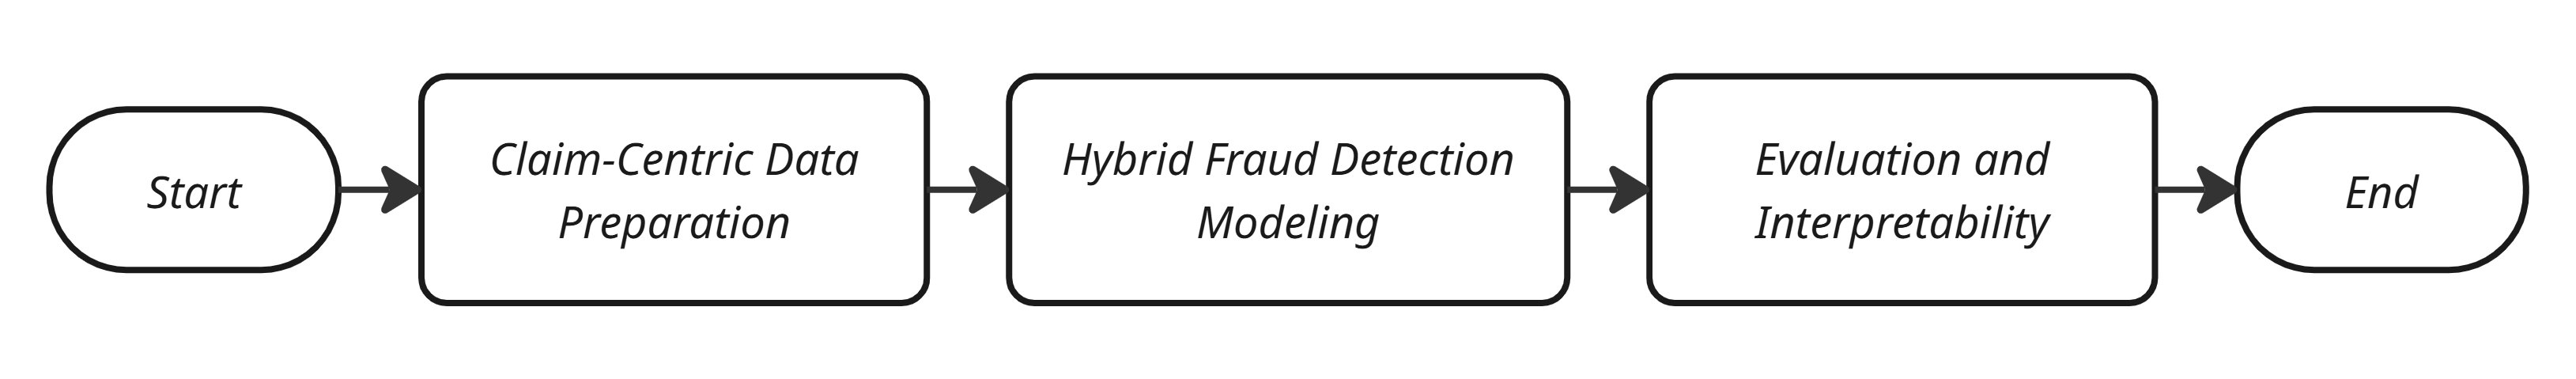
\includegraphics[width=5.51181in,height=0.81042in]{media/media/image6.png}

\phantomsection\label{_Toc228109334}{}Gambar 3. 1 Desain Sistem Deteksi Potensi Fraud Klaim

Berdasarkan Gambar 3.1, alur sistem dimulai dari tahap persiapan data berbasis klaim untuk membentuk dataset analitis yang terstruktur. Dataset tersebut selanjutnya digunakan pada tahap~\emph{hybrid fraud detection modeling}~untuk membangun model deteksi risiko berbasis pseudo-label dan~\emph{supervised learning}. Setelah model final diperoleh, proses dilanjutkan ke tahap evaluasi dan interpretabilitas guna menilai performa model serta menjelaskan faktor-faktor yang berkontribusi terhadap prediksi klaim berisiko tinggi. Untuk memberikan pembahasan yang lebih rinci, masing-masing komponen utama tersebut dijelaskan pada subbagian berikutnya.

\subsection{\texorpdfstring{\emph{Claim-Centric Data Preparation}}{Claim-Centric Data Preparation}}\label{claim-centric-data-preparation}

Tahap~\emph{Claim-Centric Data Preparation}~merupakan bagian awal dari sistem yang bertujuan mengubah data mentah BPJS menjadi dataset analisis berbasis klaim. Pada tahap ini, setiap klaim diposisikan sebagai unit analisis utama, sehingga seluruh proses integrasi, pembersihan, dan pembentukan fitur diarahkan untuk menghasilkan satu representasi data yang utuh pada level klaim. Pendekatan ini dipilih agar deteksi potensi fraud tidak hanya mengandalkan satu atribut biaya, tetapi juga mempertimbangkan konteks peserta, diagnosis, histori layanan, dan karakteristik klinis yang menyertai klaim tersebut.

Sumber data yang digunakan pada penelitian ini terdiri atas beberapa tabel utama, yaitu~FKRTL,~kepesertaan,~diagnosissekunder,~FKTP kapitasi, dan~nonkapitasi. Masing-masing tabel memiliki fungsi yang berbeda dalam \emph{pipeline} analisis, mulai dari penyediaan informasi inti klaim, data profil peserta, rincian diagnosis tambahan, hingga histori pemanfaatan layanan sebelum terjadinya klaim. Ringkasan fungsi setiap tabel dan perannya dalam pipeline ditunjukkan pada Tabel 3.2.

\phantomsection\label{_Toc228109621}{}Tabel 3. 2 Tabel Sumber Data yang Digunakan

\begin{longtable}[]{@{}
  >{\raggedright\arraybackslash}p{(\columnwidth - 4\tabcolsep) * \real{0.2510}}
  >{\raggedright\arraybackslash}p{(\columnwidth - 4\tabcolsep) * \real{0.3776}}
  >{\raggedright\arraybackslash}p{(\columnwidth - 4\tabcolsep) * \real{0.3714}}@{}}
\toprule\noalign{}
\begin{minipage}[b]{\linewidth}\raggedright
\textbf{Nama Tabel}
\end{minipage} & \begin{minipage}[b]{\linewidth}\raggedright
\textbf{Fungsi}
\end{minipage} & \begin{minipage}[b]{\linewidth}\raggedright
\textbf{Peran dalam \emph{Pipeline}}
\end{minipage} \\
\midrule\noalign{}
\endhead
\bottomrule\noalign{}
\endlastfoot
FKRTL & Menyediakan data klaim layanan lanjutan & \emph{Fact table} utama dan unit analisis \\
kepesertaan & Menyediakan atribut peserta & Pengayaan profil peserta \\
diagnosissekunder & Menyediakan diagnosis tambahan & Agregasi diagnosis sekunder per klaim \\
FKTP kapitasi & Menyediakan histori layanan tingkat pertama & Pembentukan fitur histori layanan \\
nonkapitasi & Menyediakan histori layanan nonkapitasi & Pembentukan fitur histori biaya dan utilisasi \\
\end{longtable}

Sebagaimana dirangkum pada Tabel 3.2, tabel~FKRTL~digunakan sebagai pusat analisis karena merepresentasikan klaim layanan lanjutan yang menjadi objek utama deteksi risiko. Tabel~kepesertaan~digunakan untuk memperkaya klaim dengan atribut peserta, sedangkan tabel~diagnosissekunder~digunakan untuk menangkap intensitas dan keragaman diagnosis tambahan pada tiap klaim. Sementara itu, tabel~FKTP kapitasi~dan~nonkapitasi~digunakan untuk membentuk histori layanan sebelum tanggal klaim, sehingga model dapat mempertimbangkan pola utilisasi layanan sebelumnya sebagai bagian dari konteks analisis.

Sebelum proses integrasi dilakukan, sistem terlebih dahulu menerapkan~\emph{knowledge-driven column mapping}~berdasarkan~\emph{data dictionary}~BPJS. Tahap ini bertujuan untuk menerjemahkan kode-kode kolom mentah menjadi nama variabel yang lebih eksplisit, konsisten, dan mudah diinterpretasikan. Dengan pendekatan ini, proses analisis tidak hanya bergantung pada nama kolom asli, tetapi juga pada makna domain yang melekat pada setiap variabel. Ringkasan variabel yang dipetakan dari~\emph{data dictionary}~dan digunakan dalam penelitian ini ditunjukkan pada Tabel 3.3.

\phantomsection\label{_Toc228109622}{}Tabel 3. 3 Ringkasan Pemetaan Variabel Berdasarkan Data Dictionary

\begin{longtable}[]{@{}
  >{\raggedright\arraybackslash}p{(\columnwidth - 8\tabcolsep) * \real{0.1999}}
  >{\raggedright\arraybackslash}p{(\columnwidth - 8\tabcolsep) * \real{0.1999}}
  >{\raggedright\arraybackslash}p{(\columnwidth - 8\tabcolsep) * \real{0.2001}}
  >{\raggedright\arraybackslash}p{(\columnwidth - 8\tabcolsep) * \real{0.1999}}
  >{\raggedright\arraybackslash}p{(\columnwidth - 8\tabcolsep) * \real{0.2001}}@{}}
\toprule\noalign{}
\begin{minipage}[b]{\linewidth}\raggedright
\textbf{Nama Tabel}
\end{minipage} & \begin{minipage}[b]{\linewidth}\raggedright
\textbf{Kode Kolom Asli}
\end{minipage} & \begin{minipage}[b]{\linewidth}\raggedright
\textbf{Nama Variabel Hasil Mapping}
\end{minipage} & \begin{minipage}[b]{\linewidth}\raggedright
\textbf{Deskripsi Singkat}
\end{minipage} & \begin{minipage}[b]{\linewidth}\raggedright
\textbf{Digunakan pada Tahap}
\end{minipage} \\
\midrule\noalign{}
\endhead
\bottomrule\noalign{}
\endlastfoot
kepesertaan & PSTV01 & id\_peserta & Identitas unik peserta BPJS & Integrasi data \\
kepesertaan & PSTV03 & tanggal\_lahir & Tanggal lahir peserta untuk menghitung usia & Feature engineering \\
kepesertaan & PSTV04 & hubungan\_keluarga & Status hubungan peserta dalam keluarga & Feature engineering \\
kepesertaan & PSTV05 & jenis\_kelamin & Jenis kelamin peserta & Feature engineering \\
kepesertaan & PSTV07 & kelas\_rawat\_hak & Hak kelas rawat peserta & Feature engineering \\
kepesertaan & PSTV08 & segmen\_kepesertaan & Kategori kepesertaan peserta & Feature engineering \\
kepesertaan & PSTV11 & kepemilikan\_fktp & Status kepemilikan FKTP terdaftar & Feature engineering \\
kepesertaan & PSTV12 & jenis\_fktp & Jenis FKTP peserta & Feature engineering \\
kepesertaan & PSTV17 & status\_kepesertaan & Status aktif atau nonaktif kepesertaan & Feature engineering \\
fkrtl & FKL02 & id\_klaim & Identitas unik klaim kunjungan & Integrasi data \\
fkrtl & PSTV01 & id\_peserta & Identitas peserta pada data klaim & Integrasi data \\
fkrtl & FKP02 & id\_kunjungan\_fktp\_rujukan & Identitas rujukan FKTP ke FKRTL & Feature engineering \\
fkrtl & FKL03 & tanggal\_masuk & Tanggal masuk pelayanan rumah sakit & Integrasi data dan feature engineering \\
fkrtl & FKL04 & tanggal\_pulang & Tanggal keluar pelayanan rumah sakit & Feature engineering \\
fkrtl & FKL07 & kepemilikan\_faskes & Status kepemilikan fasilitas kesehatan & Feature engineering \\
fkrtl & FKL08 & jenis\_faskes & Jenis fasilitas kesehatan & Feature engineering \\
fkrtl & FKL09 & tipe\_faskes & Tipe atau kelas fasilitas kesehatan & Feature engineering \\
fkrtl & FKL10 & tingkat\_layanan & Tingkat layanan, seperti rawat inap atau rawat jalan & Feature engineering \\
fkrtl & FKL11 & poli\_tujuan & Poliklinik tujuan pelayanan & Feature engineering \\
fkrtl & FKL12 & segmen\_peserta\_klaim & Kategori kepesertaan saat klaim terjadi & Feature engineering \\
fkrtl & FKL13 & kelas\_rawat\_klaim & Kelas rawat yang ditagihkan pada klaim & Feature engineering \\
fkrtl & FKL14 & status\_pulang & Status akhir pasien setelah pelayanan & Feature engineering \\
fkrtl & FKL15A & grup\_diagnosis\_utama & Kelompok diagnosis utama pada level makro & Feature engineering \\
fkrtl & FKL16 & kode\_diagnosis\_utama\_icd10 & Kode diagnosis utama ICD-10 & Feature engineering \\
fkrtl & FKL17A & grup\_tindakan\_utama & Kelompok tindakan utama & Feature engineering \\
fkrtl & FKL18 & kode\_tindakan\_utama\_icd9cm & Kode tindakan utama ICD-9-CM & Feature engineering \\
fkrtl & FKL20 & jenis\_inacbg & Kategori klaim INA-CBG & Feature engineering \\
fkrtl & FKL21 & kategori\_tindakan & Kategori tindakan medis & Feature engineering \\
fkrtl & FKL22 & severity\_level & Tingkat keparahan klaim & Feature engineering dan modeling \\
fkrtl & FKL23 & jenis\_pelayanan & Jenis pelayanan yang diberikan & Feature engineering \\
fkrtl & FKL30 / FKL31* & regional\_tarif & Zona atau regional tarif BPJS & Feature engineering \\
fkrtl & FKL31 / FKL32* & tarif\_inacbg\_dasar & Tarif dasar paket INA-CBG & Feature engineering \\
fkrtl & FKL34 & biaya\_special\_cmg\_1 & Biaya top-up atau special CMG komponen 1 & Feature engineering \\
fkrtl & FKL37 & biaya\_special\_cmg\_2 & Biaya top-up atau special CMG komponen 2 & Feature engineering \\
fkrtl & FKL40 & biaya\_special\_cmg\_3 & Biaya top-up atau special CMG komponen 3 & Feature engineering \\
fkrtl & FKL43 & biaya\_special\_cmg\_4 & Biaya top-up atau special CMG komponen 4 & Feature engineering \\
fkrtl & FKL46 & biaya\_special\_cmg\_5 & Biaya top-up atau special CMG komponen 5 & Feature engineering \\
fkrtl & FKL47 / FKL48* & tarif\_grouping / tarif\_disetujui & Nilai biaya grouping dan biaya klaim yang disetujui & Feature engineering dan modeling \\
diagnosissekunder & FKL02 & id\_klaim & Identitas klaim untuk relasi dengan FKRTL & Integrasi data \\
diagnosissekunder & FKL24 & kode\_diagnosis\_sekunder & Kode diagnosis sekunder ICD-10 & Agregasi diagnosis \\
diagnosissekunder & FKL24A & grup\_diagnosis\_sekunder & Kelompok diagnosis sekunder & Agregasi diagnosis \\
fktpkapitasi & PSTV01 & id\_peserta & Identitas peserta pada layanan FKTP kapitasi & Pembentukan histori layanan \\
fktpkapitasi & FKP04** & tanggal\_pelayanan\_fktp & Tanggal pelayanan FKTP & Pembentukan histori layanan \\
nonkapitasi & PSTV01 & id\_peserta & Identitas peserta pada layanan nonkapitasi & Pembentukan histori layanan \\
nonkapitasi & PNK04 / PNK03** & tanggal\_pelayanan\_nonkap & Tanggal pelayanan nonkapitasi & Pembentukan histori layanan \\
nonkapitasi & PNK18 & tarif\_disetujui\_nonkap & Biaya nonkapitasi yang disetujui & Pembentukan histori biaya layanan \\
\end{longtable}

\emph{* Penomoran kode pada data dictionary dan notebook menunjukkan sedikit perbedaan versi pada beberapa variabel tarif, namun nama variabel hasil mapping pada penelitian ini mengikuti implementasi final pada notebook.}

\emph{** Penamaan tanggal layanan mengikuti implementasi variabel pada notebook final untuk kebutuhan pembentukan histori layanan.}

Tabel 3.3 menunjukkan bahwa tidak seluruh kolom pada~\emph{data dictionary}~digunakan dalam penelitian ini. Hanya variabel yang relevan terhadap integrasi data, pembentukan fitur, dan pemodelan yang dipertahankan. Pemilihan ini dilakukan agar pipeline tetap fokus pada variabel yang memiliki kontribusi langsung terhadap pembentukan dataset analisis dan deteksi potensi fraud. Dengan demikian, tabel pemetaan pada Bab 3 berfungsi sebagai ringkasan variabel terpilih, sedangkan detail lengkap~\emph{data dictionary}~dapat ditempatkan pada lampiran.

Setelah proses pemetaan kolom dilakukan, sistem menetapkan~FKRTL~sebagai~\emph{fact table}~utama. Pemilihan ini didasarkan pada pertimbangan bahwa~FKRTL~merepresentasikan entitas klaim yang paling sesuai dengan tujuan penelitian, yaitu mendeteksi potensi fraud atau upcoding pada level klaim. Dengan menjadikan~FKRTL~sebagai pusat analisis, setiap baris data pada dataset akhir mewakili satu klaim, sehingga proses deteksi risiko dapat dilakukan secara lebih spesifik dan sesuai dengan kebutuhan analisis transaksi klaim.

Integrasi data kemudian dilakukan dengan menambahkan atribut dari tabel lain ke dalam struktur klaim utama. Tabel~kepesertaan~digunakan untuk menambahkan atribut seperti jenis kelamin, tanggal lahir, dan status kepesertaan. Tabel~diagnosissekunder~digunakan untuk membentuk agregasi diagnosis sekunder per~id\_klaim, misalnya jumlah diagnosis sekunder dan jumlah kelompok diagnosis sekunder. Selain itu, tabel~FKTP kapitasi~dan~nonkapitasi~digunakan untuk membangun fitur histori layanan sebelum tanggal klaim, sehingga sistem dapat menangkap intensitas dan pola pemanfaatan layanan yang mendahului klaim. Alur lengkap proses ini ditunjukkan pada Gambar 3.2.

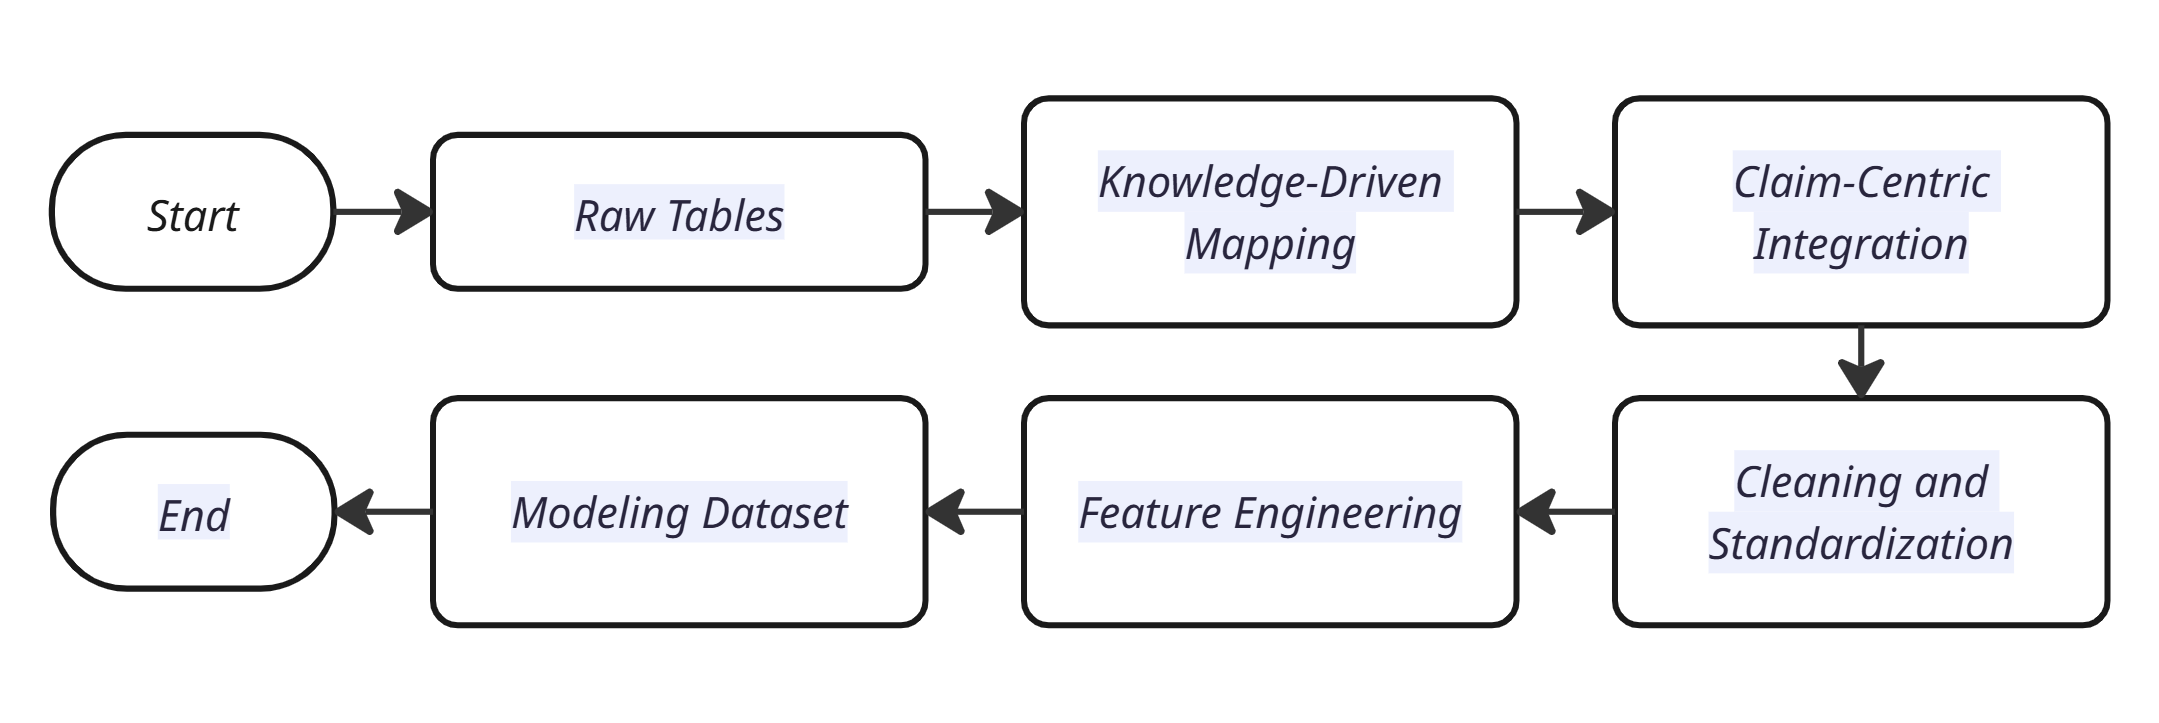
\includegraphics[width=5.51181in,height=1.84583in]{media/media/image7.png}

\phantomsection\label{_Toc228109335}{}Gambar 3. 2 Alur Claim-Centric Data Preparation

Berdasarkan Gambar 3.2, tahap~\emph{Claim-Centric Data Preparation}~dimulai dari pemuatan tabel mentah, dilanjutkan dengan~\emph{knowledge-driven mapping}, integrasi berbasis klaim, pembersihan dan standardisasi data, rekayasa fitur, hingga pembentukan dataset pemodelan. Urutan ini menunjukkan bahwa penyusunan dataset tidak dilakukan secara langsung, melainkan melalui tahapan yang saling bergantung agar data yang dihasilkan bersifat konsisten, informatif, dan siap digunakan pada tahap pemodelan.

Setelah integrasi data selesai, sistem melakukan proses~\emph{cleaning}~dan~\emph{standardization}~untuk memastikan bahwa seluruh variabel berada pada format yang sesuai. Tahap ini mencakup standardisasi identifier, konversi tipe data tanggal, konversi nilai numerik untuk atribut biaya dan tingkat keparahan, serta penanganan nilai kosong dan nilai tidak valid. Proses ini penting karena data yang berasal dari beberapa tabel berbeda berpotensi memiliki format yang tidak seragam. Tanpa standardisasi, kualitas dataset akhir dapat menurun dan memengaruhi performa model pada tahap berikutnya.

Tahap berikutnya adalah~\emph{feature engineering}, yaitu pembentukan variabel turunan yang dirancang untuk menangkap sinyal risiko fraud secara lebih jelas. Fitur yang dibentuk pada penelitian ini dikelompokkan ke dalam beberapa kategori, yaitu fitur demografis, biaya, klinis, diagnosis, histori layanan, dan rasio turunan. Setiap kelompok fitur memiliki tujuan analitis yang berbeda, misalnya untuk menangkap profil peserta, beban biaya klaim, kompleksitas kondisi klinis, maupun pola historis pemanfaatan layanan. Ringkasan kelompok fitur yang digunakan ditunjukkan pada Tabel 3.4.

\phantomsection\label{_Toc228109623}{}Tabel 3. 4 Kelompok Fitur Hasil Rekayasa Fitur

\begin{longtable}[]{@{}
  >{\raggedright\arraybackslash}p{(\columnwidth - 4\tabcolsep) * \real{0.1783}}
  >{\raggedright\arraybackslash}p{(\columnwidth - 4\tabcolsep) * \real{0.5316}}
  >{\raggedright\arraybackslash}p{(\columnwidth - 4\tabcolsep) * \real{0.2901}}@{}}
\toprule\noalign{}
\begin{minipage}[b]{\linewidth}\raggedright
\textbf{Kelompok Fitur}
\end{minipage} & \begin{minipage}[b]{\linewidth}\raggedright
\textbf{Contoh Variabel}
\end{minipage} & \begin{minipage}[b]{\linewidth}\raggedright
\textbf{Tujuan Analitis}
\end{minipage} \\
\midrule\noalign{}
\endhead
\bottomrule\noalign{}
\endlastfoot
Demografis & usia, gender\_singkat & Menggambarkan profil dasar peserta \\
Biaya & tarif\_disetujui, tarif\_inacbg\_dasar, biaya\_per\_hari & Menangkap pola beban biaya klaim \\
Klinis & severity\_level, lama\_rawat\_hari, total\_special\_cmg & Menunjukkan tingkat keparahan dan kompleksitas klinis \\
Diagnosis & jumlah\_diagnosis\_sekunder, jumlah\_grup\_diagnosis\_sekunder & Mengukur intensitas diagnosis tambahan \\
Histori layanan & fktp\_hist\_count\_before, nonkap\_hist\_count\_before & Menangkap pola utilisasi layanan sebelum klaim \\
Rasio turunan & rasio\_tarif\_setuju\_vs\_dasar, rasio\_biaya\_klaim\_vs\_histori\_nonkap & Menyoroti ketidakwajaran relatif antar komponen biaya \\
\end{longtable}

Sebagaimana ditunjukkan pada Tabel 3.4, fitur-fitur hasil rekayasa tidak dibangun secara acak, melainkan disusun berdasarkan hubungan antara informasi administratif, klinis, finansial, dan historis yang terdapat dalam data klaim. Dengan pendekatan ini, dataset akhir tidak hanya memuat variabel mentah, tetapi juga representasi yang lebih kaya untuk menangkap pola potensi fraud atau upcoding.

Keluaran akhir dari tahap ini adalah terbentuknya~model\_df, yaitu dataset pemodelan yang berisi identitas klaim dan variabel-variabel hasil integrasi serta rekayasa fitur yang telah siap dipakai pada tahap pemodelan. Dataset ini menjadi fondasi bagi tahap berikutnya, yaitu~\emph{Hybrid Fraud Detection Modeling}, di mana pseudo-label dibentuk dan model~\emph{supervised learning}~dibandingkan untuk memperoleh konfigurasi deteksi yang paling sesuai.

\subsection{\texorpdfstring{\emph{Hybrid Fraud Detection Modeling}}{Hybrid Fraud Detection Modeling}}\label{hybrid-fraud-detection-modeling}

Tahap~\emph{Hybrid Fraud Detection Modeling}~merupakan inti dari proses analisis pada penelitian ini, karena pada bagian inilah dataset berbasis klaim yang telah dibentuk pada tahap sebelumnya diubah menjadi sistem deteksi risiko yang dapat menghasilkan prediksi. Pendekatan yang digunakan bersifat~\emph{hybrid}, yaitu menggabungkan~\emph{unsupervised learning}~untuk membentuk pseudo-label awal dan~\emph{supervised learning}~untuk membangun model klasifikasi final. Pemilihan pendekatan ini dilakukan untuk menjawab keterbatasan utama pada data klaim, yaitu tidak tersedianya label fraud transaksi riil pada level klaim yang dapat langsung digunakan sebagai target pembelajaran.

Tahap awal dalam komponen ini adalah pemilihan fitur untuk~\emph{unsupervised stage}. Fitur yang digunakan pada tahap ini dipilih dari variabel-variabel numerik yang merepresentasikan karakteristik biaya, klinis, diagnosis, dan histori layanan yang paling relevan untuk mendeteksi anomali pola klaim. Pemilihan fitur pada tahap~\emph{unsupervised}~berbeda dari tahap~\emph{supervised}, karena tujuan utamanya bukan untuk langsung mengklasifikasikan klaim, melainkan untuk membangun dasar penandaan awal terhadap klaim yang memiliki karakteristik menyimpang dari Meioritas populasi.

Pseudo-label kemudian dibentuk menggunakan algoritma~\emph{Isolation Forest}. Algoritma ini digunakan untuk mendeteksi klaim yang memiliki pola anomali berdasarkan kombinasi fitur yang telah dipilih pada tahap sebelumnya. Dalam konteks penelitian ini, klaim yang teridentifikasi sebagai anomali diperlakukan sebagai klaim berisiko dan digunakan sebagai dasar pembentukan pseudo-label. Dengan demikian, sistem dapat menghasilkan target pembelajaran awal tanpa bergantung pada label fraud final yang tidak tersedia secara langsung pada data transaksi klaim.

Setelah proses~\emph{pseudo-labeling}~dilakukan, dataset dibagi menjadi tiga subset utama, yaitu~\emph{train},~\emph{validation}, dan~\emph{test}. Pembagian ini dilakukan untuk menjaga pemisahan fungsi setiap subset, yaitu pelatihan model, pemilihan konfigurasi terbaik, dan evaluasi akhir. Pada tahap ini juga dilakukan~\emph{preprocessing}~agar data siap digunakan oleh model, termasuk penanganan nilai kosong, transformasi variabel numerik, dan pengkodean variabel kategorikal. Alur utama proses pemodelan hybrid dari pseudo-labeling hingga pemilihan model final ditunjukkan pada Gambar 3.3.

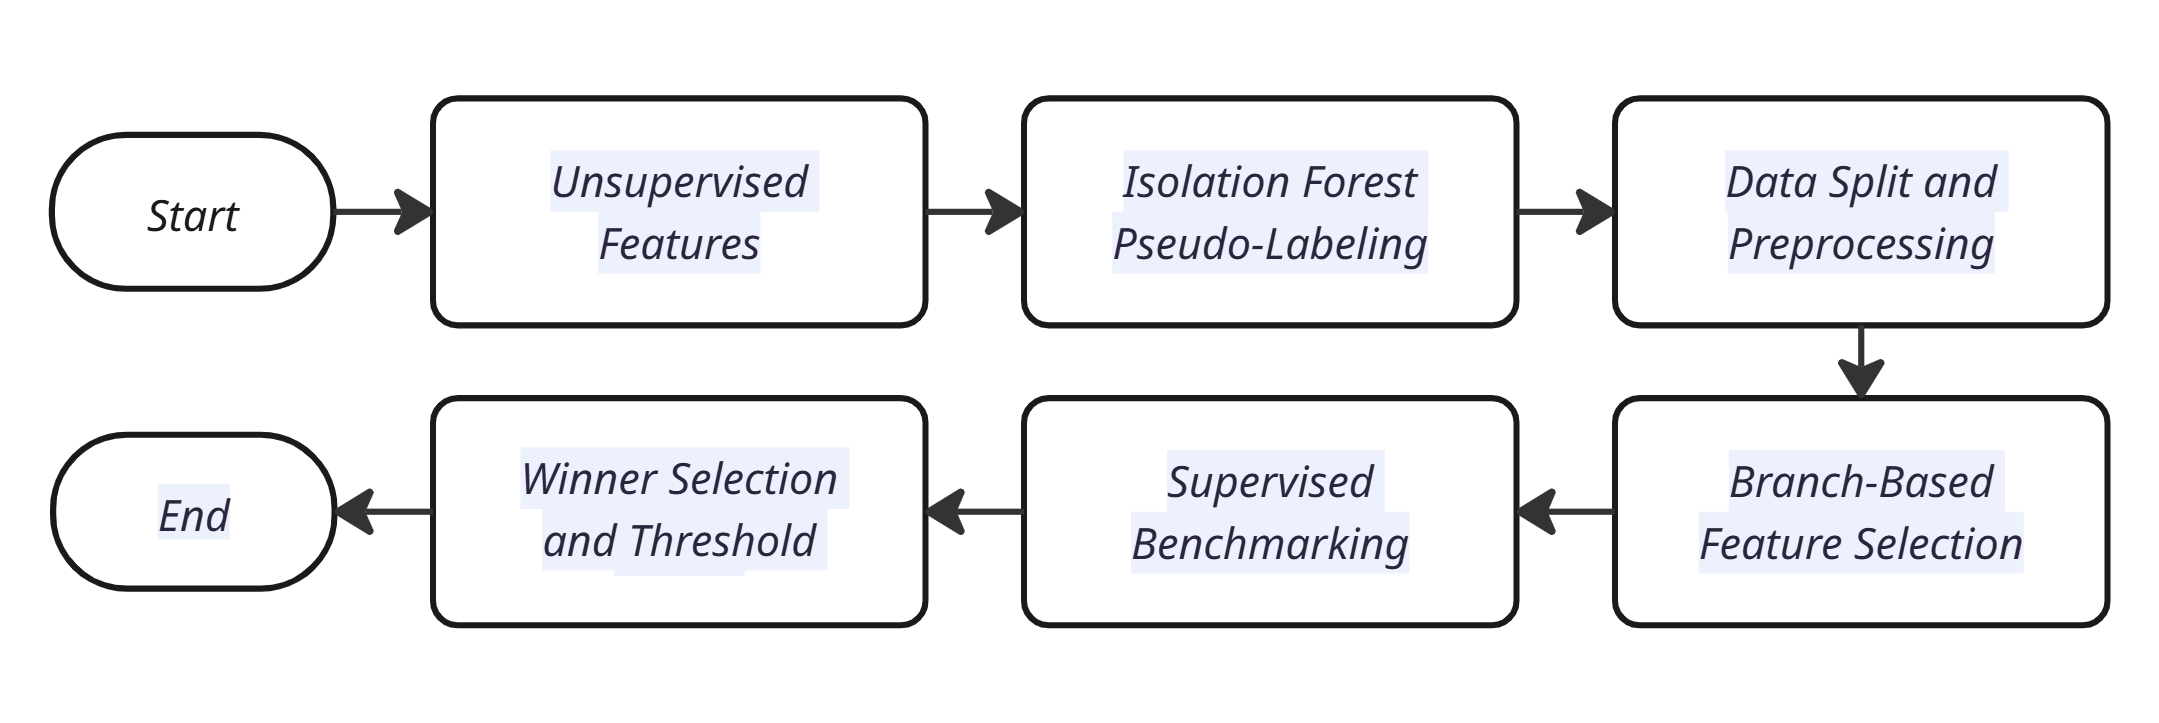
\includegraphics[width=5.51181in,height=1.84583in]{media/media/image8.png}

\phantomsection\label{_Toc228109336}{}Gambar 3. 3 Alur Hybrid Fraud Detection Modeling

Berdasarkan Gambar 3.3, alur pemodelan dimulai dari pemilihan fitur untuk tahap~\emph{unsupervised}, dilanjutkan dengan pembentukan pseudo-label menggunakan~\emph{Isolation Forest}, pembagian data dan~\emph{preprocessing}, seleksi fitur berbasis beberapa cabang,~\emph{benchmarking}~model~\emph{supervised}, hingga pemilihan model terbaik dan penentuan~\emph{threshold}~klasifikasi. Urutan ini menunjukkan bahwa model final pada penelitian ini tidak diperoleh secara langsung dari satu algoritma, melainkan melalui serangkaian tahapan seleksi dan evaluasi yang dirancang untuk menghasilkan konfigurasi deteksi risiko yang paling sesuai.

Setelah~\emph{preprocessing}~dilakukan, sistem menerapkan~\emph{branch-based feature selection}~untuk membandingkan beberapa strategi pemilihan fitur. Pendekatan ini digunakan agar sistem tidak bergantung pada satu skema fitur tunggal, melainkan mengevaluasi beberapa cabang seleksi fitur yang memiliki dasar pertimbangan berbeda. Dengan cara ini, penelitian dapat menilai apakah model memberikan performa terbaik pada fitur yang dipilih secara berbasis pengetahuan domain, berbasis korelasi statistik, berbasis~\emph{variance inflation factor}, berbasis~\emph{permutation importance}, atau pada kombinasi dari beberapa strategi tersebut. Ringkasan branch seleksi fitur yang digunakan ditunjukkan pada Tabel 3.5.

\phantomsection\label{_Toc228109624}{}Tabel 3. 5 Branch Feature Selection yang Digunakan

\begin{longtable}[]{@{}
  >{\raggedright\arraybackslash}p{(\columnwidth - 4\tabcolsep) * \real{0.1862}}
  >{\raggedright\arraybackslash}p{(\columnwidth - 4\tabcolsep) * \real{0.3892}}
  >{\raggedright\arraybackslash}p{(\columnwidth - 4\tabcolsep) * \real{0.4246}}@{}}
\toprule\noalign{}
\begin{minipage}[b]{\linewidth}\raggedright
\textbf{Branch}
\end{minipage} & \begin{minipage}[b]{\linewidth}\raggedright
\textbf{Prinsip Seleksi}
\end{minipage} & \begin{minipage}[b]{\linewidth}\raggedright
\textbf{Tujuan}
\end{minipage} \\
\midrule\noalign{}
\endhead
\bottomrule\noalign{}
\endlastfoot
Domain Expert & Memilih fitur berdasarkan relevansi domain klaim kesehatan & Memastikan fitur penting secara substantif tetap dipertahankan \\
Correlation & Menghapus fitur yang sangat berkorelasi & Mengurangi redundansi antar fitur \\
VIF & Menyeleksi fitur berdasarkan multikolinearitas & Menjaga stabilitas model dan mengurangi ketergantungan antar variabel \\
Permutation & Memilih fitur berdasarkan kontribusi prediktif terhadap model & Mengidentifikasi fitur yang paling berpengaruh terhadap performa \\
Combined & Menggabungkan hasil seleksi dari beberapa strategi & Membentuk himpunan fitur yang lebih seimbang \\
\end{longtable}

Sebagaimana dirangkum pada Tabel 3.5, setiap~\emph{branch}~memiliki prinsip seleksi dan tujuan yang berbeda.~\emph{Branch}~berbasis~\emph{domain expert}~mempertahankan fitur yang dianggap penting secara substantif dalam konteks klaim kesehatan, sedangkan~\emph{branch}~berbasis korelasi dan~\emph{VIF}~berfokus pada pengurangan redundansi antar fitur. Sementara itu,~\emph{branch}~berbasis~\emph{permutation importance}~menekankan kontribusi prediktif fitur terhadap model, dan~\emph{branch combined}~digunakan untuk memperoleh himpunan fitur yang lebih seimbang antara relevansi domain dan stabilitas statistik.

Tahap berikutnya adalah~\emph{supervised benchmarking}, yaitu membandingkan beberapa model klasifikasi untuk mengetahui model mana yang memberikan performa terbaik terhadap pseudo-label yang telah dibentuk. Strategi ini digunakan agar pemilihan model final bersifat empiris dan tidak didasarkan pada asumsi awal terhadap satu algoritma tertentu. Model-model yang dibandingkan pada penelitian ini mencakup model linear, model ensemble berbasis pohon, serta model~\emph{boosting}~yang umum digunakan pada permasalahan klasifikasi tabular. Daftar model yang digunakan dalam proses pembandingan disajikan pada Tabel 3.6.

\phantomsection\label{_Toc228109625}{}Tabel 3. 6 Daftar Model Supervised yang Dibandingkan

\begin{longtable}[]{@{}
  >{\raggedright\arraybackslash}p{(\columnwidth - 4\tabcolsep) * \real{0.1963}}
  >{\raggedright\arraybackslash}p{(\columnwidth - 4\tabcolsep) * \real{0.2972}}
  >{\raggedright\arraybackslash}p{(\columnwidth - 4\tabcolsep) * \real{0.5065}}@{}}
\toprule\noalign{}
\begin{minipage}[b]{\linewidth}\raggedright
\textbf{Model}
\end{minipage} & \begin{minipage}[b]{\linewidth}\raggedright
\textbf{Jenis}
\end{minipage} & \begin{minipage}[b]{\linewidth}\raggedright
\textbf{Fungsi dalam Benchmarking}
\end{minipage} \\
\midrule\noalign{}
\endhead
\bottomrule\noalign{}
\endlastfoot
Logistic Regression & Model linear & Menjadi baseline untuk melihat performa klasifikasi sederhana \\
Random Forest & Ensemble bagging berbasis pohon & Menangkap hubungan nonlinier dan memberikan pembanding model ensemble \\
Linear SVM & Model margin linear & Menjadi pembanding pemisahan kelas pada ruang fitur hasil preprocessing \\
XGBoost & Gradient boosting berbasis pohon & Menguji performa boosting dengan optimasi prediktif tinggi \\
LightGBM & Gradient boosting berbasis histogram & Menjadi pembanding boosting yang efisien pada data tabular \\
CatBoost & Gradient boosting berbasis pohon kategorikal & Menguji kemampuan boosting pada data dengan kombinasi fitur numerik dan kategorikal \\
\end{longtable}

Tabel 3.6 menunjukkan bahwa proses~\emph{benchmarking}~dilakukan secara komparatif terhadap beberapa keluarga model yang memiliki karakteristik berbeda.~\emph{Logistic Regression}~digunakan sebagai model dasar untuk melihat performa pada pola hubungan yang lebih sederhana, sedangkan~\emph{Random Forest},~\emph{XGBoost},~\emph{LightGBM}, dan~\emph{CatBoost}~digunakan untuk menangkap hubungan nonlinier yang lebih kompleks. Selain itu,~\emph{Linear SVM}~digunakan sebagai pembanding tambahan untuk melihat kemampuan pemisahan kelas pada ruang fitur yang telah diproses. Dengan susunan model seperti ini, sistem memiliki dasar evaluasi yang lebih kuat dalam memilih model terbaik.

Hasil dari tahap~\emph{benchmarking}~kemudian digunakan dalam proses~\emph{winner selection}. Pada tahap ini, sistem memilih kombinasi terbaik antara~\emph{branch}~fitur dan model klasifikasi berdasarkan performa evaluasi pada data~\emph{validation}. Setelah model pemenang diperoleh, dilakukan~\emph{threshold tuning}~untuk menentukan ambang klasifikasi yang paling sesuai dengan tujuan deteksi potensi fraud. Proses ini penting karena keputusan akhir model tidak hanya ditentukan oleh probabilitas prediksi, tetapi juga oleh ambang yang digunakan untuk memisahkan klaim berisiko dan klaim normal.

Untuk memudahkan pemahaman hubungan antar tahap pada komponen ini, ringkasan alur pemodelan hybrid dapat disajikan pada Tabel 3.7. Tabel tersebut merangkum input, proses, dan output pada setiap tahap utama, sehingga pembaca dapat melihat keterkaitan antara pembentukan pseudo-label, seleksi fitur, pembandingan model, hingga pemilihan model final secara lebih cepat dan sistematis.

\phantomsection\label{_Toc228109626}{}Tabel 3. 7 Ringkasan Tahap Pemodelan Hybrid

\begin{longtable}[]{@{}
  >{\raggedright\arraybackslash}p{(\columnwidth - 6\tabcolsep) * \real{0.2368}}
  >{\raggedright\arraybackslash}p{(\columnwidth - 6\tabcolsep) * \real{0.2240}}
  >{\raggedright\arraybackslash}p{(\columnwidth - 6\tabcolsep) * \real{0.3020}}
  >{\raggedright\arraybackslash}p{(\columnwidth - 6\tabcolsep) * \real{0.2372}}@{}}
\toprule\noalign{}
\begin{minipage}[b]{\linewidth}\raggedright
\textbf{Tahap}
\end{minipage} & \begin{minipage}[b]{\linewidth}\raggedright
\textbf{Input}
\end{minipage} & \begin{minipage}[b]{\linewidth}\raggedright
\textbf{Proses}
\end{minipage} & \begin{minipage}[b]{\linewidth}\raggedright
\textbf{Output}
\end{minipage} \\
\midrule\noalign{}
\endhead
\bottomrule\noalign{}
\endlastfoot
Pemilihan fitur unsupervised & Dataset hasil data preparation & Menentukan fitur numerik yang relevan untuk deteksi anomali & Set fitur unsupervised \\
Pseudo-labeling & Fitur unsupervised & Mendeteksi anomali menggunakan Isolation Forest & Anomaly score dan pseudo-label \\
Data split dan preprocessing & Dataset dengan pseudo-label & Membagi data dan menyiapkan fitur numerik serta kategorikal & Train, validation, test yang siap model \\
Branch-based feature selection & Data train hasil preprocessing & Menyeleksi fitur melalui beberapa branch & Beberapa kandidat set fitur \\
Supervised benchmarking & Data train dan validation & Membandingkan performa beberapa model klasifikasi & Hasil benchmarking model \\
Winner selection dan threshold tuning & Hasil benchmarking & Memilih model terbaik dan menentukan threshold klasifikasi & Model final dan threshold terbaik \\
\end{longtable}

Berdasarkan Tabel 3.7, dapat dilihat bahwa komponen~\emph{Hybrid Fraud Detection Modeling}~tidak hanya berfungsi sebagai tahap pelatihan model, tetapi juga sebagai kerangka seleksi bertingkat yang memastikan model final diperoleh melalui proses yang terkontrol. Tahap ini menghasilkan model terbaik beserta konfigurasi ambang klasifikasi yang selanjutnya digunakan pada komponen evaluasi dan interpretabilitas hasil.

\subsection{\texorpdfstring{\emph{Evaluation and Interpretability}}{Evaluation and Interpretability}}\label{evaluation-and-interpretability}

Tahap~\emph{Evaluation and Interpretability}~merupakan komponen akhir dalam perancangan sistem yang bertujuan menilai performa model final sekaligus menjelaskan alasan di balik prediksi yang dihasilkan. Pada penelitian ini, evaluasi tidak hanya diarahkan untuk mengetahui seberapa baik model membedakan klaim berisiko dan klaim normal, tetapi juga untuk memastikan bahwa hasil prediksi dapat ditafsirkan secara analitis. Pendekatan ini penting karena sistem deteksi fraud pada data klaim kesehatan harus mampu memberikan dasar penjelasan yang kuat, sehingga hasil yang diperoleh tidak berhenti pada skor risiko semata, melainkan dapat digunakan sebagai bahan pendukung untuk proses pemeriksaan lebih lanjut.

Setelah model pemenang dan~\emph{threshold}~klasifikasi diperoleh pada tahap sebelumnya, sistem melakukan~\emph{final model evaluation}~pada data~\emph{test}~yang tidak terlibat dalam proses pemilihan model. Evaluasi ini digunakan untuk menggambarkan kemampuan generalisasi model terhadap data yang belum pernah dilihat sebelumnya. Dengan demikian, performa yang diperoleh pada tahap ini merepresentasikan kualitas model final secara lebih objektif dibandingkan hasil evaluasi pada data pelatihan atau validasi.

Evaluasi model pada penelitian ini menggunakan beberapa metrik utama, yaitu~\emph{F1-score},~\emph{PR-AUC},~\emph{ROC-AUC},~\emph{precision},~\emph{recall}, dan~\emph{Matthews Correlation Coefficient}~(MCC). Pemilihan metrik tersebut didasarkan pada karakteristik permasalahan deteksi fraud, di mana distribusi kelas tidak seimbang dan kesalahan prediksi memiliki implikasi yang berbeda. Ringkasan metrik yang digunakan beserta fungsi dan alasan penggunaannya disajikan pada Tabel 3.8.

\phantomsection\label{_Toc228109627}{}Tabel 3. 8 Metrik Evaluasi Model

\begin{longtable}[]{@{}
  >{\raggedright\arraybackslash}p{(\columnwidth - 4\tabcolsep) * \real{0.1443}}
  >{\raggedright\arraybackslash}p{(\columnwidth - 4\tabcolsep) * \real{0.3429}}
  >{\raggedright\arraybackslash}p{(\columnwidth - 4\tabcolsep) * \real{0.5128}}@{}}
\toprule\noalign{}
\begin{minipage}[b]{\linewidth}\raggedright
\textbf{Metrik}
\end{minipage} & \begin{minipage}[b]{\linewidth}\raggedright
\textbf{Fungsi}
\end{minipage} & \begin{minipage}[b]{\linewidth}\raggedright
\textbf{Alasan Digunakan}
\end{minipage} \\
\midrule\noalign{}
\endhead
\bottomrule\noalign{}
\endlastfoot
F1-score & Mengukur keseimbangan antara precision dan recall & Cocok untuk deteksi fraud yang menuntut keseimbangan antara penangkapan kasus berisiko dan pengendalian kesalahan prediksi \\
PR-AUC & Mengukur kualitas pemeringkatan prediksi pada kelas positif & Relevan untuk data yang tidak seimbang karena lebih fokus pada kemampuan model mengenali klaim berisiko \\
ROC-AUC & Mengukur kemampuan model membedakan dua kelas secara umum & Memberikan gambaran umum separabilitas model \\
Precision & Mengukur proporsi klaim yang diprediksi berisiko dan benar-benar berisiko & Penting untuk menghindari terlalu banyak klaim normal yang salah ditandai \\
Recall & Mengukur proporsi klaim berisiko yang berhasil ditangkap model & Penting agar klaim berisiko tidak banyak terlewat \\
MCC & Mengukur kualitas klasifikasi secara seimbang & Cocok untuk kondisi kelas tidak seimbang karena mempertimbangkan seluruh komponen confusion matrix \\
\end{longtable}

Sebagaimana ditunjukkan pada Tabel 3.8, metrik evaluasi yang digunakan tidak hanya berfokus pada satu aspek performa.~\emph{Precision}~diperlukan untuk melihat ketepatan model dalam menandai klaim berisiko, sedangkan~\emph{recall}~diperlukan untuk menilai kemampuan model dalam menangkap klaim yang seharusnya tidak terlewat.~\emph{F1-score}~digunakan sebagai ukuran keseimbangan antara keduanya. Selain itu,~\emph{PR-AUC}~dan~\emph{ROC-AUC}~digunakan untuk menilai kualitas pemeringkatan skor prediksi, sedangkan~\emph{MCC}~digunakan karena mampu memberikan gambaran performa klasifikasi yang lebih seimbang pada kondisi distribusi kelas yang tidak merata.

Selain evaluasi performa, sistem ini juga dirancang untuk memberikan interpretasi terhadap hasil prediksi model. Interpretabilitas dilakukan pada dua tingkatan, yaitu interpretasi global dan interpretasi lokal. Interpretasi global digunakan untuk memahami fitur-fitur yang secara umum paling berpengaruh terhadap keputusan model, sedangkan interpretasi lokal digunakan untuk menjelaskan prediksi pada klaim tertentu yang memiliki tingkat risiko tinggi. Alur umum tahap evaluasi dan interpretabilitas pada penelitian ini ditunjukkan pada Gambar 3.4.

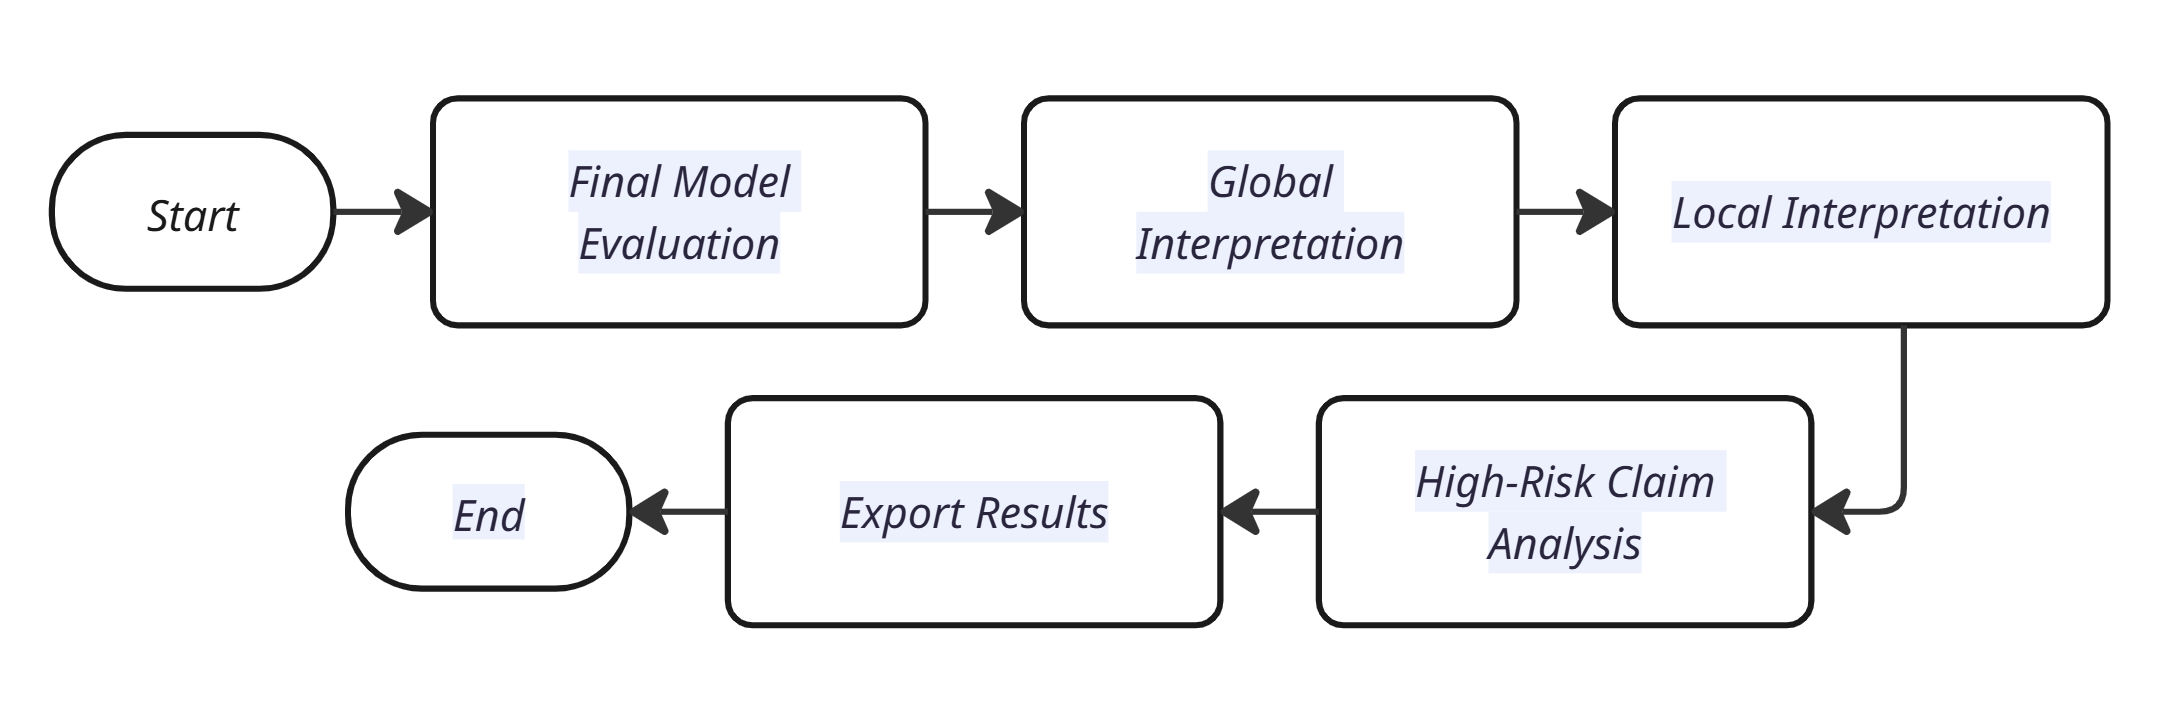
\includegraphics[width=5.51181in,height=1.84583in]{media/media/image9.png}

\phantomsection\label{_Toc228109337}{}Gambar 3. 4 Alur Evaluation and Interpretability

Berdasarkan Gambar 3.4, tahap ini dimulai dari evaluasi model final, kemudian dilanjutkan dengan interpretasi global, interpretasi lokal, analisis klaim berisiko tinggi, dan ekspor artefak hasil. Susunan ini menunjukkan bahwa keluaran sistem tidak hanya berupa angka performa, tetapi juga mencakup penjelasan fitur-fitur yang memengaruhi prediksi dan daftar klaim yang layak diprioritaskan untuk analisis lanjutan.

Interpretasi global pada penelitian ini dilakukan melalui~\emph{feature importance}~dan~\emph{SHAP}.~\emph{Feature importance}~digunakan untuk memberikan gambaran umum mengenai variabel mana yang paling dominan dalam proses pengambilan keputusan model. Sementara itu,~\emph{SHAP}~digunakan untuk menjelaskan arah dan besar kontribusi setiap fitur terhadap prediksi model secara lebih rinci. Dengan memadukan kedua teknik ini, penelitian tidak hanya memperoleh daftar fitur yang penting, tetapi juga dapat memahami bagaimana perubahan nilai suatu fitur berasosiasi dengan peningkatan atau penurunan risiko klaim.

Selain interpretasi global, penelitian ini juga menggunakan~\emph{Partial Dependence Plot}~(PDP) untuk melihat pola hubungan antara perubahan nilai fitur tertentu terhadap probabilitas fraud yang diprediksi model. Teknik ini membantu memperjelas bagaimana suatu fitur memengaruhi keluaran model secara rata-rata pada populasi data. Dengan demikian, PDP menjadi pelengkap interpretasi global karena tidak hanya menunjukkan pentingnya fitur, tetapi juga menggambarkan kecenderungan pengaruh fitur tersebut terhadap keputusan model.

Pada tingkat interpretasi lokal, penelitian ini menggunakan~\emph{LIME}~untuk menjelaskan prediksi pada klaim tertentu secara individual. Teknik ini digunakan untuk melihat fitur-fitur yang mendorong model memberikan skor risiko tinggi pada klaim tertentu. Dengan pendekatan ini, analisis tidak berhenti pada level populasi, tetapi juga masuk ke level observasi individual yang relevan untuk proses investigasi. Ringkasan teknik interpretabilitas yang digunakan pada penelitian ini disajikan pada Tabel 3.9.

\phantomsection\label{_Toc228109628}{}Tabel 3. 9 Teknik Interpretabilitas yang Digunakan

\begin{longtable}[]{@{}
  >{\raggedright\arraybackslash}p{(\columnwidth - 4\tabcolsep) * \real{0.2124}}
  >{\raggedright\arraybackslash}p{(\columnwidth - 4\tabcolsep) * \real{0.2017}}
  >{\raggedright\arraybackslash}p{(\columnwidth - 4\tabcolsep) * \real{0.5858}}@{}}
\toprule\noalign{}
\begin{minipage}[b]{\linewidth}\raggedright
\textbf{Teknik}
\end{minipage} & \begin{minipage}[b]{\linewidth}\raggedright
\textbf{Jenis}
\end{minipage} & \begin{minipage}[b]{\linewidth}\raggedright
\textbf{Tujuan}
\end{minipage} \\
\midrule\noalign{}
\endhead
\bottomrule\noalign{}
\endlastfoot
\emph{Feature Importance} & Interpretasi global & Mengidentifikasi fitur yang paling dominan dalam keputusan model secara umum \\
SHAP & Interpretasi global & Menjelaskan arah dan besar kontribusi fitur terhadap prediksi model \\
PDP & Interpretasi global & Menggambarkan pola pengaruh perubahan nilai fitur terhadap probabilitas prediksi \\
LIME & Interpretasi lokal & Menjelaskan alasan prediksi model pada klaim individual \\
\end{longtable}

Sebagaimana dirangkum pada Tabel 3.9, setiap teknik interpretabilitas memiliki fungsi yang berbeda dan saling melengkapi.~\emph{Feature importance}~memberikan gambaran prioritas fitur pada level global,~\emph{SHAP}~memperkaya interpretasi global dengan kontribusi fitur yang lebih rinci,~\emph{PDP}~menjelaskan pola pengaruh fitur terhadap probabilitas prediksi, dan~\emph{LIME}~digunakan untuk membaca alasan prediksi pada klaim individual. Kombinasi teknik-teknik tersebut membuat hasil model lebih mudah dipahami dan lebih relevan untuk digunakan dalam analisis risiko klaim.

Tahap berikutnya adalah analisis klaim berisiko tinggi. Pada bagian ini, sistem menyusun daftar klaim dengan probabilitas fraud tertinggi berdasarkan hasil prediksi model final. Klaim-klaim tersebut kemudian menjadi objek analisis lokal untuk melihat faktor apa saja yang paling berkontribusi terhadap penilaian risiko. Dengan cara ini, sistem tidak hanya menghasilkan klasifikasi, tetapi juga mendukung proses prioritisasi klaim yang memerlukan telaah lebih lanjut.

Seluruh keluaran penting dari tahap evaluasi dan interpretabilitas selanjutnya disimpan dalam bentuk artefak hasil. Artefak ini mencakup informasi model pemenang, analisis~\emph{threshold}, daftar klaim berisiko tinggi, metrik evaluasi akhir, serta laporan interpretabilitas. Penyimpanan artefak dilakukan agar hasil penelitian dapat digunakan kembali pada proses pelaporan, dokumentasi, maupun analisis lanjutan. Ringkasan artefak yang diekspor pada penelitian ini disajikan pada Tabel 3.10.

\phantomsection\label{_Toc228109629}{}Tabel 3. 10 Artefak Hasil yang Diekspor

\begin{longtable}[]{@{}
  >{\raggedright\arraybackslash}p{(\columnwidth - 4\tabcolsep) * \real{0.2389}}
  >{\raggedright\arraybackslash}p{(\columnwidth - 4\tabcolsep) * \real{0.3520}}
  >{\raggedright\arraybackslash}p{(\columnwidth - 4\tabcolsep) * \real{0.4091}}@{}}
\toprule\noalign{}
\begin{minipage}[b]{\linewidth}\raggedright
\textbf{Nama Artefak}
\end{minipage} & \begin{minipage}[b]{\linewidth}\raggedright
\textbf{Isi}
\end{minipage} & \begin{minipage}[b]{\linewidth}\raggedright
\textbf{Kegunaan}
\end{minipage} \\
\midrule\noalign{}
\endhead
\bottomrule\noalign{}
\endlastfoot
\emph{winner info} & Informasi model pemenang, \emph{branch} terbaik, dan \emph{threshold final} & Mendokumentasikan konfigurasi final sistem \\
\emph{threshold analysis} & Ringkasan evaluasi \emph{threshold} klasifikasi & Menentukan ambang keputusan model yang paling sesuai \\
\emph{top-risk claims} & Daftar klaim dengan probabilitas \emph{fraud} tertinggi & Mendukung prioritisasi klaim untuk analisis lanjutan \\
\emph{final metrics} & Ringkasan metrik evaluasi model final & Mendukung pembahasan performa sistem \\
laporan \emph{interpretability} & Hasil \emph{feature importance}, SHAP, PDP, dan LIME & Menjelaskan alasan di balik prediksi model \\
\end{longtable}

Berdasarkan Tabel 3.10, artefak hasil memiliki fungsi yang berbeda-beda tetapi saling mendukung. Informasi model pemenang dan~\emph{threshold analysis}~digunakan untuk mendokumentasikan konfigurasi final sistem, sedangkan~\emph{top-risk claims}~dan~\emph{final metrics}~digunakan untuk mendukung pembahasan hasil eksperimen. Sementara itu, laporan interpretabilitas digunakan untuk menjelaskan hubungan antara prediksi model dan karakteristik klaim yang dianalisis. Dengan adanya artefak ini, keluaran penelitian menjadi lebih terstruktur dan siap digunakan sebagai dasar penulisan hasil pada bab berikutnya.

\emph{(Halaman ini sengaja dikosongkan)}

%============================================================
% BAB 4 — hasil konversi awal dari DOCX lama
%============================================================
\chapter{EKSPERIMEN DAN ANALISIS}

Bab ini menjelaskan pelaksanaan eksperimen, hasil yang diperoleh dari pipeline final, serta analisis yang digunakan untuk menjawab tujuan penelitian deteksi potensi \emph{fraud} atau \emph{upcoding} pada klaim kesehatan JKN/BPJS. Seluruh isi pada bab ini diturunkan secara langsung dari rancangan sistem pada Bab 3 dan implementasi eksperimen pada notebook final, sehingga pembahasan tetap konsisten dengan pendekatan~\emph{claim-centric}, pemodelan hybrid, serta komponen evaluasi dan interpretabilitas yang telah ditetapkan sebelumnya.

Eksperimen pada bab ini tidak disusun berdasarkan struktur lama yang berorientasi pada dataset lain atau alur eksperimen yang sudah tidak dipakai. Sebaliknya, eksperimen difokuskan pada pembentukan dataset berbasis klaim, pembentukan \emph{pseudo-label} melalui~\emph{Isolation Forest}, pembandingan beberapa model supervised, pemilihan model terbaik berdasarkan hasil aktual, serta evaluasi dan interpretasi hasil prediksi. Dengan susunan tersebut, bab ini tidak hanya berfungsi untuk menampilkan angka performa model, tetapi juga menjelaskan bagaimana hasil eksperimen terbentuk dan bagaimana hasil tersebut mendukung tujuan penelitian.

\begin{enumerate}
\def\labelenumi{\arabic{enumi}.}
\item
\item
\item
\item
\end{enumerate}

\section{PARAMETER EKSPERIMEN}\label{parameter-eksperimen}

Subbab ini menjelaskan parameter eksperimen yang digunakan pada pelaksanaan penelitian. Parameter tersebut mencakup unit analisis, pembentukan \emph{pseudo-label}, pembagian data, \emph{preprocessing}, seleksi fitur, \emph{benchmarking model}, evaluasi model final, serta interpretabilitas hasil. Penjelasan parameter eksperimen diperlukan agar proses pengujian yang dilakukan pada penelitian ini dapat dipahami secara runtut dan terukur.

Parameter yang digunakan pada penelitian ini disusun untuk memastikan bahwa setiap tahap eksperimen berjalan secara konsisten, mulai dari pembentukan dataset analitis hingga evaluasi hasil model. Dengan adanya parameter yang jelas, hasil eksperimen yang dibahas pada subbab berikutnya dapat ditelusuri kembali ke konfigurasi yang digunakan selama proses pemodelan. Ringkasan konfigurasi umum eksperimen yang digunakan pada penelitian ini disajikan pada Tabel 4.1.

\phantomsection\label{_Toc228109406}{}Tabel 4. 1 Konfigurasi Umum Eksperimen

\begin{longtable}[]{@{}
  >{\raggedright\arraybackslash}p{(\columnwidth - 4\tabcolsep) * \real{0.1962}}
  >{\raggedright\arraybackslash}p{(\columnwidth - 4\tabcolsep) * \real{0.4292}}
  >{\raggedright\arraybackslash}p{(\columnwidth - 4\tabcolsep) * \real{0.3747}}@{}}
\toprule\noalign{}
\begin{minipage}[b]{\linewidth}\raggedright
\textbf{Komponen}
\end{minipage} & \begin{minipage}[b]{\linewidth}\raggedright
\textbf{Deskripsi}
\end{minipage} & \begin{minipage}[b]{\linewidth}\raggedright
\textbf{Peran dalam Eksperimen}
\end{minipage} \\
\midrule\noalign{}
\endhead
\bottomrule\noalign{}
\endlastfoot
Unit analisis & Satu klaim sebagai satu observasi & Menjadi dasar seluruh proses eksperimen \\
\emph{Fact table} & FKRTL~sebagai tabel fakta utama & Menjadi pusat integrasi dan analisis klaim \\
Data pendukung & kepesertaan,~diagnosissekunder,~fktpkapitasi,~nonkapitasi & Memperkaya konteks administratif, klinis, dan historis \\
Keluaran eksperimen & \emph{pseudo-label}, model final, evaluasi, interpretabilitas & Menjadi hasil utama penelitian \\
\end{longtable}

Tabel 4.1 menunjukkan bahwa eksperimen pada penelitian ini dibangun dengan satu klaim sebagai satuan analisis utama. Konfigurasi ini penting karena menentukan cara seluruh pipeline bekerja, mulai dari integrasi data sampai interpretasi hasil model. Dengan menjadikan klaim sebagai unit observasi, sistem dapat menilai risiko secara langsung pada transaksi yang menjadi objek telaah, bukan pada agregat peserta atau agregat fasilitas kesehatan.

Tabel 4.1 juga menegaskan bahwa~FKRTL~berperan sebagai tabel fakta utama, sedangkan tabel~kepesertaan,~diagnosissekunder,~fktpkapitasi, dan~nonkapitasi~berfungsi sebagai sumber pengayaan konteks. Susunan ini menunjukkan bahwa eksperimen tidak dibangun dari satu tabel klaim mentah semata, tetapi dari struktur data yang diperkaya oleh informasi administratif, klinis, dan historis. Selain itu, keluaran eksperimen yang dirangkum pada tabel tersebut memperlihatkan bahwa penelitian ini tidak berhenti pada pembentukan model, melainkan juga menghasilkan evaluasi dan interpretabilitas sebagai keluaran akhir yang siap dianalisis lebih lanjut.

\subsection{Ruang Lingkup dan Unit Analisis}\label{ruang-lingkup-dan-unit-analisis}

Eksperimen pada penelitian ini dilakukan pada level klaim, sehingga setiap baris data diperlakukan sebagai satu observasi. Penetapan ini dilakukan agar analisis dapat difokuskan secara langsung pada klaim yang menjadi objek deteksi potensi fraud atau upcoding. Dengan pendekatan tersebut, model dibangun untuk menilai risiko pada setiap klaim berdasarkan informasi administratif, klinis, finansial, dan historis yang melekat padanya.

Dalam pelaksanaan eksperimen,~FKRTL~digunakan sebagai tabel fakta utama yang menjadi pusat integrasi dan analisis. Data dari tabel lain digunakan untuk melengkapi konteks tiap klaim, sehingga satu klaim tidak hanya dilihat dari nilai biaya yang diajukan, tetapi juga dari atribut peserta, diagnosis sekunder, dan histori layanan sebelumnya. Ruang lingkup eksperimen dengan demikian difokuskan pada klaim JKN/BPJS yang telah melalui proses integrasi dan pembentukan fitur sesuai pipeline penelitian.

Konfigurasi umum pada Tabel 4.1 memperlihatkan bahwa ruang lingkup eksperimen ini memang diarahkan untuk membangun alur analisis berbasis klaim secara utuh. Unit analisis, sumber data pendukung, dan keluaran eksperimen pada tabel tersebut saling terkait langsung. Hal ini berarti bahwa risiko fraud yang diprediksi model tidak dibentuk dari satu variabel tunggal, melainkan dari representasi klaim yang telah diperkaya melalui beberapa tahap pengolahan. Dengan demikian, penetapan unit analisis pada penelitian ini menjadi dasar yang menentukan arah seluruh eksperimen berikutnya.

\subsection{\texorpdfstring{\emph{Parameter Pseudo-Labeling}}{Parameter Pseudo-Labeling}}\label{parameter-pseudo-labeling}

Karena data klaim yang digunakan tidak menyediakan label fraud aktual pada level transaksi, maka tahap awal pembentukan target dilakukan melalui mekanisme~\emph{pseudo-labeling}. Pada penelitian ini, \emph{pseudo-label} dibentuk menggunakan algoritma~\emph{Isolation Forest}, yaitu algoritma~\emph{unsupervised learning}~yang digunakan untuk mendeteksi observasi yang memiliki pola menyimpang dibandingkan Meioritas populasi klaim.

Proses \emph{pseudo-labeling} dijalankan menggunakan sekumpulan fitur numerik yang dipilih untuk menangkap karakteristik usia, lama rawat, tingkat keparahan, komponen biaya, intensitas diagnosis sekunder, serta histori layanan sebelum klaim. Fitur-fitur tersebut digunakan sebagai dasar dalam mendeteksi anomali, sehingga pseudo-label yang terbentuk dapat merepresentasikan klaim yang memiliki risiko lebih tinggi dibandingkan klaim normal.

Untuk menilai sensitivitas hasil pseudo-labeling, eksperimen ini menggunakan beberapa nilai~\emph{contamination rate}, yaitu~0,01,~0,03,~0,05, dan~0,10. Pengujian ini dilakukan agar pembentukan pseudo-label tidak bergantung pada satu asumsi proporsi anomali saja. Ringkasan algoritma, konfigurasi fitur, variasi~\emph{contamination rate}, dan bentuk keluaran pseudo-label yang digunakan pada penelitian ini ditunjukkan pada Tabel 4.2.

\phantomsection\label{_Toc228109407}{}Tabel 4. 2 Konfigurasi Pseudo-Labeling

\begin{longtable}[]{@{}
  >{\raggedright\arraybackslash}p{(\columnwidth - 4\tabcolsep) * \real{0.2436}}
  >{\raggedright\arraybackslash}p{(\columnwidth - 4\tabcolsep) * \real{0.3212}}
  >{\raggedright\arraybackslash}p{(\columnwidth - 4\tabcolsep) * \real{0.4352}}@{}}
\toprule\noalign{}
\begin{minipage}[b]{\linewidth}\raggedright
\textbf{Komponen}
\end{minipage} & \begin{minipage}[b]{\linewidth}\raggedright
\textbf{Nilai/Konfigurasi}
\end{minipage} & \begin{minipage}[b]{\linewidth}\raggedright
\textbf{Fungsi}
\end{minipage} \\
\midrule\noalign{}
\endhead
\bottomrule\noalign{}
\endlastfoot
Algoritma & Isolation Forest & Membentuk pseudo-label berbasis deteksi anomali \\
Fitur unsupervised & 14 fitur numerik final & Menjadi dasar pendeteksian klaim menyimpang \\
Contamination rate & 0,01;~0,03;~0,05;~0,10 & Sensitivity analysis terhadap proporsi anomali \\
Output pseudo-label & 0 = normal,~1 = suspicious & Menjadi target pada tahap supervised learning \\
\end{longtable}

Berdasarkan Tabel 4.2, pembentukan pseudo-label pada penelitian ini bertumpu pada satu algoritma utama, yaitu~Isolation Forest, yang digunakan untuk menandai klaim dengan pola menyimpang dari Meioritas populasi. Penggunaan algoritma ini menunjukkan bahwa tahap awal eksperimen diarahkan untuk membangun target pembelajaran dari struktur data itu sendiri, bukan dari label fraud aktual yang memang tidak tersedia pada level klaim.

Tabel 4.2 juga memperlihatkan bahwa \emph{pseudo-labeling} tidak dibangun dari seluruh fitur yang tersedia, melainkan hanya dari fitur-fitur numerik yang dipilih untuk merepresentasikan karakteristik biaya, tingkat keparahan, lama rawat, diagnosis, dan histori layanan. Pemilihan fitur yang terarah ini penting agar deteksi anomali berfokus pada sinyal yang paling relevan terhadap potensi ketidakwajaran klaim, sekaligus menghindari masuknya variabel yang kurang sesuai untuk tahap unsupervised.

Selain itu, keberadaan beberapa nilai~\emph{contamination rate}~pada Tabel 4.2 menunjukkan bahwa eksperimen pseudo-labeling dijalankan secara sensitif terhadap asumsi proporsi anomali. Dengan menguji beberapa tingkat kontaminasi, penelitian ini tidak langsung menetapkan satu asumsi secara kaku, tetapi terlebih dahulu melihat pengaruhnya terhadap jumlah klaim yang diberi label berisiko. Hal ini membuat tahap pseudo-labeling menjadi lebih terukur dan memberikan dasar yang lebih kuat bagi pembentukan target pada tahap~\emph{supervised learning}~berikutnya.

\subsection{\texorpdfstring{Parameter \emph{Split}, \emph{Preprocessing}, dan \emph{Feature Selection}}{Parameter Split, Preprocessing, dan Feature Selection}}\label{parameter-split-preprocessing-dan-feature-selection}

Setelah \emph{pseudo-label} terbentuk, dataset dibagi ke dalam tiga subset utama, yaitu~\emph{train},~\emph{validation}, dan~\emph{test}. Pembagian dilakukan secara~\emph{stratified}~berdasarkan distribusi~pseudo\_label~agar proporsi klaim normal dan klaim berisiko tetap terjaga pada setiap subset. Dengan pembagian ini, proses pelatihan, validasi, dan evaluasi dapat dilakukan secara terpisah dan lebih terkontrol.

Pada tahap preprocessing, fitur numerik dan fitur kategorikal diproses melalui tahapan yang berbeda sesuai dengan karakteristik datanya. Fitur numerik ditangani melalui imputasi dan transformasi skala, sedangkan fitur kategorikal diproses melalui imputasi dan~\emph{encoding}. Tahap ini diperlukan agar seluruh fitur yang digunakan pada eksperimen dapat masuk ke model dalam format yang konsisten. Konfigurasi pembagian data dan preprocessing dirangkum pada Tabel 4.3.

\phantomsection\label{_Toc228109408}{}Tabel 4. 3 Konfigurasi Split dan Preprocessing

\begin{longtable}[]{@{}
  >{\raggedright\arraybackslash}p{(\columnwidth - 4\tabcolsep) * \real{0.1835}}
  >{\raggedright\arraybackslash}p{(\columnwidth - 4\tabcolsep) * \real{0.4656}}
  >{\raggedright\arraybackslash}p{(\columnwidth - 4\tabcolsep) * \real{0.3508}}@{}}
\toprule\noalign{}
\begin{minipage}[b]{\linewidth}\raggedright
\textbf{Komponen}
\end{minipage} & \begin{minipage}[b]{\linewidth}\raggedright
\textbf{Konfigurasi}
\end{minipage} & \begin{minipage}[b]{\linewidth}\raggedright
\textbf{Tujuan}
\end{minipage} \\
\midrule\noalign{}
\endhead
\bottomrule\noalign{}
\endlastfoot
Train split & Data pelatihan dengan stratifikasi berdasarkan~pseudo\_label & Digunakan untuk melatih model \\
Validation split & Data validasi dengan stratifikasi berdasarkan~pseudo\_label & Digunakan untuk memilih konfigurasi terbaik \\
Test split & Data uji yang dipisahkan sejak awal & Digunakan untuk evaluasi generalisasi model \\
Imputasi & Penanganan nilai kosong pada fitur numerik dan kategorikal & Menjaga kelengkapan data masukan \\
Scaling & Transformasi skala pada fitur numerik & Menstabilkan rentang nilai antarfitur \\
Encoding & Transformasi variabel kategorikal ke bentuk numerik & Memungkinkan variabel kategorikal diproses model \\
\end{longtable}

Tabel 4.3 memperlihatkan bahwa pembagian data pada penelitian ini tidak dilakukan secara acak tanpa kontrol, tetapi diatur untuk menjaga distribusi label tetap stabil pada data latih, validasi, dan uji. Konfigurasi ini penting karena kualitas evaluasi model sangat dipengaruhi oleh konsistensi distribusi kelas pada setiap subset. Jika distribusi label berubah terlalu jauh antar subset, maka hasil evaluasi dapat menjadi bias dan tidak mencerminkan performa model yang sebenarnya.

Di samping itu, Tabel 4.3 juga menunjukkan bahwa preprocessing pada penelitian ini dilakukan secara terpisah antara fitur numerik dan fitur kategorikal. Pemisahan tersebut penting karena kedua jenis fitur memiliki karakteristik yang berbeda dan memerlukan perlakuan yang berbeda pula. Dengan konfigurasi imputasi, \emph{scaling}, dan \emph{encoding} yang jelas, eksperimen dapat memastikan bahwa seluruh fitur masuk ke model dalam kondisi yang seragam dan siap diproses.

Setelah preprocessing selesai, eksperimen dilanjutkan ke tahap~\emph{feature selection}~menggunakan beberapa~\emph{branch}.~\emph{Branch}~yang digunakan terdiri atas~domain\_expert,~correlation,~vif,~permutation, dan~combined. Setiap~\emph{branch}~menghasilkan himpunan fitur yang berbeda, sehingga eksperimen dapat menilai konfigurasi fitur mana yang memberikan performa terbaik pada tahap~\emph{supervised learning}. Konfigurasi~\emph{branch feature selection}~yang digunakan pada penelitian ini ditunjukkan pada Tabel 4.4.

\phantomsection\label{_Toc228109409}{}Tabel 4. 4 Konfigurasi Feature Selection pada Tahap Supervised

\begin{longtable}[]{@{}
  >{\raggedright\arraybackslash}p{(\columnwidth - 6\tabcolsep) * \real{0.2090}}
  >{\raggedright\arraybackslash}p{(\columnwidth - 6\tabcolsep) * \real{0.2460}}
  >{\raggedright\arraybackslash}p{(\columnwidth - 6\tabcolsep) * \real{0.1482}}
  >{\raggedright\arraybackslash}p{(\columnwidth - 6\tabcolsep) * \real{0.3967}}@{}}
\toprule\noalign{}
\begin{minipage}[b]{\linewidth}\raggedright
\textbf{Branch}
\end{minipage} & \begin{minipage}[b]{\linewidth}\raggedright
\textbf{Prinsip Seleksi}
\end{minipage} & \begin{minipage}[b]{\linewidth}\raggedright
\textbf{Jumlah Fitur}
\end{minipage} & \begin{minipage}[b]{\linewidth}\raggedright
\textbf{Tujuan}
\end{minipage} \\
\midrule\noalign{}
\endhead
\bottomrule\noalign{}
\endlastfoot
domain\_expert & Berbasis pengetahuan domain & 15 & Mempertahankan fitur yang relevan secara substantif \\
correlation & Filter korelasi tinggi & 22 & Mengurangi redundansi antarfitur \\
vif & Variance Inflation Factor & 27 & Mengurangi multikolinearitas \\
permutation & Berbasis kontribusi prediktif & 20 & Mempertahankan fitur yang paling informatif \\
combined & Gabungan beberapa strategi & 10 & Menghasilkan himpunan fitur yang lebih ringkas dan stabil \\
\end{longtable}

Sebagaimana ditunjukkan pada Tabel 4.4, penelitian ini tidak hanya menggunakan satu himpunan fitur tetap, tetapi membandingkan beberapa~\emph{branch}~seleksi fitur yang memiliki prinsip berbeda. Pendekatan ini penting karena kualitas model tidak hanya ditentukan oleh algoritma klasifikasi, tetapi juga oleh komposisi fitur yang digunakan sebagai masukan.

Tabel 4.4 memperlihatkan bahwa~domain\_expert~menghasilkan himpunan fitur yang lebih ringkas dan berorientasi substantif, sedangkan~correlation~dan~vif~lebih menekankan pengurangan redundansi statistik. Sementara itu,~permutation~berfokus pada kontribusi prediktif fitur terhadap performa model, dan~combined~berusaha mencari kompromi antara relevansi, kestabilan, dan efisiensi jumlah fitur. Dengan susunan seperti ini, eksperimen dapat menilai apakah performa terbaik diperoleh dari fitur yang paling kaya secara domain, paling bersih secara statistik, atau paling kuat secara prediktif.

Jumlah fitur pada masing-masing~\emph{branch}~dalam Tabel 4.4 juga memberi gambaran bahwa setiap strategi seleksi menghasilkan tingkat kompleksitas model yang berbeda. Perbedaan ini menjadi penting pada tahap benchmarking karena model tidak hanya diuji dari sisi akurasi, tetapi juga dari bagaimana ia bekerja pada himpunan fitur yang berbeda karakter. Dengan demikian, tabel ini bukan sekadar daftar cabang seleksi fitur, melainkan dasar untuk memahami mengapa proses benchmarking pada penelitian ini dilakukan secara bertingkat.

\subsection{\texorpdfstring{Parameter \emph{Benchmarking}, \emph{Winner Selection}, dan \emph{Threshold Tuning}}{Parameter Benchmarking, Winner Selection, dan Threshold Tuning}}\label{parameter-benchmarking-winner-selection-dan-threshold-tuning}

Tahap~\emph{supervised}~pada penelitian ini disusun sebagai proses~\emph{benchmarking}~multi-model. Beberapa model klasifikasi dijalankan pada setiap~\emph{branch}~fitur untuk mengetahui kombinasi model dan fitur yang memberikan performa terbaik pada data validasi. Dengan cara ini, model final dipilih berdasarkan hasil eksperimen yang aktual, bukan ditetapkan sejak awal.

Model yang digunakan pada tahap~\emph{benchmarking}~meliputi~Logistic Regression,~Random Forest,~Linear SVM,~XGBoost,~LightGBM, dan~CatBoost. Keenam model tersebut dipilih agar eksperimen mencakup model linear, model~\emph{ensemble}~berbasis~\emph{bagging}, dan model~\emph{boosting}~yang umum digunakan pada klasifikasi data tabular. Konfigurasi model yang digunakan dalam proses benchmarking ditunjukkan pada Tabel 4.5.

\phantomsection\label{_Toc228109410}{}Tabel 4. 5 Konfigurasi Benchmarking Model Supervised

\begin{longtable}[]{@{}
  >{\raggedright\arraybackslash}p{(\columnwidth - 4\tabcolsep) * \real{0.2642}}
  >{\raggedright\arraybackslash}p{(\columnwidth - 4\tabcolsep) * \real{0.2706}}
  >{\raggedright\arraybackslash}p{(\columnwidth - 4\tabcolsep) * \real{0.4652}}@{}}
\toprule\noalign{}
\begin{minipage}[b]{\linewidth}\raggedright
\textbf{Model}
\end{minipage} & \begin{minipage}[b]{\linewidth}\raggedright
\textbf{Jenis}
\end{minipage} & \begin{minipage}[b]{\linewidth}\raggedright
\textbf{Peran dalam Benchmarking}
\end{minipage} \\
\midrule\noalign{}
\endhead
\bottomrule\noalign{}
\endlastfoot
Logistic Regression & Model linear & Model dasar untuk pembanding awal \\
Random Forest & Ensemble bagging & Pembanding untuk pola nonlinier \\
Linear SVM & Model margin linear & Pembanding tambahan \\
XGBoost & Gradient boosting & Kandidat model utama \\
LightGBM & Gradient boosting & Kandidat model utama \\
CatBoost & Gradient boosting & Kandidat model utama \\
\end{longtable}

Tabel 4.5 memperlihatkan bahwa susunan model pada penelitian ini dirancang untuk menghasilkan pembandingan yang cukup luas antar keluarga algoritma. Kehadiran~Logistic Regression~dan~Linear SVM~memungkinkan eksperimen membaca performa model linear yang lebih sederhana, sedangkan~Random Forest,~XGBoost,~LightGBM, dan~CatBoost~digunakan untuk menangkap kemungkinan hubungan nonlinier yang lebih kompleks pada data klaim.

Dengan komposisi seperti yang terlihat pada Tabel 4.5, benchmarking pada penelitian ini tidak diarahkan untuk membuktikan keunggulan satu model tertentu sejak awal, melainkan untuk membuka ruang evaluasi yang seimbang antar beberapa kandidat utama. Hal ini penting agar model final yang dipilih benar-benar merupakan hasil dari performa empiris selama eksperimen, bukan hasil dari asumsi awal.

Setelah seluruh kombinasi~\emph{branch}~dan model dievaluasi, eksperimen dilanjutkan ke tahap~\emph{winner selection}~untuk menetapkan konfigurasi terbaik. Berikutnya dilakukan~\emph{threshold tuning}~guna menentukan ambang klasifikasi yang paling sesuai sebelum model diuji pada data~\emph{test}. Parameter yang digunakan pada tahap pemilihan model pemenang dan penentuan ambang klasifikasi dirangkum pada Tabel 4.6.

\phantomsection\label{_Toc228109411}{}Tabel 4. 6 Konfigurasi Winner Selection dan Threshold Tuning

\begin{longtable}[]{@{}
  >{\raggedright\arraybackslash}p{(\columnwidth - 4\tabcolsep) * \real{0.2293}}
  >{\raggedright\arraybackslash}p{(\columnwidth - 4\tabcolsep) * \real{0.3660}}
  >{\raggedright\arraybackslash}p{(\columnwidth - 4\tabcolsep) * \real{0.4047}}@{}}
\toprule\noalign{}
\begin{minipage}[b]{\linewidth}\raggedright
\textbf{Komponen}
\end{minipage} & \begin{minipage}[b]{\linewidth}\raggedright
\textbf{Konfigurasi}
\end{minipage} & \begin{minipage}[b]{\linewidth}\raggedright
\textbf{Fungsi}
\end{minipage} \\
\midrule\noalign{}
\endhead
\bottomrule\noalign{}
\endlastfoot
Dasar evaluasi winner & Performa pada data validation & Menentukan kombinasi branch dan model terbaik \\
Indikator seleksi & Metrik evaluasi hasil validation & Menjadi dasar pemeringkatan model \\
Threshold grid & Rentang nilai threshold yang diuji & Menentukan ambang klasifikasi terbaik \\
Hasil akhir tahap & Winner branch, winner model, best threshold & Menjadi konfigurasi final sebelum evaluasi test \\
\end{longtable}

Berdasarkan Tabel 4.6, pemilihan model final pada penelitian ini didasarkan pada performa pada data validasi, sehingga kombinasi~\emph{branch}~dan model pemenang ditetapkan melalui hasil eksperimen yang aktual. Konfigurasi ini menunjukkan bahwa proses pemilihan winner dilakukan secara bertahap, bukan sekadar memilih model dengan nama yang paling populer atau paling sering digunakan.

Tabel 4.6 juga menegaskan bahwa penentuan model final tidak berhenti setelah model pemenang ditemukan. Setelah itu masih dilakukan~\emph{threshold tuning}~untuk menentukan ambang klasifikasi yang paling sesuai dengan tujuan penelitian. Artinya, kualitas konfigurasi final pada penelitian ini ditentukan oleh dua hal sekaligus, yaitu kualitas model yang dipilih dan kualitas ambang klasifikasi yang digunakan untuk mengubah probabilitas menjadi keputusan prediksi.

\subsection{Parameter Evaluasi Model Final}\label{parameter-evaluasi-model-final}

Setelah model pemenang dan~\emph{threshold}~klasifikasi terbaik diperoleh, eksperimen dilanjutkan pada tahap evaluasi akhir menggunakan data~\emph{test}. Evaluasi ini dilakukan untuk mengukur kemampuan generalisasi model pada data yang tidak terlibat selama proses pelatihan dan validasi. Dengan demikian, performa yang diperoleh pada tahap ini merepresentasikan kualitas model final secara lebih objektif.

Metrik evaluasi yang digunakan pada penelitian ini mencakup~F1-score,~PR-AUC,~ROC-AUC,~Precision,~Recall, dan~MCC. Metrik-metrik tersebut dipilih untuk memberikan gambaran performa model dari beberapa sisi, yaitu keseimbangan prediksi, kemampuan pemeringkatan probabilitas, ketepatan dalam mendeteksi klaim berisiko, serta kestabilan evaluasi pada distribusi kelas yang tidak seimbang.

Parameter evaluasi model final yang digunakan dalam penelitian ini dirangkum pada Tabel 4.7. Tabel tersebut menjadi dasar pembacaan hasil evaluasi yang akan dibahas lebih lanjut pada subbab hasil eksperimen.

\phantomsection\label{_Toc228109412}{}Tabel 4. 7 Parameter Evaluasi Model Final

\begin{longtable}[]{@{}
  >{\raggedright\arraybackslash}p{(\columnwidth - 4\tabcolsep) * \real{0.1481}}
  >{\raggedright\arraybackslash}p{(\columnwidth - 4\tabcolsep) * \real{0.5112}}
  >{\raggedright\arraybackslash}p{(\columnwidth - 4\tabcolsep) * \real{0.3407}}@{}}
\toprule\noalign{}
\begin{minipage}[b]{\linewidth}\raggedright
\textbf{Metrik}
\end{minipage} & \begin{minipage}[b]{\linewidth}\raggedright
\textbf{Fungsi}
\end{minipage} & \begin{minipage}[b]{\linewidth}\raggedright
\textbf{Alasan Digunakan}
\end{minipage} \\
\midrule\noalign{}
\endhead
\bottomrule\noalign{}
\endlastfoot
F1-score & Mengukur keseimbangan~precision~dan~recall & Relevan untuk data tidak seimbang \\
PR-AUC & Mengukur kualitas kurva~precision-recall & Lebih representatif pada kelas positif yang jarang \\
ROC-AUC & Mengukur daya diskriminasi model & Memberikan gambaran umum performa klasifikasi \\
Precision & Mengukur ketepatan prediksi positif & Penting untuk menekan false positive \\
Recall & Mengukur kemampuan menangkap klaim berisiko & Penting untuk menekan false negative \\
MCC & Mengukur kualitas klasifikasi secara menyeluruh & Stabil untuk distribusi kelas tidak seimbang \\
\end{longtable}

Tabel 4.7 menunjukkan bahwa evaluasi model final pada penelitian ini tidak hanya bertumpu pada satu ukuran performa.~F1-score~digunakan untuk membaca keseimbangan antara~precision~dan~recall, sedangkan~PR-AUC~dan~ROC-AUC~digunakan untuk melihat kualitas pemeringkatan probabilitas model. Di sisi lain,~precision~dan~recall~tetap dipertahankan karena keduanya memberikan informasi yang lebih langsung mengenai ketepatan dan kelengkapan pendeteksian klaim berisiko.

Keberadaan~MCC~pada Tabel 4.7 juga penting karena metrik ini mampu memberikan pembacaan yang lebih seimbang pada kondisi distribusi kelas yang tidak merata. Dengan kombinasi metrik seperti yang dirangkum pada tabel tersebut, evaluasi model final dapat dilakukan secara lebih komprehensif dan tidak terjebak pada pembacaan performa dari satu sisi saja. Hal ini sangat penting dalam konteks fraud detection, di mana kesalahan klasifikasi memiliki implikasi yang berbeda tergantung jenis kesalahannya.

\subsection{Parameter Interpretabilitas dan Artefak Hasil}\label{parameter-interpretabilitas-dan-artefak-hasil}

Selain menghasilkan prediksi klasifikasi, penelitian ini juga menetapkan interpretabilitas sebagai bagian dari parameter eksperimen. Interpretabilitas digunakan untuk menjelaskan fitur-fitur yang berpengaruh terhadap keputusan model, baik pada tingkat global maupun pada tingkat klaim individual. Dengan demikian, hasil eksperimen tidak berhenti pada skor risiko, tetapi juga dapat dijelaskan secara analitis.

Pada penelitian ini, interpretasi global dilakukan menggunakan~Feature Importance,~SHAP, dan~PDP, sedangkan interpretasi lokal dilakukan menggunakan~LIME. Teknik-teknik tersebut dipakai agar model final dapat dibaca dari dua sisi, yaitu dari pola umum seluruh populasi data dan dari alasan prediksi pada klaim tertentu yang memiliki probabilitas fraud tinggi. Ringkasan parameter interpretabilitas yang digunakan disajikan pada Tabel 4.8.

\phantomsection\label{_Toc228109413}{}Tabel 4. 8 Parameter Interpretabilitas

\begin{longtable}[]{@{}
  >{\raggedright\arraybackslash}p{(\columnwidth - 4\tabcolsep) * \real{0.2515}}
  >{\raggedright\arraybackslash}p{(\columnwidth - 4\tabcolsep) * \real{0.1098}}
  >{\raggedright\arraybackslash}p{(\columnwidth - 4\tabcolsep) * \real{0.6387}}@{}}
\toprule\noalign{}
\begin{minipage}[b]{\linewidth}\raggedright
\textbf{Teknik}
\end{minipage} & \begin{minipage}[b]{\linewidth}\raggedright
\textbf{Jenis}
\end{minipage} & \begin{minipage}[b]{\linewidth}\raggedright
\textbf{Tujuan}
\end{minipage} \\
\midrule\noalign{}
\endhead
\bottomrule\noalign{}
\endlastfoot
Feature Importance & Global & Mengidentifikasi fitur dominan pada keputusan model \\
SHAP & Global & Menjelaskan arah dan besar kontribusi fitur \\
PDP & Global & Melihat pola pengaruh fitur terhadap probabilitas fraud \\
LIME & Lokal & Menjelaskan prediksi model pada klaim individual \\
\end{longtable}

Berdasarkan Tabel 4.8, teknik interpretabilitas pada penelitian ini tidak hanya berfokus pada penentuan fitur yang penting, tetapi juga pada bagaimana pengaruh fitur tersebut dapat dibaca pada tingkat populasi maupun tingkat individu.~Feature Importance~dan~SHAP~digunakan untuk memberi gambaran mengenai fitur dominan dan arah kontribusinya secara umum, sedangkan~PDP~digunakan untuk melihat pola perubahan probabilitas fraud terhadap perubahan nilai fitur. Di sisi lain,~LIME~digunakan untuk menjelaskan prediksi pada klaim tertentu yang menjadi perhatian utama.

Kombinasi teknik pada Tabel 4.8 menunjukkan bahwa eksperimen ini dirancang untuk menghasilkan model yang tidak hanya akurat, tetapi juga dapat dibaca. Hal ini menjadi penting karena klaim berisiko tinggi yang dihasilkan model memerlukan dasar penjelasan yang cukup agar hasilnya relevan digunakan pada proses telaah lanjutan.

Eksperimen ini juga menghasilkan beberapa artefak keluaran yang disimpan untuk kebutuhan pelaporan dan analisis lanjutan. Artefak tersebut mencakup informasi model pemenang, analisis~\emph{threshold}, daftar klaim berisiko tinggi, metrik evaluasi akhir, serta keluaran interpretabilitas. Ringkasan artefak hasil eksperimen final ditunjukkan pada Tabel 4.9.

\phantomsection\label{_Toc228109414}{}Tabel 4. 9 Artefak Hasil Eksperimen Final

\begin{longtable}[]{@{}
  >{\raggedright\arraybackslash}p{(\columnwidth - 4\tabcolsep) * \real{0.2330}}
  >{\raggedright\arraybackslash}p{(\columnwidth - 4\tabcolsep) * \real{0.4891}}
  >{\raggedright\arraybackslash}p{(\columnwidth - 4\tabcolsep) * \real{0.2779}}@{}}
\toprule\noalign{}
\begin{minipage}[b]{\linewidth}\raggedright
\textbf{Nama Artefak}
\end{minipage} & \begin{minipage}[b]{\linewidth}\raggedright
\textbf{Isi}
\end{minipage} & \begin{minipage}[b]{\linewidth}\raggedright
\textbf{Kegunaan}
\end{minipage} \\
\midrule\noalign{}
\endhead
\bottomrule\noalign{}
\endlastfoot
winner info & Informasi model pemenang, branch, fitur, dan threshold final & Dokumentasi konfigurasi akhir model \\
threshold analysis & Ringkasan performa model pada berbagai threshold & Dasar penetapan ambang klasifikasi \\
top-risk claims & Daftar klaim dengan probabilitas fraud tertinggi & Dasar analisis lokal dan prioritisasi klaim \\
final metrics & Ringkasan metrik evaluasi model final & Pelaporan performa model \\
laporan interpretability & Keluaran~SHAP,~PDP,~LIME, dan~feature importance & Menjelaskan hasil prediksi model \\
\end{longtable}

Tabel 4.9 memperlihatkan bahwa hasil eksperimen pada penelitian ini didokumentasikan dalam beberapa artefak yang memiliki fungsi berbeda tetapi saling melengkapi.~winner info~dan~threshold analysis~berfungsi untuk merekam konfigurasi final model, sedangkan~top-risk claims~dan~final metrics~berfungsi sebagai dasar pembahasan hasil eksperimen pada subbab berikutnya. Sementara itu, laporan interpretabilitas berfungsi untuk menjelaskan hubungan antara prediksi model dan karakteristik klaim yang dianalisis.

Dengan adanya artefak-artefak tersebut, hasil eksperimen tidak hanya tersedia dalam bentuk keluaran sementara di lingkungan notebook, tetapi juga tersimpan dalam format yang dapat digunakan kembali untuk pelaporan, dokumentasi, dan analisis lanjutan. Oleh karena itu, Tabel 4.9 menegaskan bahwa pipeline final pada penelitian ini menghasilkan keluaran yang terstruktur dan siap dipakai sebagai dasar penulisan hasil eksperimen secara sistematis.

\section{KARAKTERISTIK DATA}\label{karakteristik-data}

Subbab ini menjelaskan karakteristik data yang digunakan dalam eksperimen, struktur integrasi~claim-centric, serta implikasi karakteristik data terhadap pembentukan model. Pembahasan karakteristik data menjadi penting karena kualitas dan struktur data akan memengaruhi seluruh tahapan eksperimen, mulai dari pembentukan pseudo-label, proses preprocessing, seleksi fitur, hingga evaluasi model final.

Data yang digunakan pada penelitian ini tidak berasal dari satu tabel tunggal, tetapi dari beberapa tabel yang saling melengkapi. Oleh karena itu, karakteristik data pada penelitian ini perlu dipahami tidak hanya dari sisi ukuran tabel, tetapi juga dari cara tabel-tabel tersebut diintegrasikan menjadi satu dataset analitis berbasis klaim. Dengan memahami struktur dan sifat data sejak awal, pembaca dapat melihat alasan di balik konfigurasi eksperimen yang telah dijelaskan pada subbab sebelumnya.

\subsection{Jenis dan Sumber Data}\label{jenis-dan-sumber-data}

Data yang digunakan dalam penelitian ini terdiri atas lima tabel utama, yaitu~kepesertaan,~fkrtl,~fktpkapitasi,~nonkapitasi, dan~diagnosissekunder. Masing-masing tabel memiliki ukuran dan fungsi yang berbeda, sehingga tidak seluruhnya diperlakukan dengan cara yang sama dalam pipeline analisis. Tabel~fkrtl~menjadi inti data klaim, sedangkan tabel lainnya berfungsi sebagai sumber pengayaan konteks yang diperlukan untuk membentuk representasi klaim yang lebih lengkap.

Dari sisi ukuran, tabel-tabel tersebut menunjukkan perbedaan skala yang cukup besar. Tabel~fktpkapitasi~memiliki jumlah baris terbesar karena memuat riwayat layanan peserta pada tingkat pelayanan pertama, sedangkan tabel~nonkapitasi~memiliki jumlah baris yang relatif lebih kecil. Sementara itu, tabel~fkrtl~memiliki posisi sentral karena menyediakan data inti pada level klaim. Ringkasan ukuran tabel, jumlah baris, jumlah kolom, dan fungsi masing-masing tabel ditunjukkan pada Tabel 4.10.

\phantomsection\label{_Toc228109415}{}Tabel 4. 10 Karakteristik Sumber Data

\begin{longtable}[]{@{}
  >{\raggedright\arraybackslash}p{(\columnwidth - 6\tabcolsep) * \real{0.2510}}
  >{\raggedright\arraybackslash}p{(\columnwidth - 6\tabcolsep) * \real{0.1779}}
  >{\raggedright\arraybackslash}p{(\columnwidth - 6\tabcolsep) * \real{0.1777}}
  >{\raggedright\arraybackslash}p{(\columnwidth - 6\tabcolsep) * \real{0.3933}}@{}}
\toprule\noalign{}
\begin{minipage}[b]{\linewidth}\raggedright
\textbf{Tabel}
\end{minipage} & \begin{minipage}[b]{\linewidth}\raggedright
\textbf{Jumlah Baris}
\end{minipage} & \begin{minipage}[b]{\linewidth}\raggedright
\textbf{Jumlah Kolom}
\end{minipage} & \begin{minipage}[b]{\linewidth}\raggedright
\textbf{Fungsi}
\end{minipage} \\
\midrule\noalign{}
\endhead
\bottomrule\noalign{}
\endlastfoot
kepesertaan & 2.590.751 & 20 & Menyediakan atribut peserta \\
fkrtl & 1.699.219 & 57 & Menjadi data inti klaim dan pusat analisis \\
fktpkapitasi & 4.073.388 & 28 & Menyediakan histori layanan FKTP \\
nonkapitasi & 258.201 & 22 & Menyediakan histori layanan nonkapitasi \\
diagnosissekunder & 1.967.670 & 4 & Menyediakan diagnosis sekunder per klaim \\
\end{longtable}

Berdasarkan Tabel 4.10, dapat dilihat bahwa sumber data penelitian ini memiliki skala yang besar dan heterogen. Tabel~kepesertaan~menyimpan informasi peserta dengan jumlah jutaan baris, sementara tabel~fkrtl~menyimpan data inti klaim yang juga berjumlah sangat besar. Tabel~diagnosissekunder~menyediakan diagnosis tambahan pada level klaim, sedangkan~fktpkapitasi~dan~nonkapitasi~berfungsi menangkap histori layanan sebelum klaim. Susunan tersebut menunjukkan bahwa eksperimen pada penelitian ini dibangun dari kombinasi data lintas level, yaitu level peserta, level klaim, level diagnosis, dan level histori layanan.

Dari sisi kualitas awal data, karakteristik yang menonjol bukan hanya ukuran yang besar, tetapi juga keberagaman tipe variabel dan kebutuhan standardisasi antar tabel. Beberapa tabel memuat variabel tanggal, beberapa lainnya memuat kode kategorikal, sedangkan variabel biaya dan tingkat keparahan memerlukan konversi ke bentuk numerik sebelum digunakan pada analisis lanjutan. Oleh karena itu, tahap awal eksperimen tidak dapat langsung masuk ke pemodelan, tetapi harus diawali dengan integrasi dan pembersihan data agar struktur akhir yang dihasilkan tetap konsisten.

\subsection{Struktur Integrasi Claim-Centric}\label{struktur-integrasi-claim-centric}

Integrasi data pada penelitian ini dilakukan dengan pendekatan~claim-centric, yaitu menempatkan~fkrtl~sebagai~fact table~utama. Pendekatan ini digunakan agar setiap observasi akhir tetap merepresentasikan satu klaim, sementara tabel lain diposisikan sebagai sumber informasi tambahan yang memperkaya konteks klaim tersebut. Dengan cara ini, hasil akhir dari proses integrasi bukan sekadar penggabungan beberapa tabel, tetapi pembentukan dataset analitis yang terpusat pada klaim.

Tahap integrasi dimulai dengan menjadikan~fkrtl~sebagai kerangka utama. Selanjutnya, atribut dari tabel~kepesertaan~ditambahkan untuk memperkaya klaim dengan informasi peserta, seperti jenis kelamin, tanggal lahir, status kepesertaan, dan atribut administratif lainnya. Setelah itu, tabel~diagnosissekunder~diagregasi pada level~id\_klaim~untuk membentuk informasi diagnosis tambahan yang relevan terhadap kompleksitas klaim.

Selain atribut peserta dan diagnosis, proses integrasi juga membentuk fitur histori layanan dari tabel~fktpkapitasi~dan~nonkapitasi. Kedua tabel tersebut tidak digabungkan secara langsung sebagai tabel mentah, tetapi terlebih dahulu diolah menjadi ringkasan histori layanan sebelum tanggal klaim. Dengan demikian, eksperimen dapat menangkap intensitas layanan sebelumnya, frekuensi kunjungan, dan pola biaya historis yang berpotensi berhubungan dengan risiko fraud. Struktur integrasi data ini ditunjukkan pada Gambar 4.1.

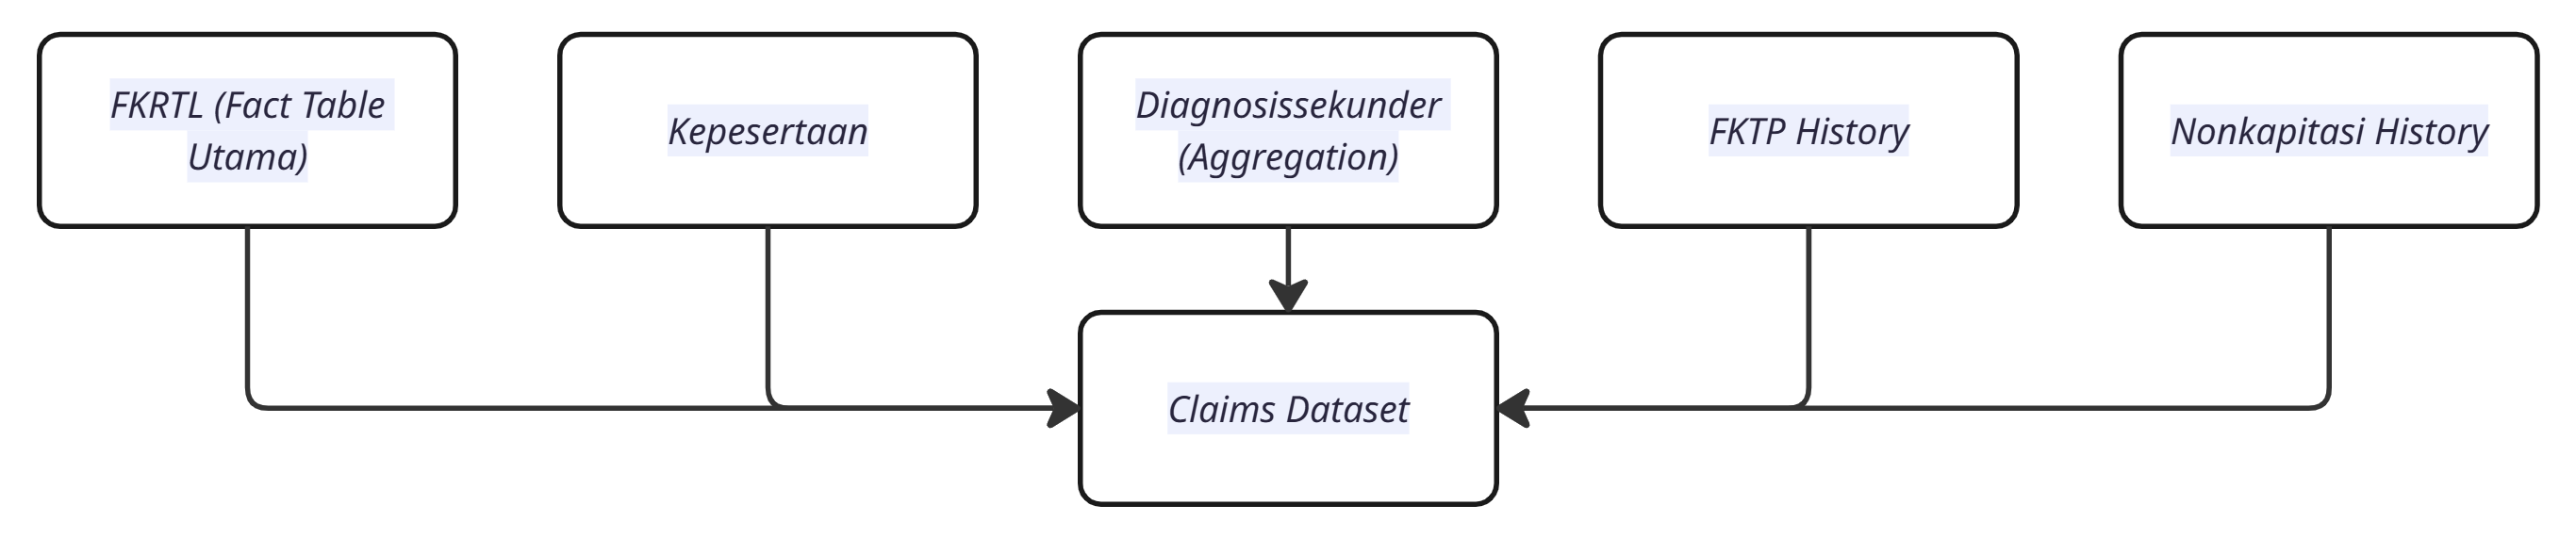
\includegraphics[width=5.51181in,height=1.15208in]{media/media/image10.png}

\phantomsection\label{_Toc228109338}{}Gambar 4. 1 Diagram Integrasi Claim-Centric

Berdasarkan Gambar 4.1, alur integrasi dimulai dari~FKRTL~sebagai pusat analisis, lalu diperkaya melalui integrasi atribut~kepesertaan, agregasi~diagnosissekunder, serta pembentukan histori layanan dari~FKTP~dan~nonkapitasi. Hasil akhir dari tahapan tersebut adalah terbentuknya~claims dataset, yaitu dataset analitis pada level klaim yang siap digunakan untuk proses pembersihan lanjutan, pembentukan fitur, dan pemodelan.

Untuk memperjelas sumber variabel yang masuk ke dalam proses integrasi, ringkasan asal data, variabel yang diambil, dan hasil integrasinya ditunjukkan pada Tabel 4.11.

\phantomsection\label{_Toc228109416}{}Tabel 4. 11 Ringkasan Integrasi Claim-Centric

\begin{longtable}[]{@{}
  >{\raggedright\arraybackslash}p{(\columnwidth - 4\tabcolsep) * \real{0.2510}}
  >{\raggedright\arraybackslash}p{(\columnwidth - 4\tabcolsep) * \real{0.4427}}
  >{\raggedright\arraybackslash}p{(\columnwidth - 4\tabcolsep) * \real{0.3063}}@{}}
\toprule\noalign{}
\begin{minipage}[b]{\linewidth}\raggedright
\textbf{Sumber}
\end{minipage} & \begin{minipage}[b]{\linewidth}\raggedright
\textbf{Variabel yang Diambil}
\end{minipage} & \begin{minipage}[b]{\linewidth}\raggedright
\textbf{Hasil Integrasi}
\end{minipage} \\
\midrule\noalign{}
\endhead
\bottomrule\noalign{}
\endlastfoot
fkrtl & id\_klaim,~id\_peserta, tanggal layanan, tarif, severity, atribut klaim utama & Menjadi struktur dasar dataset klaim \\
kepesertaan & jenis kelamin, tanggal lahir, status kepesertaan, atribut peserta & Menambah konteks peserta pada klaim \\
diagnosissekunder & kode diagnosis sekunder, grup diagnosis sekunder & Membentuk agregasi diagnosis sekunder per klaim \\
fktpkapitasi & tanggal pelayanan dan riwayat kunjungan FKTP & Membentuk fitur histori layanan FKTP \\
nonkapitasi & tanggal pelayanan dan biaya layanan nonkapitasi & Membentuk fitur histori layanan dan biaya nonkapitasi \\
\end{longtable}

Tabel 4.11 memperlihatkan bahwa setiap sumber data menyumbang informasi yang berbeda ke dalam struktur akhir klaim.~fkrtl~menyumbang identitas klaim dan komponen inti pelayanan,~kepesertaan~menyumbang atribut peserta,~diagnosissekunder~menyumbang ringkasan diagnosis tambahan, sedangkan~fktpkapitasi~dan~nonkapitasi~menyumbang histori layanan peserta sebelum klaim terjadi. Dengan susunan seperti ini, dataset hasil integrasi tidak hanya kaya secara informasi, tetapi juga tetap konsisten karena seluruh pengayaan dilakukan di sekitar unit analisis yang sama, yaitu klaim.

\subsection{Karakteristik Variabel dan Feature Engineering}\label{karakteristik-variabel-dan-feature-engineering}

Setelah integrasi data selesai dilakukan, tahapan berikutnya adalah pembentukan fitur yang digunakan untuk eksperimen. Fitur-fitur pada penelitian ini tidak dibangun secara acak, tetapi disusun ke dalam beberapa kelompok besar berdasarkan fungsi analitisnya, yaitu fitur demografis, biaya, klinis, diagnosis, histori layanan, dan rasio turunan. Pengelompokan ini penting karena setiap kelompok fitur mewakili dimensi yang berbeda dalam membaca karakteristik klaim.

Fitur demografis digunakan untuk merepresentasikan profil dasar peserta, seperti usia dan jenis kelamin. Fitur biaya digunakan untuk menangkap besaran finansial klaim, baik dalam bentuk nilai absolut maupun biaya turunan. Fitur klinis digunakan untuk menggambarkan tingkat keparahan pelayanan dan karakteristik perawatan. Sementara itu, fitur diagnosis digunakan untuk menangkap intensitas diagnosis sekunder, fitur histori layanan digunakan untuk merekam pola utilisasi sebelum klaim, dan rasio turunan digunakan untuk menyoroti ketidakwajaran relatif antar komponen biaya dan histori layanan.

Untuk memberikan gambaran awal mengenai karakteristik dataset, penelitian ini menampilkan distribusi empat variabel numerik utama, yaitu~usia,~lama\_rawat\_hari,~severity\_level, dan~tarif\_disetujui. Keempat variabel tersebut dipilih karena mewakili dimensi penting dalam data klaim, yaitu profil peserta, karakteristik pelayanan klinis, tingkat keparahan kasus, dan besaran finansial klaim.

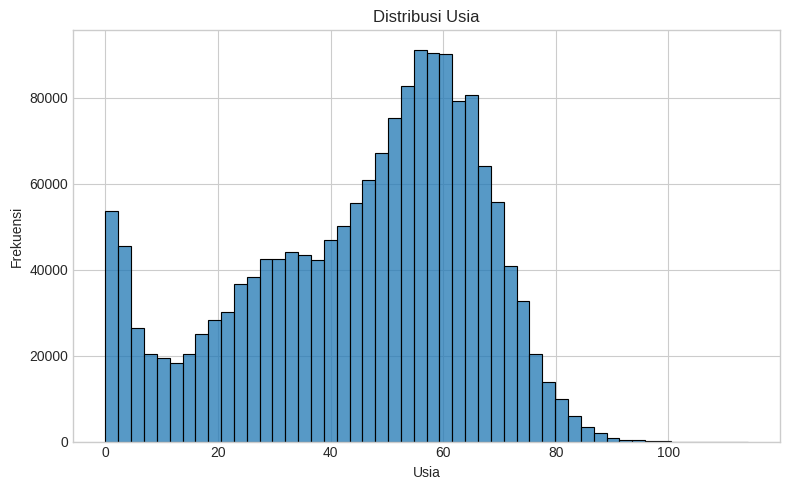
\includegraphics[width=5.51181in,height=3.41736in]{media/media/image11.png}

\phantomsection\label{_Toc228109339}{}Gambar 4. 2 Distribusi Usia

Distribusi~usia~ditunjukkan pada~Gambar 4.2. Gambar tersebut memperlihatkan bahwa data mencakup rentang usia yang luas, sehingga profil peserta pada dataset tidak terkonsentrasi hanya pada satu kelompok umur tertentu. Sebaran ini menunjukkan bahwa model perlu menangani variasi karakteristik peserta yang cukup beragam pada level klaim.

Distribusi~lama\_rawat\_hari~ditunjukkan pada~Gambar 4.3. Berdasarkan gambar tersebut, durasi rawat cenderung terkonsentrasi pada nilai yang lebih rendah, namun tetap memiliki ekor distribusi yang panjang. Pola ini menunjukkan bahwa sebagian besar klaim berkaitan dengan lama rawat yang singkat, sementara sebagian lainnya memiliki durasi yang jauh lebih panjang dan berpotensi memberikan sinyal klinis maupun finansial yang berbeda.

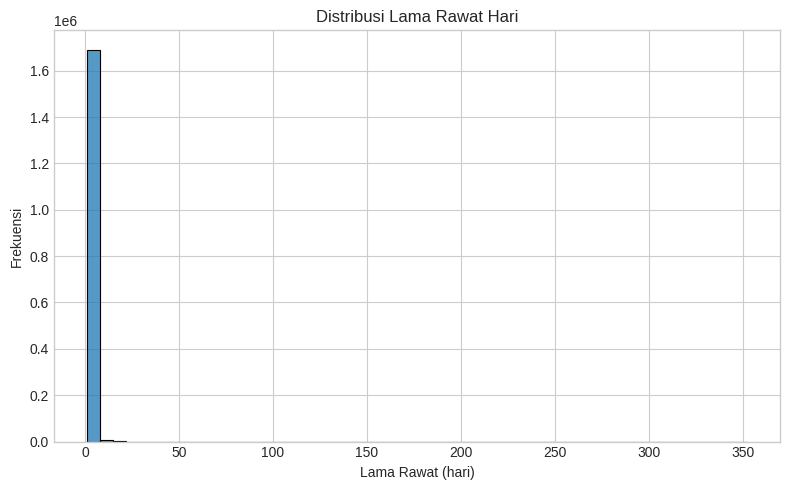
\includegraphics[width=5.51181in,height=3.41736in]{media/media/image12.png}

\phantomsection\label{_Toc228109340}{}Gambar 4. 3 Distribusi Lama Rawat Hari

Distribusi~severity\_level~ditunjukkan pada~Gambar 4.4. Variabel ini penting karena merepresentasikan tingkat keparahan kasus pada klaim. Sebaran pada gambar tersebut menunjukkan bahwa tingkat keparahan tidak homogen, sehingga model perlu mempertimbangkan variasi kompleksitas kasus sebagai salah satu unsur penting dalam membaca kewajaran klaim.

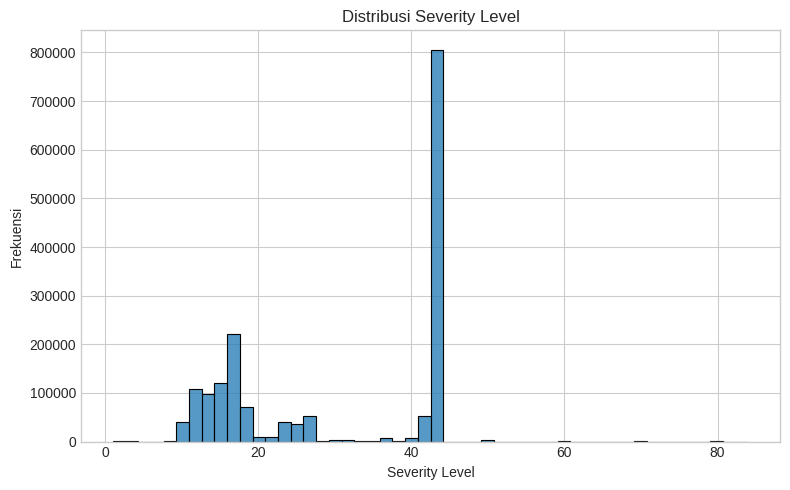
\includegraphics[width=5.51181in,height=3.41736in]{media/media/image13.png}

\phantomsection\label{_Toc228109341}{}Gambar 4. 4 Distribusi Severity Level

Distribusi~tarif\_disetujui~ditunjukkan pada~Gambar 4.5. Gambar tersebut memperlihatkan bahwa nilai biaya klaim memiliki rentang yang sangat lebar, dengan sebagian klaim berada pada kisaran biaya yang jauh lebih tinggi daripada Meioritas populasi. Variasi finansial yang besar ini menunjukkan bahwa komponen biaya memiliki posisi penting dalam eksperimen, terutama pada tahap pseudo-labeling dan seleksi fitur, karena pola anomali biaya berpotensi menjadi salah satu penanda utama klaim berisiko.

Secara keseluruhan, keempat distribusi tersebut menunjukkan bahwa dataset pada penelitian ini memiliki keragaman yang cukup besar dari sisi peserta, pelayanan, keparahan klinis, dan nilai finansial. Karakteristik inilah yang kemudian menjadi dasar penting dalam pembentukan pseudo-label, preprocessing, dan pemilihan konfigurasi fitur pada tahap pemodelan.

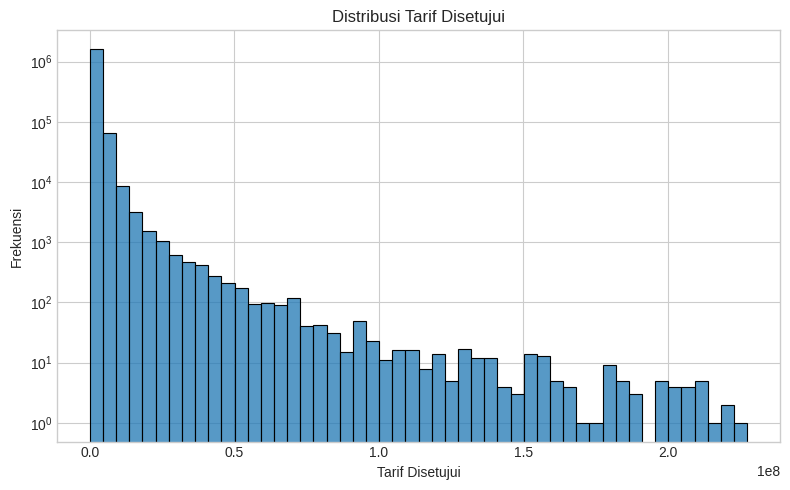
\includegraphics[width=5.51181in,height=3.41736in]{media/media/image14.png}

\phantomsection\label{_Toc228109342}{}Gambar 4. 5 Distribusi Tarif Disetujui

Untuk memperjelas susunan kelompok fitur yang digunakan pada dataset akhir, ringkasan kelompok fitur beserta contoh variabel dan tujuan analitisnya disajikan pada Tabel 4.12.

\phantomsection\label{_Toc228109417}{}Tabel 4. 12 Kelompok Fitur Final

\begin{longtable}[]{@{}
  >{\raggedright\arraybackslash}p{(\columnwidth - 4\tabcolsep) * \real{0.2498}}
  >{\raggedright\arraybackslash}p{(\columnwidth - 4\tabcolsep) * \real{0.4168}}
  >{\raggedright\arraybackslash}p{(\columnwidth - 4\tabcolsep) * \real{0.3334}}@{}}
\toprule\noalign{}
\begin{minipage}[b]{\linewidth}\raggedright
\textbf{Kelompok Fitur}
\end{minipage} & \begin{minipage}[b]{\linewidth}\raggedright
\textbf{Contoh Variabel}
\end{minipage} & \begin{minipage}[b]{\linewidth}\raggedright
\textbf{Tujuan Analitis}
\end{minipage} \\
\midrule\noalign{}
\endhead
\bottomrule\noalign{}
\endlastfoot
Demografis & usia,~gender\_singkat & Menggambarkan profil dasar peserta \\
Biaya & tarif\_disetujui,~tarif\_inacbg\_dasar,~biaya\_per\_hari & Menangkap pola finansial klaim \\
Klinis & severity\_level,~lama\_rawat\_hari,~total\_special\_cmg & Menggambarkan tingkat keparahan dan karakteristik layanan \\
Diagnosis & jumlah\_diagnosis\_sekunder,~jumlah\_grup\_diagnosis\_sekunder & Mengukur intensitas diagnosis tambahan \\
Histori layanan & fktp\_hist\_count\_before,~nonkap\_hist\_count\_before & Menangkap pola utilisasi sebelum klaim \\
Rasio turunan & rasio\_tarif\_setuju\_vs\_dasar,~rasio\_biaya\_klaim\_vs\_histori\_nonkap & Menyoroti hubungan relatif antar komponen biaya dan histori \\
\end{longtable}

Tabel 4.12 menunjukkan bahwa setiap kelompok fitur memiliki peran analitis yang berbeda. Fitur demografis membantu membaca konteks peserta, fitur biaya menggambarkan beban finansial klaim, fitur klinis memperlihatkan tingkat keparahan dan karakteristik pelayanan, fitur diagnosis menangkap intensitas kondisi tambahan, fitur histori layanan memberikan konteks utilisasi sebelum klaim, dan rasio turunan membantu menilai hubungan relatif antar komponen biaya dan riwayat layanan. Dengan pengelompokan tersebut, dataset akhir pada penelitian ini tidak hanya kaya secara jumlah fitur, tetapi juga kaya secara makna analitis.

\subsection{Implikasi Karakteristik Data terhadap Eksperimen}\label{implikasi-karakteristik-data-terhadap-eksperimen}

Karakteristik data yang telah dijelaskan pada subbab sebelumnya memiliki implikasi langsung terhadap pembentukan model. Salah satu implikasi utama adalah munculnya ketidakseimbangan label setelah tahap pseudo-labeling. Karena klaim yang ditandai sebagai anomali hanya merupakan sebagian kecil dari keseluruhan populasi, maka model harus dibangun pada kondisi distribusi kelas yang tidak seimbang. Kondisi ini berpengaruh pada pemilihan metrik evaluasi, teknik preprocessing, serta kebutuhan~\emph{threshold tuning}~pada tahap akhir.

Implikasi berikutnya adalah besarnya variasi nilai biaya antar klaim. Variabel seperti~tarif\_disetujui~dan komponen biaya lainnya menunjukkan rentang yang sangat lebar, sehingga tanpa preprocessing yang tepat, model dapat terdorong terlalu kuat oleh variabel biaya mentah. Oleh karena itu, transformasi numerik, pembentukan rasio turunan, dan mekanisme seleksi fitur menjadi penting agar model tidak hanya sensitif terhadap besaran biaya absolut, tetapi juga terhadap pola ketidakwajaran yang lebih informatif.

Karakteristik data juga menunjukkan bahwa histori layanan memiliki posisi penting dalam eksperimen. Kehadiran fitur histori dari~fktpkapitasi~dan~nonkapitasi~memungkinkan model tidak hanya membaca klaim sebagai transaksi tunggal, tetapi juga sebagai bagian dari riwayat pemanfaatan layanan peserta. Dengan adanya konteks historis tersebut, model memiliki dasar yang lebih kuat untuk membedakan klaim yang memang tinggi karena pola pelayanan sebelumnya dengan klaim yang tampak menyimpang secara tidak wajar.

Selain itu, kompleksitas struktur data yang terbentuk dari integrasi multi-tabel membuat tahap preprocessing dan~\emph{feature selection}~menjadi keharusan, bukan pelengkap. Banyaknya fitur dengan tipe yang berbeda, kemungkinan redundansi antarvariabel, serta potensi multikolinearitas menjadikan proses seleksi fitur sebagai bagian penting dalam eksperimen. Dengan kata lain, karakteristik data pada penelitian ini secara langsung menjelaskan mengapa eksperimen memerlukan tahapan split yang terkontrol, preprocessing yang sistematis, dan beberapa~\emph{branch feature selection}~sebelum masuk ke tahap benchmarking model.

Secara keseluruhan, karakteristik data pada penelitian ini membentuk dasar teknis bagi seluruh eksperimen yang dilakukan. Struktur data yang kaya, skala data yang besar, variasi biaya yang tinggi, serta distribusi label yang tidak seimbang menjadikan eksperimen tidak dapat dilakukan dengan pendekatan klasifikasi sederhana. Justru karena karakteristik data itulah, pipeline final pada penelitian ini dirancang dalam bentuk integrasi berbasis klaim, pseudo-labeling, seleksi fitur bertingkat, benchmarking multi-model, dan evaluasi yang dilengkapi interpretabilitas.

\section{TEMPAT UJI COBA}\label{tempat-uji-coba}

Subbab ini menjelaskan lingkungan tempat eksperimen dijalankan. Penjelasan mengenai tempat ujicoba diperlukan agar pelaksanaan eksperimen dapat dipahami dalam konteks lingkungan komputasi yang digunakan, termasuk platform notebook, ruang kerja eksekusi, dan lokasi penyimpanan artefak hasil. Dengan mencantumkan lingkungan ujicoba secara jelas, hasil eksperimen pada penelitian ini dapat dibaca sebagai keluaran dari proses yang dijalankan pada satu lingkungan komputasi yang konsisten.

Eksperimen pada penelitian ini dijalankan pada platform komputasi berbasis notebook dengan lingkungan kerja Python yang mendukung proses pengolahan data, pemodelan, evaluasi, dan interpretabilitas. Lingkungan tersebut memungkinkan seluruh pipeline dijalankan secara terintegrasi, mulai dari pembacaan tabel mentah, pembentukan dataset berbasis klaim, pelaksanaan benchmarking model, hingga penyimpanan artefak hasil eksperimen. Dengan demikian, tempat ujicoba pada penelitian ini tidak dipahami sebagai lokasi fisik semata, tetapi sebagai lingkungan komputasi tempat seluruh eksperimen dijalankan.

Lingkungan notebook yang digunakan juga berperan sebagai ruang kerja utama selama eksperimen berlangsung. Seluruh tahapan analisis dilakukan di dalam notebook yang sama, sehingga alur eksperimen dapat dijalankan secara runtut dan terdokumentasi dengan baik. Hal ini penting karena pipeline penelitian ini tidak terdiri atas satu tahap tunggal, melainkan serangkaian proses yang saling terkait dari awal sampai akhir.

Selain sebagai tempat eksekusi, lingkungan ujicoba pada penelitian ini juga menjadi lokasi keluaran artefak eksperimen. Artefak seperti informasi model pemenang, analisis threshold, hasil evaluasi akhir, dan keluaran interpretabilitas disimpan pada direktori kerja notebook, sehingga dapat digunakan kembali untuk kebutuhan pelaporan dan analisis lanjutan. Ringkasan komponen lingkungan ujicoba yang digunakan pada penelitian ini ditunjukkan pada Tabel 4.13.

\phantomsection\label{_Toc228109418}{}Tabel 4. 13 Lingkungan Uji Coba

\begin{longtable}[]{@{}
  >{\raggedright\arraybackslash}p{(\columnwidth - 2\tabcolsep) * \real{0.2538}}
  >{\raggedright\arraybackslash}p{(\columnwidth - 2\tabcolsep) * \real{0.7462}}@{}}
\toprule\noalign{}
\begin{minipage}[b]{\linewidth}\raggedright
\textbf{Komponen}
\end{minipage} & \begin{minipage}[b]{\linewidth}\raggedright
\textbf{Deskripsi}
\end{minipage} \\
\midrule\noalign{}
\endhead
\bottomrule\noalign{}
\endlastfoot
Platform komputasi & Lingkungan komputasi berbasis notebook cloud \\
Lingkungan notebook & Notebook Python yang digunakan untuk menjalankan seluruh pipeline eksperimen \\
Lokasi output artefak & Hasil pekerjaan disimpan dalam bentul Notebook .ipynb di platform Kaggle \\
\end{longtable}

Berdasarkan Tabel 4.13, lingkungan ujicoba pada penelitian ini terdiri atas tiga komponen utama, yaitu platform komputasi, lingkungan notebook, dan lokasi penyimpanan artefak hasil. Platform komputasi berfungsi sebagai tempat pelaksanaan seluruh eksperimen, lingkungan notebook berfungsi sebagai ruang kerja interaktif untuk menjalankan pipeline, sedangkan direktori keluaran artefak menjadi lokasi penyimpanan hasil eksperimen yang dihasilkan selama proses analisis. Dengan susunan tersebut, eksperimen pada penelitian ini dijalankan dalam lingkungan yang terpusat dan konsisten, sehingga seluruh keluaran dapat ditelusuri kembali dengan lebih mudah.

\section{WAKTU UJI COBA}\label{waktu-uji-coba}

Subbab ini menjelaskan waktu pelaksanaan eksperimen dan rerun final yang dijadikan dasar hasil pada Bab 4. Penjelasan waktu ujicoba penting untuk menegaskan bahwa hasil yang dibahas pada bab ini tidak diambil secara acak dari beberapa versi eksperimen yang berbeda, melainkan berasal dari satu pelaksanaan final yang dijadikan acuan utama.

Pelaksanaan eksperimen pada penelitian ini berlangsung pada tahap pengolahan data, pemodelan, evaluasi, dan interpretabilitas dalam lingkungan notebook final. Dari keseluruhan proses tersebut, hasil yang digunakan sebagai dasar penulisan Bab 4 diturunkan dari rerun final notebook yang menghasilkan keluaran eksperimen lengkap dan artefak hasil yang konsisten. Penetapan rerun final sebagai acuan utama diperlukan agar semua angka, tabel, dan pembahasan pada bab ini berasal dari satu konfigurasi eksperimen yang sama.

Waktu rerun final menjadi penanda penting karena menunjukkan titik ketika pipeline telah dijalankan dengan konfigurasi akhir yang stabil. Dengan demikian, hasil pada Bab 4 merepresentasikan kondisi akhir eksperimen yang digunakan dalam penelitian ini, bukan keluaran antara atau percobaan awal yang belum final. Ringkasan tahapan waktu pelaksanaan ujicoba dan rerun final yang digunakan sebagai dasar hasil Bab 4 ditunjukkan pada Tabel 4.14.

\phantomsection\label{_Toc228109419}{}Tabel 4. 14 Waktu Pelaksanaan Uji Coba

\begin{longtable}[]{@{}
  >{\raggedright\arraybackslash}p{(\columnwidth - 4\tabcolsep) * \real{0.2378}}
  >{\raggedright\arraybackslash}p{(\columnwidth - 4\tabcolsep) * \real{0.4049}}
  >{\raggedright\arraybackslash}p{(\columnwidth - 4\tabcolsep) * \real{0.3573}}@{}}
\toprule\noalign{}
\begin{minipage}[b]{\linewidth}\raggedright
\textbf{Tahap}
\end{minipage} & \begin{minipage}[b]{\linewidth}\raggedright
\textbf{Waktu Pelaksanaan}
\end{minipage} & \begin{minipage}[b]{\linewidth}\raggedright
\textbf{Keterangan}
\end{minipage} \\
\midrule\noalign{}
\endhead
\bottomrule\noalign{}
\endlastfoot
Persiapan eksperimen & Periode pengolahan data dan penyusunan pipeline & Mencakup integrasi data dan rekayasa fitur \\
Pelaksanaan eksperimen & Periode benchmarking, evaluasi, dan interpretabilitas & Mencakup seluruh tahapan pengujian model \\
Rerun final notebook & 17 April 2026 & Menjadi dasar hasil yang digunakan pada Bab 4 \\
\end{longtable}

Tabel 4.14 menunjukkan bahwa pelaksanaan eksperimen pada penelitian ini dapat dibedakan ke dalam tahap persiapan eksperimen, pelaksanaan pipeline, dan rerun final yang dijadikan dasar penulisan hasil. Keberadaan kolom keterangan pada tabel tersebut penting karena memberikan konteks terhadap masing-masing tahap, terutama untuk menegaskan bahwa pembahasan pada Bab 4 diturunkan dari rerun final, bukan dari hasil uji coba sementara. Dengan demikian, pembaca dapat memahami bahwa hasil yang dibahas pada bab ini memiliki titik acuan waktu yang jelas dan konsisten.

\section{SPESIFIKASI PERALATAN UJI COBA}\label{spesifikasi-peralatan-uji-coba}

Subbab ini menjelaskan perangkat keras, perangkat lunak, dan pustaka utama yang digunakan selama eksperimen. Penjelasan ini diperlukan agar pembaca memperoleh gambaran yang jelas mengenai perangkat dan lingkungan teknis yang mendukung pelaksanaan pipeline penelitian, mulai dari pengolahan data sampai interpretabilitas model.

Eksperimen pada penelitian ini dijalankan pada lingkungan notebook komputasi berbasis Python. Karena pelaksanaan eksperimen dilakukan pada platform notebook, maka spesifikasi peralatan pada penelitian ini dijelaskan dalam bentuk lingkungan komputasi yang digunakan, bahasa pemrograman, serta pustaka-pustaka utama yang benar-benar dipakai dalam pipeline. Dengan pendekatan tersebut, penjelasan spesifikasi peralatan tetap relevan terhadap proses eksperimen yang dijalankan.

Dari sisi perangkat lunak, bahasa pemrograman utama yang digunakan adalah Python dengan lingkungan notebook interaktif. Lingkungan ini mendukung proses pembacaan data, transformasi, pembentukan fitur, pelatihan model, evaluasi metrik, visualisasi, dan interpretabilitas hasil. Struktur seperti ini membuat seluruh tahapan penelitian dapat dijalankan dalam satu lingkungan kerja yang terintegrasi.

Dari sisi pustaka, eksperimen ini memanfaatkan beberapa kelompok library utama. Library pengolahan data digunakan untuk membaca, membersihkan, dan mentransformasikan data tabular. Library pemodelan digunakan untuk menjalankan pseudo-labeling, preprocessing, benchmarking model, dan evaluasi performa. Sementara itu, library interpretabilitas digunakan untuk menjelaskan keluaran model pada tingkat global maupun lokal. Ringkasan spesifikasi peralatan ujicoba yang digunakan pada penelitian ini ditunjukkan pada Tabel 4.15.

\phantomsection\label{_Toc228109420}{}Tabel 4. 15 Spesifikasi Peralatan Uji Coba

\begin{longtable}[]{@{}
  >{\raggedright\arraybackslash}p{(\columnwidth - 4\tabcolsep) * \real{0.2498}}
  >{\raggedright\arraybackslash}p{(\columnwidth - 4\tabcolsep) * \real{0.3218}}
  >{\raggedright\arraybackslash}p{(\columnwidth - 4\tabcolsep) * \real{0.4284}}@{}}
\toprule\noalign{}
\begin{minipage}[b]{\linewidth}\raggedright
\textbf{Komponen}
\end{minipage} & \begin{minipage}[b]{\linewidth}\raggedright
\textbf{Spesifikasi}
\end{minipage} & \begin{minipage}[b]{\linewidth}\raggedright
\textbf{Fungsi}
\end{minipage} \\
\midrule\noalign{}
\endhead
\bottomrule\noalign{}
\endlastfoot
Perangkat komputasi & Lingkungan notebook cloud & Menjalankan seluruh proses eksperimen \\
Bahasa pemrograman & Python & Bahasa utama untuk pengolahan data dan pemodelan \\
Lingkungan kerja & Jupyter Notebook / Kaggle Notebook & Menjalankan pipeline secara interaktif \\
Library pengolahan data & pandas,~numpy & Membaca, membersihkan, dan mentransformasikan data \\
Library visualisasi & matplotlib,~seaborn & Membuat grafik dan visualisasi eksperimen \\
Library pemodelan & scikit-learn,~xgboost,~lightgbm,~catboost & Menjalankan pseudo-labeling, preprocessing, benchmarking, dan evaluasi \\
Library interpretabilitas & shap,~lime & Menjelaskan hasil prediksi model \\
Library tambahan & optuna~atau library tuning lain jika dipakai & Mendukung optimasi parameter model \\
\end{longtable}

Berdasarkan Tabel 4.15, spesifikasi peralatan ujicoba pada penelitian ini dapat dibaca sebagai kombinasi antara lingkungan komputasi notebook, bahasa pemrograman Python, serta pustaka-pustaka utama yang mendukung setiap tahap eksperimen. Komponen untuk pengolahan data berfungsi membentuk dataset analitis yang siap dipakai, komponen pemodelan berfungsi menjalankan pseudo-labeling dan benchmarking model, sedangkan komponen interpretabilitas berfungsi membaca dan menjelaskan keputusan model. Dengan konfigurasi seperti ini, seluruh tahapan eksperimen dapat dilaksanakan secara terpadu dalam satu lingkungan kerja yang konsisten.

\section{HASIL EKSPERIMEN}\label{hasil-eksperimen}

Subbab ini menyajikan hasil eksperimen yang diperoleh dari pelaksanaan pipeline final penelitian. Penyajian hasil dilakukan secara bertahap mengikuti urutan proses eksperimen, mulai dari pembentukan basis klaim, pembentukan dataset pemodelan, pseudo-labeling, pembagian data, seleksi fitur, benchmarking model, penetapan model final, evaluasi performa, interpretabilitas, hingga artefak hasil yang diekspor. Dengan susunan seperti ini, pembaca dapat mengikuti keluaran eksperimen secara runtut dari tahap awal hingga tahap akhir.

Berbeda dari pembahasan parameter eksperimen pada subbab sebelumnya, bagian ini berfokus pada keluaran aktual yang dihasilkan dari pipeline. Setiap subbagian pada 4.6 mewakili satu keluaran utama, sehingga hubungan antara tahapan eksperimen dan hasil yang diperoleh dapat dibaca dengan lebih jelas. Pendekatan ini juga memudahkan pembaca untuk melihat bagaimana satu tahap memengaruhi tahap berikutnya sampai akhirnya menghasilkan model final beserta interpretasinya.

\subsection{Hasil Integrasi Claim-Centric}\label{hasil-integrasi-claim-centric}

Tahap awal eksperimen menghasilkan pembentukan basis klaim melalui integrasi data berbasis~claim-centric. Pada tahap ini,~fkrtl~digunakan sebagai kerangka utama, kemudian diperkaya dengan atribut dari~kepesertaan, agregasi dari~diagnosissekunder, serta histori layanan dari~fktpkapitasi~dan~nonkapitasi. Hasil integrasi ini menjadi fondasi bagi seluruh eksperimen karena seluruh tahapan selanjutnya dijalankan di atas dataset klaim yang telah diperkaya.

Berdasarkan hasil integrasi, jumlah observasi akhir tetap berada pada level klaim dan tidak berubah menjadi level peserta atau level kunjungan. Hal ini menunjukkan bahwa strategi integrasi yang digunakan berhasil mempertahankan satu klaim sebagai satu unit observasi utama. Dengan demikian, struktur akhir dataset tetap selaras dengan tujuan penelitian, yaitu mendeteksi potensi fraud atau upcoding pada level transaksi klaim.

Ringkasan hasil integrasi~claim-centric~ditunjukkan pada Tabel 4.16. Tabel tersebut memperlihatkan tahapan utama pembentukan basis klaim, keluaran pada setiap tahap, serta ukuran data yang dihasilkan.

\phantomsection\label{_Toc228109421}{}Tabel 4. 16 Hasil Integrasi Claim-Centric

\begin{longtable}[]{@{}
  >{\raggedright\arraybackslash}p{(\columnwidth - 4\tabcolsep) * \real{0.3333}}
  >{\raggedright\arraybackslash}p{(\columnwidth - 4\tabcolsep) * \real{0.3333}}
  >{\raggedright\arraybackslash}p{(\columnwidth - 4\tabcolsep) * \real{0.3334}}@{}}
\toprule\noalign{}
\begin{minipage}[b]{\linewidth}\raggedright
\textbf{Tahap}
\end{minipage} & \begin{minipage}[b]{\linewidth}\raggedright
\textbf{Output}
\end{minipage} & \begin{minipage}[b]{\linewidth}\raggedright
\textbf{Ukuran Data}
\end{minipage} \\
\midrule\noalign{}
\endhead
\bottomrule\noalign{}
\endlastfoot
Pemuatan~fkrtl & Basis klaim awal & 1.699.219 x 57 \\
Integrasi dengan~kepesertaan & Klaim dengan atribut peserta & sesuai hasil merge \\
Agregasi~diagnosissekunder & Klaim dengan ringkasan diagnosis sekunder & sesuai hasil agregasi \\
Integrasi histori~fktpkapitasi~dan~nonkapitasi & Klaim dengan fitur histori layanan & sesuai hasil integrasi akhir \\
Pembentukan~claims & Dataset klaim final sebelum feature engineering & 1.699.219 x 79 \\
\end{longtable}

Berdasarkan Tabel 4.16, hasil integrasi menghasilkan struktur klaim akhir yang memuat informasi peserta, diagnosis sekunder, dan histori layanan dalam satu dataset yang tetap terpusat pada klaim. Hal ini penting karena kualitas tahap integrasi akan menentukan kualitas fitur yang dibentuk pada tahap berikutnya. Dengan kata lain, keberhasilan eksperimen pada tahap pemodelan sangat bergantung pada keberhasilan pembentukan basis klaim pada tahap ini.

\subsection{Hasil Feature Engineering dan Modeling Dataset}\label{hasil-feature-engineering-dan-modeling-dataset}

Setelah basis klaim terbentuk, eksperimen dilanjutkan ke tahap~\emph{feature engineering}~untuk membangun variabel yang digunakan pada pemodelan. Pada tahap ini, fitur akhir dibentuk dari kombinasi informasi administratif, klinis, biaya, diagnosis, serta histori layanan. Hasil pembentukan fitur tersebut kemudian dihimpun ke dalam~model\_df, yaitu dataset pemodelan yang menjadi dasar seluruh tahap eksperimen selanjutnya.

Hasil eksperimen menunjukkan bahwa model\_df berhasil dibentuk dengan ukuran yang besar dan mencakup fitur-fitur yang dibutuhkan untuk tahap unsupervised maupun supervised. Struktur ini penting karena model\_df menjadi titik pertemuan antara hasil integrasi data, rekayasa fitur, dan kebutuhan pemodelan, sehingga kualitas serta kelengkapan fitur pada tahap ini sangat menentukan kualitas pseudo-labeling dan proses benchmarking berikutnya.

Tabel 4.17 menunjukkan bahwa dataset pemodelan akhir terdiri atas 1.699.219 observasi dengan 51 kolom, 14 fitur unsupervised, dan seperangkat fitur supervised final yang digunakan pada tahap klasifikasi. Susunan ini menunjukkan bahwa hasil feature engineering tidak hanya memperkaya data klaim, tetapi juga menghasilkan struktur dataset yang siap dipakai secara langsung untuk membangun target awal, melatih model, dan mengevaluasi performa.

Untuk memperjelas hasil pembentukan dataset pemodelan, ringkasan komponen utama~model\_df~ditunjukkan pada Tabel 4.17.

\phantomsection\label{_Toc228109422}{}Tabel 4. 17 Ringkasan Modeling Dataset

\begin{longtable}[]{@{}
  >{\raggedright\arraybackslash}p{(\columnwidth - 2\tabcolsep) * \real{0.4997}}
  >{\raggedright\arraybackslash}p{(\columnwidth - 2\tabcolsep) * \real{0.5003}}@{}}
\toprule\noalign{}
\begin{minipage}[b]{\linewidth}\raggedright
\textbf{Komponen}
\end{minipage} & \begin{minipage}[b]{\linewidth}\raggedright
\textbf{Nilai}
\end{minipage} \\
\midrule\noalign{}
\endhead
\bottomrule\noalign{}
\endlastfoot
Jumlah observasi & 1.699.219 \\
Jumlah kolom~model\_df & 51 \\
Jumlah fitur unsupervised & 14 \\
Jumlah fitur supervised & sesuai daftar final \\
Unit analisis & Satu klaim \\
\end{longtable}

Tabel 4.17 menunjukkan ukuran dataset pemodelan, jumlah fitur yang dihimpun, serta peran~model\_df~sebagai dasar bagi tahap pseudo-labeling dan supervised learning. Dengan tersusunnya~model\_df, eksperimen pada penelitian ini memasuki tahap pemodelan dengan satu dataset akhir yang telah siap dipakai secara langsung.

Dengan terbentuknya model\_df, eksperimen pada penelitian ini memasuki tahap pemodelan dengan satu dataset akhir yang telah terintegrasi, bersih, dan relevan secara analitis. Oleh karena itu, hasil pada subbab ini menegaskan bahwa tahap feature engineering berhasil mengubah data klaim multi-sumber menjadi dataset pemodelan yang operasional untuk seluruh pipeline penelitian.

\subsection{Hasil Pseudo-Labeling dengan Isolation Forest}\label{hasil-pseudo-labeling-dengan-isolation-forest}

Setelah dataset pemodelan terbentuk, eksperimen dilanjutkan ke tahap pseudo-labeling menggunakan~Isolation Forest. Tahap ini dilakukan untuk membentuk target awal pada data yang semula tidak memiliki label fraud aktual. Pseudo-labeling menjadi penting karena tanpa target awal, eksperimen tidak dapat dilanjutkan ke tahap supervised benchmarking.

Hasil sensitivity analysis terhadap beberapa nilai~contamination rate~menunjukkan bahwa jumlah klaim yang ditandai sebagai anomali berubah secara proporsional terhadap nilai kontaminasi yang diuji. Pada tingkat~0,01, jumlah klaim anomali berada pada kisaran terendah, sedangkan pada tingkat~0,10, jumlah klaim anomali meningkat jauh lebih besar. Variasi ini menunjukkan bahwa hasil pseudo-labeling sensitif terhadap asumsi proporsi anomali, sehingga pemilihan konfigurasi final perlu dilakukan secara hati-hati.

Hasil pseudo-labeling pada konfigurasi final menunjukkan bahwa jumlah klaim yang diberi label berisiko berada pada proporsi kecil dibandingkan total populasi klaim. Kondisi ini memperlihatkan bahwa pseudo-label yang terbentuk memang merepresentasikan anomali sebagai kelompok minoritas, sesuai dengan karakter umum fraud detection. Ringkasan hasil sensitivity pseudo-labeling ditunjukkan pada Tabel 4.18.

\phantomsection\label{_Toc228109423}{}Tabel 4. 18 Sensitivity Pseudo-Labeling

\begin{longtable}[]{@{}
  >{\raggedright\arraybackslash}p{(\columnwidth - 6\tabcolsep) * \real{0.3211}}
  >{\raggedright\arraybackslash}p{(\columnwidth - 6\tabcolsep) * \real{0.2680}}
  >{\raggedright\arraybackslash}p{(\columnwidth - 6\tabcolsep) * \real{0.1608}}
  >{\raggedright\arraybackslash}p{(\columnwidth - 6\tabcolsep) * \real{0.2501}}@{}}
\toprule\noalign{}
\begin{minipage}[b]{\linewidth}\raggedright
\textbf{Contamination Rate}
\end{minipage} & \begin{minipage}[b]{\linewidth}\raggedright
\textbf{Jumlah Anomali}
\end{minipage} & \begin{minipage}[b]{\linewidth}\raggedright
\textbf{Rasio}
\end{minipage} & \begin{minipage}[b]{\linewidth}\raggedright
\textbf{Median Score}
\end{minipage} \\
\midrule\noalign{}
\endhead
\bottomrule\noalign{}
\endlastfoot
0,01 & 16.993 & 0,01 & 0,370421 \\
0,03 & 50.977 & 0,03 & 0,370421 \\
0,05 & 84.961 & 0,05 & 0,370421 \\
0,10 & 169.922 & 0,10 & 0,370421 \\
\end{longtable}

Berdasarkan Tabel 4.18, nilai~contamination rate~sebesar~0,03~menghasilkan sekitar~50.977~klaim anomali dengan rasio sekitar~3\%~dari total populasi. Hasil ini memperlihatkan bahwa distribusi label akhir bersifat tidak seimbang, dengan Meioritas klaim berada pada kelas normal. Kondisi tersebut menjadi salah satu karakter utama data yang akan memengaruhi pemilihan metrik evaluasi dan perlunya threshold tuning pada tahap berikutnya.

Selain jumlah anomali, eksperimen ini juga membandingkan profil median antara klaim normal dan klaim yang diberi pseudo-label berisiko. Perbandingan tersebut memberikan gambaran awal mengenai karakteristik yang membedakan kedua kelompok. Profil median pseudo-label ditunjukkan pada Gambar 4.6.

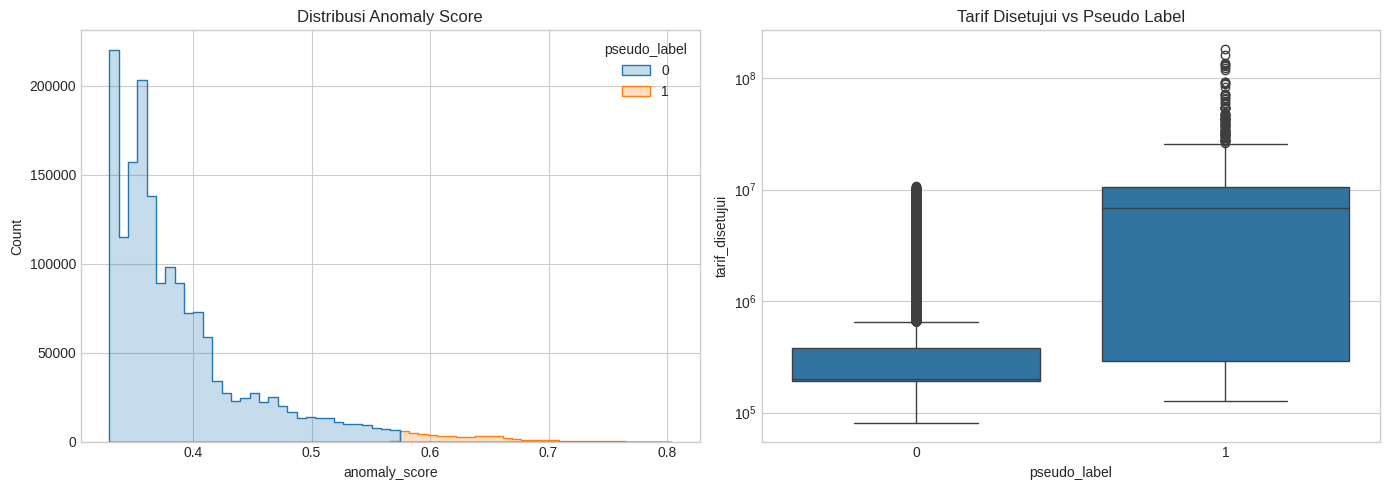
\includegraphics[width=5.51181in,height=1.94306in]{media/media/image15.png}

\phantomsection\label{_Toc228109343}{}Gambar 4. 6 Profil Median Pseudo-Label

Berdasarkan Gambar 4.6, klaim yang masuk ke kelompok~suspicious~cenderung memiliki nilai median yang lebih tinggi pada variabel biaya dan beberapa indikator layanan dibandingkan kelompok~normal. Perbedaan median ini menunjukkan bahwa pseudo-label yang terbentuk bukan bersifat acak, melainkan memiliki pola yang cukup jelas dalam membedakan klaim menyimpang dan klaim normal.

\subsection{Hasil Train/Validation/Test Split dan Preprocessing}\label{hasil-trainvalidationtest-split-dan-preprocessing}

Setelah pseudo-label dibentuk, dataset dibagi ke dalam tiga subset utama, yaitu~train,~validation, dan~test. Hasil pembagian data menunjukkan bahwa ukuran masing-masing subset sesuai dengan konfigurasi eksperimen dan distribusi label tetap terjaga secara konsisten antar subset. Hal ini penting untuk memastikan bahwa proses pelatihan, validasi, dan evaluasi berlangsung pada distribusi kelas yang sebanding.

Hasil eksperimen menunjukkan bahwa~train set~berisi~1.019.531~observasi, sedangkan~validation set~dan~test set~masing-masing berisi~339.844~observasi. Rasio pseudo-label positif pada ketiga subset tetap berada di sekitar~3\%, sehingga pembagian data dapat dikatakan berhasil mempertahankan komposisi kelas. Ringkasan hasil split dataset ditunjukkan pada Tabel 4.19.

\phantomsection\label{_Toc228109424}{}Tabel 4. 19 Hasil Split Dataset

\begin{longtable}[]{@{}
  >{\raggedright\arraybackslash}p{(\columnwidth - 4\tabcolsep) * \real{0.3333}}
  >{\raggedright\arraybackslash}p{(\columnwidth - 4\tabcolsep) * \real{0.3333}}
  >{\raggedright\arraybackslash}p{(\columnwidth - 4\tabcolsep) * \real{0.3333}}@{}}
\toprule\noalign{}
\begin{minipage}[b]{\linewidth}\raggedright
\textbf{Subset}
\end{minipage} & \begin{minipage}[b]{\linewidth}\raggedright
\textbf{Jumlah Data}
\end{minipage} & \begin{minipage}[b]{\linewidth}\raggedright
\textbf{Fraud Ratio}
\end{minipage} \\
\midrule\noalign{}
\endhead
\bottomrule\noalign{}
\endlastfoot
Train & 1.019.531 & 0,030000 \\
Validation & 339.844 & 0,030002 \\
Test & 339.844 & 0,029999 \\
\end{longtable}

Berdasarkan Tabel 4.19, konsistensi~fraud ratio~pada ketiga subset memperlihatkan bahwa proses split berjalan dengan baik dan tidak menimbulkan distorsi distribusi label. Hasil ini penting karena kestabilan distribusi kelas antar subset akan memengaruhi kualitas evaluasi model. Selain itu, tahap preprocessing yang dilakukan setelah split memastikan bahwa fitur numerik dan kategorikal dapat digunakan secara konsisten oleh seluruh model pada tahap benchmarking.

\subsection{Hasil Branch-Based Feature Selection}\label{hasil-branch-based-feature-selection}

Tahap berikutnya pada eksperimen adalah~branch-based feature selection. Pada tahap ini, beberapa strategi seleksi fitur dibandingkan untuk melihat bagaimana variasi himpunan fitur memengaruhi performa model. Eksperimen ini menghasilkan lima branch utama, yaitu domain\_expert, correlation, vif, permutation, dan~combined.

Hasil seleksi menunjukkan bahwa setiap branch menghasilkan jumlah fitur yang berbeda.~domain\_expert~menghasilkan himpunan fitur yang lebih ringkas, sedangkan~vif~menghasilkan jumlah fitur yang lebih besar dibandingkan branch lainnya.~permutation~dan~combined~menghasilkan struktur fitur yang berbeda lagi, sehingga eksperimen memiliki beberapa alternatif konfigurasi input sebelum masuk ke tahap benchmarking model.

Ringkasan hasil branch feature selection ditunjukkan pada Tabel 4.20.

\phantomsection\label{_Toc228109425}{}Tabel 4. 20 Ringkasan Branch Feature Selection

\begin{longtable}[]{@{}
  >{\raggedright\arraybackslash}p{(\columnwidth - 6\tabcolsep) * \real{0.2140}}
  >{\raggedright\arraybackslash}p{(\columnwidth - 6\tabcolsep) * \real{0.1431}}
  >{\raggedright\arraybackslash}p{(\columnwidth - 6\tabcolsep) * \real{0.3930}}
  >{\raggedright\arraybackslash}p{(\columnwidth - 6\tabcolsep) * \real{0.2500}}@{}}
\toprule\noalign{}
\begin{minipage}[b]{\linewidth}\raggedright
\textbf{Branch}
\end{minipage} & \begin{minipage}[b]{\linewidth}\raggedright
\textbf{Jumlah Fitur}
\end{minipage} & \begin{minipage}[b]{\linewidth}\raggedright
\textbf{Preview Fitur}
\end{minipage} & \begin{minipage}[b]{\linewidth}\raggedright
\textbf{Karakteristik}
\end{minipage} \\
\midrule\noalign{}
\endhead
\bottomrule\noalign{}
\endlastfoot
domain\_expert & 15 & usia, kelas\_rawat\_hak, kelas\_rawat\_klaim, stat... & Ringkas dan substantif \\
correlation & 22 & usia, regional\_tarif\_num, severity\_level, lama... & Mengurangi redundansi \\
vif & 27 & usia, regional\_tarif\_num, severity\_level, lama... & Menekan multikolinearitas \\
permutation & 20 & tarif\_grouping, nonkap\_hist\_total\_amount\_befor... & Prediktif \\
combined & 10 & fktp\_hist\_count\_before, flag\_kelas\_upgrade, fl... & Ringkas dan stabil \\
\end{longtable}

Berdasarkan Tabel 4.20, variasi jumlah fitur pada setiap branch menunjukkan bahwa strategi seleksi memang memengaruhi kompleksitas himpunan fitur yang digunakan. Tabel tersebut juga memperlihatkan contoh fitur dominan dari masing-masing branch, sehingga pembaca dapat melihat bahwa perbedaan hasil seleksi bukan hanya terletak pada jumlah fitur, tetapi juga pada karakter fitur yang dipertahankan. Dengan demikian, tahap ini menjadi dasar penting bagi proses benchmarking pada subbagian berikutnya.

\subsection{Hasil Supervised Benchmarking}\label{hasil-supervised-benchmarking}

Setelah setiap branch fitur terbentuk, eksperimen dilanjutkan ke tahap supervised benchmarking. Pada tahap ini, seluruh model dijalankan pada seluruh branch untuk menghasilkan pembandingan performa yang komprehensif. Hasil eksperimen menunjukkan bahwa kombinasi branch dan model tertentu memberikan performa yang lebih tinggi dibandingkan kombinasi lainnya.

Secara umum, model-model berbasis boosting menempati peringkat atas hasil benchmarking, terutama ketika dipadukan dengan branch yang mempertahankan fitur yang lebih informatif. Sementara itu, model linear dan beberapa konfigurasi lain menunjukkan performa yang lebih rendah. Dengan demikian, hasil benchmarking memperlihatkan bahwa performa model pada penelitian ini dipengaruhi oleh kombinasi dua hal sekaligus, yaitu pilihan algoritma dan pilihan himpunan fitur.

Ringkasan hasil benchmarking model supervised ditunjukkan pada Tabel 4.21. Berdasarkan Tabel 4.21, kombinasi~vif~dengan~XGBoost~menempati posisi teratas, diikuti oleh beberapa kombinasi boosting lain seperti~LightGBM~pada branch yang sama atau branch yang mirip. Nilai~ROC-AUC,~PR-AUC,~F1, dan~MCC~yang tinggi pada baris-baris teratas menunjukkan bahwa hasil benchmarking tidak hanya kuat dari satu sisi metrik, tetapi relatif konsisten pada beberapa ukuran performa. Hal ini menjadi dasar yang kuat untuk tahap pemilihan winner pada subbagian berikutnya.

Selain menunjukkan model mana yang berada pada peringkat teratas, hasil benchmarking ini juga memperlihatkan pola yang cukup konsisten antar keluarga algoritma. Model-model boosting seperti XGBoost, LightGBM, dan CatBoost cenderung memberikan performa lebih tinggi dibandingkan model linear dan Random Forest, terutama pada branch fitur yang masih mempertahankan informasi biaya, histori layanan, dan indikator klinis secara cukup kaya. Pola ini menunjukkan bahwa hubungan antar fitur pada data klaim tidak sepenuhnya linear, sehingga model dengan kemampuan menangkap interaksi dan nonlinieritas memiliki keunggulan yang lebih nyata pada penelitian ini.

\phantomsection\label{_Toc228109426}{}Tabel 4. 21 Hasil Benchmarking Model Supervised

\begin{longtable}[]{@{}
  >{\raggedright\arraybackslash}p{(\columnwidth - 18\tabcolsep) * \real{0.1688}}
  >{\raggedright\arraybackslash}p{(\columnwidth - 18\tabcolsep) * \real{0.1692}}
  >{\raggedright\arraybackslash}p{(\columnwidth - 18\tabcolsep) * \real{0.0967}}
  >{\raggedright\arraybackslash}p{(\columnwidth - 18\tabcolsep) * \real{0.1056}}
  >{\raggedright\arraybackslash}p{(\columnwidth - 18\tabcolsep) * \real{0.0768}}
  >{\raggedright\arraybackslash}p{(\columnwidth - 18\tabcolsep) * \real{0.0743}}
  >{\raggedright\arraybackslash}p{(\columnwidth - 18\tabcolsep) * \real{0.0743}}
  >{\raggedright\arraybackslash}p{(\columnwidth - 18\tabcolsep) * \real{0.0858}}
  >{\raggedright\arraybackslash}p{(\columnwidth - 18\tabcolsep) * \real{0.0743}}
  >{\raggedright\arraybackslash}p{(\columnwidth - 18\tabcolsep) * \real{0.0743}}@{}}
\toprule\noalign{}
\begin{minipage}[b]{\linewidth}\raggedright
\textbf{branch}
\end{minipage} & \begin{minipage}[b]{\linewidth}\raggedright
\textbf{model}
\end{minipage} & \begin{minipage}[b]{\linewidth}\raggedright
\textbf{n\_features}
\end{minipage} & \begin{minipage}[b]{\linewidth}\raggedright
\textbf{fit time}
\end{minipage} & \begin{minipage}[b]{\linewidth}\raggedright
\textbf{roc\_auc}
\end{minipage} & \begin{minipage}[b]{\linewidth}\raggedright
\textbf{pr\_auc}
\end{minipage} & \begin{minipage}[b]{\linewidth}\raggedright
\textbf{f1}
\end{minipage} & \begin{minipage}[b]{\linewidth}\raggedright
\textbf{precision}
\end{minipage} & \begin{minipage}[b]{\linewidth}\raggedright
\textbf{recall}
\end{minipage} & \begin{minipage}[b]{\linewidth}\raggedright
\textbf{mcc}
\end{minipage} \\
\midrule\noalign{}
\endhead
\bottomrule\noalign{}
\endlastfoot
vif & xgboost & 27 & 15.915.050 & 999.870 & 995.938 & 895.806 & 811.793 & 999.215 & 897.393 \\
vif & lightgbm & 27 & 15.656.144 & 999.886 & 996.453 & 891.250 & 804.151 & 999.510 & 893.133 \\
correlation & xgboost & 22 & 14.868.683 & 999.856 & 995.480 & 888.308 & 799.310 & 999.608 & 890.382 \\
correlation & lightgbm & 22 & 14.406.181 & 999.864 & 995.743 & 885.155 & 794.157 & 999.706 & 887.440 \\
domain\_expert & xgboost & 15 & 13.585.026 & 999.713 & 991.238 & 862.998 & 760.488 & 997.450 & 866.649 \\
domain\_expert & lightgbm & 15 & 14.190.170 & 999.716 & 991.365 & 856.650 & 750.461 & 997.842 & 860.856 \\
combined & xgboost & 10 & 11.477.496 & 999.681 & 990.259 & 855.844 & 749.447 & 997.450 & 860.074 \\
vif & catboost & 27 & 40.654.607 & 999.836 & 994.867 & 854.664 & 746.321 & 999.804 & 859.258 \\
combined & lightgbm & 10 & 12.523.299 & 999.693 & 990.682 & 852.415 & 743.985 & 997.842 & 856.978 \\
correlation & catboost & 22 & 39.784.822 & 999.815 & 994.209 & 846.595 & 734.154 & 999.706 & 851.886 \\
domain\_expert & catboost & 15 & 38.817.679 & 999.646 & 989.403 & 827.326 & 706.335 & 998.333 & 834.289 \\
combined & catboost & 10 & 35.944.627 & 999.625 & 988.740 & 819.951 & 695.795 & 998.038 & 827.635 \\
vif & random\_forest & 27 & 189.547.229 & 999.407 & 982.737 & 807.920 & 679.371 & 996.469 & 816.690 \\
combined & random\_forest & 10 & 158.402.414 & 999.016 & 971.375 & 774.058 & 633.171 & 995.587 & 786.730 \\
correlation & random\_forest & 22 & 158.844.857 & 999.147 & 976.102 & 753.235 & 605.557 & 996.175 & 768.745 \\
domain\_expert & random\_forest & 15 & 155.132.800 & 998.335 & 951.724 & 727.566 & 573.244 & 995.587 & 746.617 \\
permutation & lightgbm & 20 & 16.239.905 & 997.853 & 949.858 & 674.344 & 511.893 & 987.838 & 700.273 \\
permutation & xgboost & 20 & 14.426.849 & 997.482 & 941.850 & 665.254 & 502.225 & 984.994 & 692.147 \\
combined & logistic\_regression & 10 & 138.008.934 & 996.699 & 931.339 & 656.542 & 493.770 & 979.404 & 683.843 \\
permutation & catboost & 20 & 41.028.283 & 997.462 & 939.643 & 654.061 & 488.612 & 988.917 & 683.532 \\
\end{longtable}

\subsection{Hasil Winner Selection dan Threshold Tuning}\label{hasil-winner-selection-dan-threshold-tuning}

Tahap berikutnya adalah~winner selection, yaitu menetapkan kombinasi branch dan model terbaik berdasarkan hasil benchmarking pada data validasi. Hasil eksperimen menunjukkan bahwa model pemenang berasal dari branch~vif~dengan algoritma~XGBoost. Kombinasi ini dipilih karena memberikan performa tertinggi pada data validasi dibandingkan kombinasi lainnya.

Selain menentukan model pemenang, eksperimen ini juga melakukan~threshold tuning~untuk menentukan ambang klasifikasi terbaik. Hasil tuning menunjukkan bahwa nilai threshold terbaik berada pada~0,80, yang menghasilkan keseimbangan paling baik antara~F1,~precision,~recall, dan~MCC~pada data validasi. Ringkasan hasil winner selection ditunjukkan pada Tabel 4.22.

\phantomsection\label{_Toc228109427}{}Tabel 4. 22 Winner Selection dan Treshold Terbaik

\begin{longtable}[]{@{}
  >{\raggedright\arraybackslash}p{(\columnwidth - 8\tabcolsep) * \real{0.2094}}
  >{\raggedright\arraybackslash}p{(\columnwidth - 8\tabcolsep) * \real{0.1986}}
  >{\raggedright\arraybackslash}p{(\columnwidth - 8\tabcolsep) * \real{0.1848}}
  >{\raggedright\arraybackslash}p{(\columnwidth - 8\tabcolsep) * \real{0.2107}}
  >{\raggedright\arraybackslash}p{(\columnwidth - 8\tabcolsep) * \real{0.1965}}@{}}
\toprule\noalign{}
\begin{minipage}[b]{\linewidth}\raggedright
\textbf{Winner Branch}
\end{minipage} & \begin{minipage}[b]{\linewidth}\raggedright
\textbf{Winner Model}
\end{minipage} & \begin{minipage}[b]{\linewidth}\raggedright
\textbf{Jumlah Fitur}
\end{minipage} & \begin{minipage}[b]{\linewidth}\raggedright
\textbf{Best Threshold}
\end{minipage} & \begin{minipage}[b]{\linewidth}\raggedright
\textbf{Validation F1}
\end{minipage} \\
\midrule\noalign{}
\endhead
\bottomrule\noalign{}
\endlastfoot
vif & xgboost & 27 & 0,80 & 0,949086 \\
\end{longtable}

Berdasarkan Tabel 4.22, model final pada penelitian ini adalah~XGBoost~dengan branch~vif, jumlah fitur~27, dan~best threshold~sebesar~0,80. Nilai~validation F1~pada threshold tersebut menunjukkan bahwa konfigurasi final yang dipilih bukan hanya model terbaik secara algoritmik, tetapi juga model dengan ambang klasifikasi yang paling sesuai terhadap distribusi data dan tujuan deteksi risiko.

Untuk memperjelas pola perubahan performa terhadap berbagai threshold, kurva threshold tuning ditunjukkan pada Gambar 4.7.

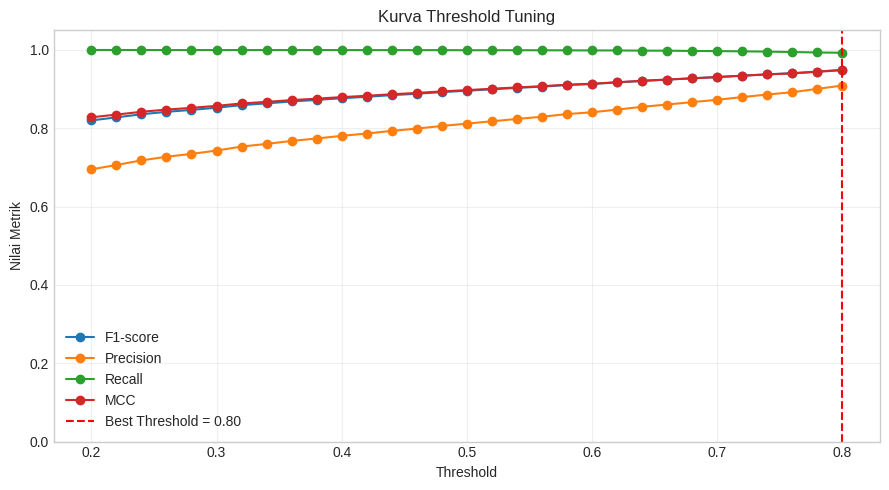
\includegraphics[width=5.51181in,height=3.0375in]{media/media/image16.png}

\phantomsection\label{_Toc228109344}{}Gambar 4. 7 Kurva Treshold Tuning

Berdasarkan Gambar 4.7, perubahan nilai threshold menghasilkan perubahan yang cukup jelas pada~F1,~precision,~recall, dan~MCC. Pola ini menunjukkan bahwa keputusan klasifikasi pada penelitian ini tidak cukup ditetapkan hanya berdasarkan probabilitas model, tetapi perlu disesuaikan melalui pemilihan ambang yang tepat. Oleh karena itu, tahap threshold tuning menjadi bagian penting dalam membentuk konfigurasi model final.

\subsection{Hasil Final Model Evaluation}\label{hasil-final-model-evaluation}

Setelah model final dan threshold terbaik diperoleh, eksperimen dilanjutkan ke evaluasi akhir pada data~test. Hasil evaluasi menunjukkan bahwa model final memiliki performa yang sangat tinggi pada beberapa metrik utama. Evaluasi ini memberikan gambaran mengenai kemampuan generalisasi model terhadap data yang tidak terlibat dalam proses pelatihan dan validasi.

Ringkasan metrik evaluasi akhir pada test set ditunjukkan pada Tabel 4.23.

\phantomsection\label{_Toc228109428}{}Tabel 4. 23 Final Metrics pada Test Set

\begin{longtable}[]{@{}
  >{\raggedright\arraybackslash}p{(\columnwidth - 10\tabcolsep) * \real{0.1931}}
  >{\raggedright\arraybackslash}p{(\columnwidth - 10\tabcolsep) * \real{0.1624}}
  >{\raggedright\arraybackslash}p{(\columnwidth - 10\tabcolsep) * \real{0.1595}}
  >{\raggedright\arraybackslash}p{(\columnwidth - 10\tabcolsep) * \real{0.1661}}
  >{\raggedright\arraybackslash}p{(\columnwidth - 10\tabcolsep) * \real{0.1595}}
  >{\raggedright\arraybackslash}p{(\columnwidth - 10\tabcolsep) * \real{0.1595}}@{}}
\toprule\noalign{}
\begin{minipage}[b]{\linewidth}\raggedright
\textbf{ROC-AUC}
\end{minipage} & \begin{minipage}[b]{\linewidth}\raggedright
\textbf{PR-AUC}
\end{minipage} & \begin{minipage}[b]{\linewidth}\raggedright
\textbf{F1}
\end{minipage} & \begin{minipage}[b]{\linewidth}\raggedright
\textbf{Precision}
\end{minipage} & \begin{minipage}[b]{\linewidth}\raggedright
\textbf{Recall}
\end{minipage} & \begin{minipage}[b]{\linewidth}\raggedright
\textbf{MCC}
\end{minipage} \\
\midrule\noalign{}
\endhead
\bottomrule\noalign{}
\endlastfoot
0,999876 & 0,996046 & 0,952511 & 0,913917 & 0,994507 & 0,951883 \\
\end{longtable}

Berdasarkan Tabel 4.23, model final menghasilkan~ROC-AUC~sebesar 0,999876, PR-AUC sebesar 0,996046, F1 sebesar 0,952511, Precision sebesar 0,913917, Recall~sebesar~0,994507, dan~MCC~sebesar~0,951883. Kombinasi nilai tersebut menunjukkan bahwa model tidak hanya memiliki kemampuan diskriminasi yang sangat tinggi, tetapi juga sangat baik dalam menyeimbangkan ketepatan dan kelengkapan deteksi klaim berisiko.

Untuk melihat hasil klasifikasi secara lebih konkret, confusion matrix model final ditunjukkan pada Gambar 4.8.

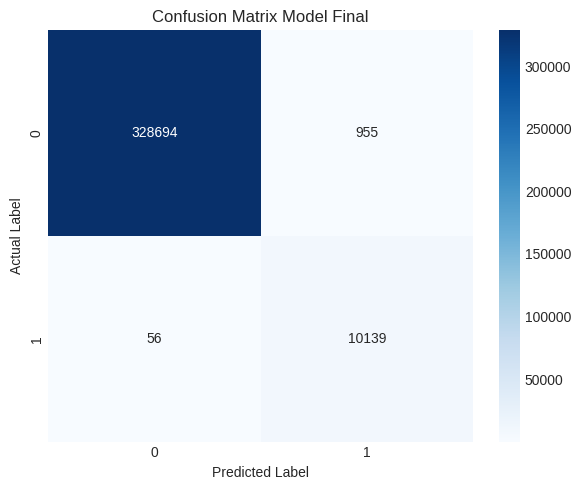
\includegraphics[width=5.51181in,height=4.65in]{media/media/image17.png}

\phantomsection\label{_Toc228109345}{}Gambar 4. 8 Confusion Matrix Model Final

Gambar 4.8 memperlihatkan bahwa model final mampu memisahkan sebagian besar klaim normal dan klaim berisiko secara tepat. Selain itu, untuk menilai kualitas pemeringkatan skor prediksi, kurva ROC dan kurva precision-recall ditunjukkan pada Gambar 4.9 dan Gambar 4.10.

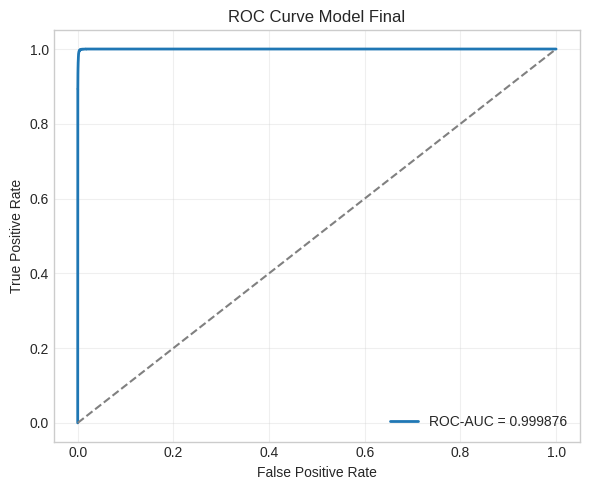
\includegraphics[width=4.93333in,height=4.09733in]{media/media/image18.png}

\phantomsection\label{_Toc228109346}{}Gambar 4. 9 ROC Curve Model Final

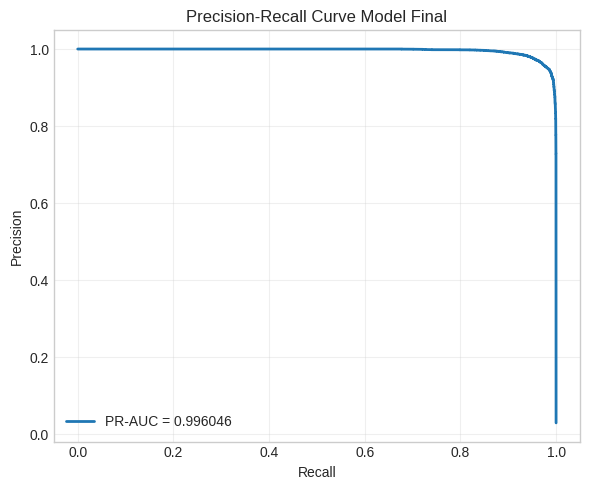
\includegraphics[width=4.87634in,height=4.05in]{media/media/image19.png}

\phantomsection\label{_Toc228109347}{}Gambar 4. 10 Precision-Recall Curve Model Final

Berdasarkan Gambar 4.9 dan Gambar 4.10, model final menunjukkan performa yang sangat baik dalam membedakan kelas dan memeringkat klaim berisiko pada berbagai nilai threshold. Hasil ini konsisten dengan tingginya nilai~ROC-AUC~dan~PR-AUC~yang diperoleh pada Tabel 4.23, sehingga evaluasi akhir menunjukkan bahwa konfigurasi model final memiliki kualitas prediksi yang sangat kuat pada data uji.

\subsection{Hasil Global Interpretability}\label{hasil-global-interpretability}

Setelah evaluasi performa selesai, eksperimen dilanjutkan ke tahap interpretabilitas global. Pada tahap ini, model final dibaca dari sisi fitur-fitur yang paling berpengaruh secara umum terhadap keputusan model. Hasil interpretabilitas global pada penelitian ini diperoleh melalui~feature importance,~SHAP, dan~PDP.

Feature importance~digunakan untuk melihat peringkat fitur dominan yang berkontribusi pada keputusan model final. Hasil ini memberikan gambaran awal mengenai fitur-fitur yang paling sering digunakan model dalam membedakan klaim normal dan klaim berisiko. Ringkasan visual feature importance model final ditunjukkan pada Gambar 4.11.

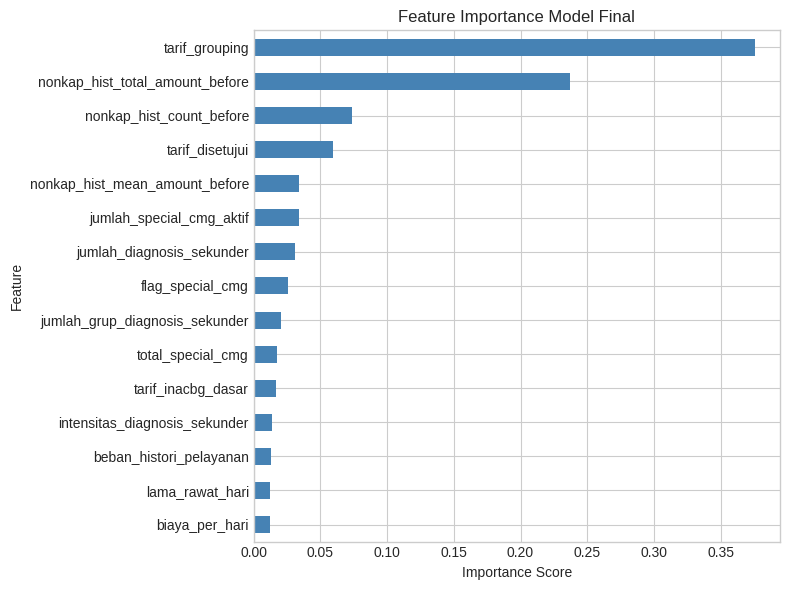
\includegraphics[width=5.51181in,height=4.11597in]{media/media/image20.png}

\phantomsection\label{_Toc228109348}{}Gambar 4. 11 Feature Importance Model Final

Gambar 4.11 menunjukkan peringkat fitur yang paling dominan dalam keputusan model final berdasarkan feature importance. Visualisasi ini memberikan gambaran awal mengenai variabel mana yang paling sering dimanfaatkan model untuk membedakan klaim normal dan klaim berisiko. Fitur-fitur yang berada pada peringkat atas didominasi oleh komponen biaya, histori layanan, dan karakteristik tarif, yang menunjukkan bahwa model sangat peka terhadap pola finansial dan histori utilisasi layanan dalam membaca sinyal risiko.

Selain itu,~SHAP summary plot~digunakan untuk membaca arah dan besar kontribusi fitur terhadap prediksi model. Gambar 4.12 menunjukkan bagaimana setiap fitur memberikan kontribusi yang berbeda terhadap peningkatan atau penurunan skor risiko model.

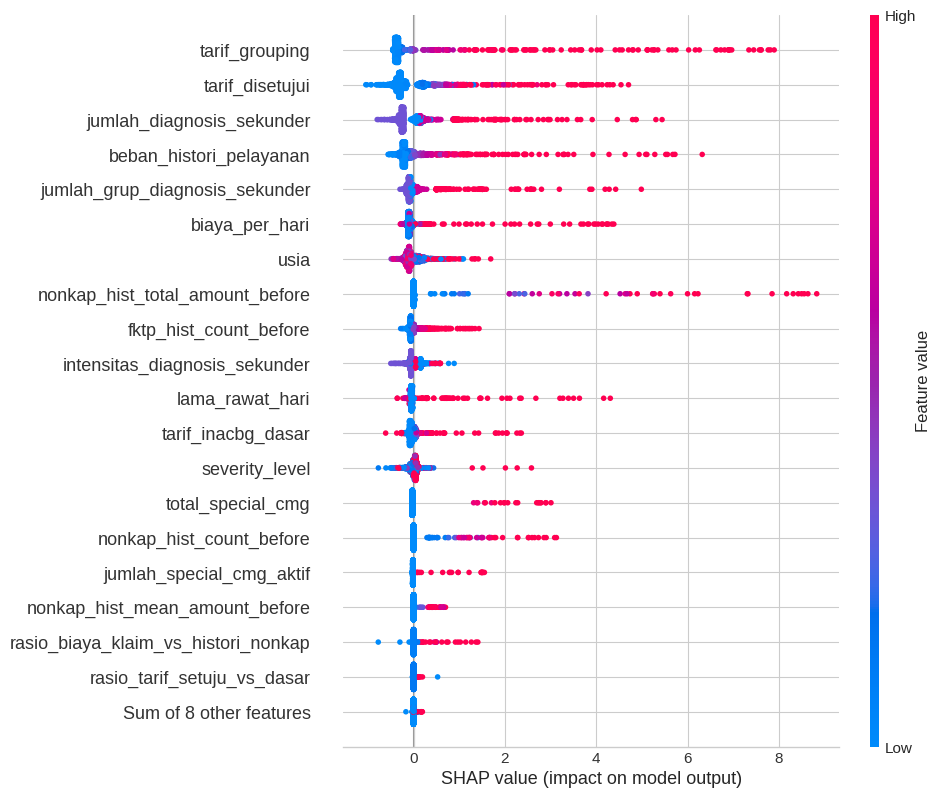
\includegraphics[width=5.51181in,height=4.68125in]{media/media/image21.png}

\phantomsection\label{_Toc228109349}{}Gambar 4. 12 SHAP Summary Plot

Untuk memperjelas pola pengaruh fitur dominan, eksperimen ini juga menghasilkan~PDP~untuk lima fitur teratas, yaitu~tarif\_grouping,~nonkap\_hist\_total\_amount\_before,~nonkap\_hist\_count\_before,~tarif\_disetujui, dan~nonkap\_hist\_mean\_amount\_before. Hasil tersebut ditunjukkan pada Gambar 4.13 sampai Gambar 4.17.

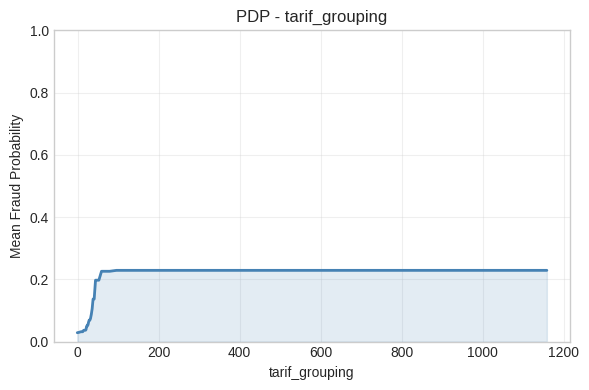
\includegraphics[width=5.51181in,height=3.64861in]{media/media/image22.png}

\phantomsection\label{_Toc228109350}{}Gambar 4. 13 PDP tarif\_groupping

Gambar 4.13 menunjukkan partial dependence plot untuk fitur tarif\_grouping. Kurva ini memperlihatkan bagaimana perubahan nilai tarif\_grouping berasosiasi dengan perubahan rata-rata probabilitas fraud yang diprediksi model. Pola tersebut menunjukkan bahwa tarif\_grouping menjadi salah satu penentu utama dalam pembacaan risiko klaim.

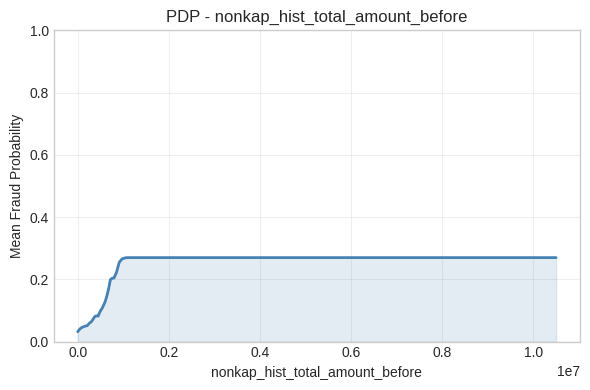
\includegraphics[width=5.51181in,height=3.64375in]{media/media/image23.png}

\phantomsection\label{_Toc228109351}{}Gambar 4. 14 PDP nonkap\_hist\_total\_amount\_before

Gambar 4.14 menunjukkan partial dependence plot untuk fitur nonkap\_hist\_total\_amount\_before. Hasil ini memperlihatkan bahwa histori total biaya nonkapitasi sebelum klaim turut memengaruhi probabilitas fraud, sehingga model tidak hanya membaca klaim saat ini, tetapi juga konteks histori pembiayaan sebelumnya.

Gambar 4.15 menunjukkan partial dependence plot untuk fitur nonkap\_hist\_count\_before. Pola ini menunjukkan bahwa frekuensi layanan nonkapitasi sebelum klaim memiliki kontribusi terhadap perubahan skor risiko, sehingga histori utilisasi layanan menjadi komponen penting dalam analisis.

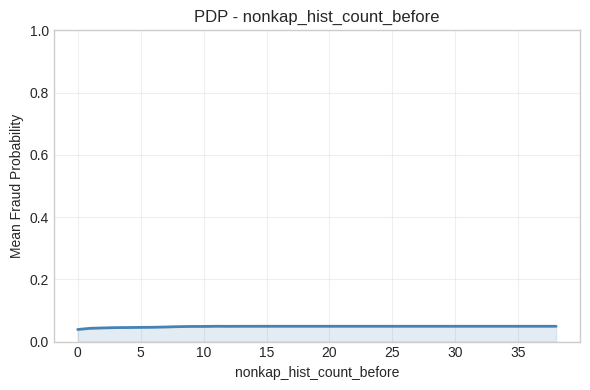
\includegraphics[width=5.51181in,height=3.64375in]{media/media/image24.png}

\phantomsection\label{_Toc228109352}{}Gambar 4. 15 PDP nonkap\_hist\_count\_before

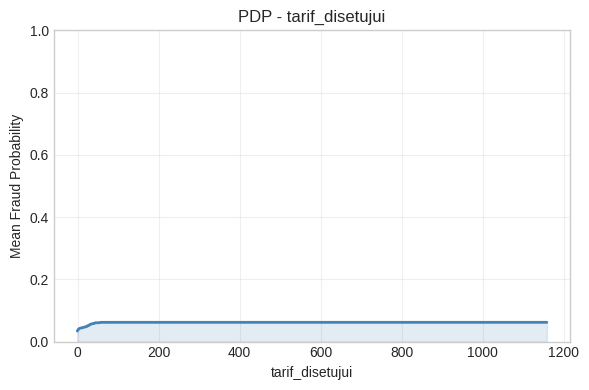
\includegraphics[width=5.51181in,height=3.64861in]{media/media/image25.png}

\phantomsection\label{_Toc228109353}{}Gambar 4. 16 PDP tarif\_disetujui

Gambar 4.16 menunjukkan partial dependence plot untuk fitur tarif\_disetujui. Sebaran pengaruh fitur ini memperlihatkan bahwa nilai biaya klaim yang disetujui memiliki hubungan yang cukup kuat dengan probabilitas fraud, meskipun pengaruhnya tidak selalu linear.

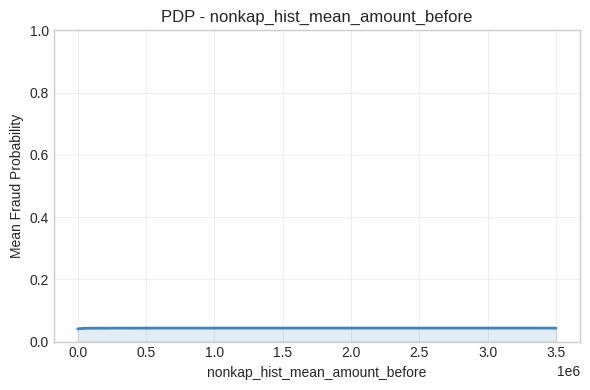
\includegraphics[width=5.51181in,height=3.64375in]{media/media/image26.png}

\phantomsection\label{_Toc228109354}{}Gambar 4. 17 PDP nonkap\_hist\_mean\_amount\_before

Gambar 4.17 menunjukkan partial dependence plot untuk fitur nonkap\_hist\_mean\_amount\_before. Hasil ini menegaskan bahwa rata-rata biaya histori nonkapitasi juga berperan dalam keputusan model, terutama ketika dibaca bersama fitur biaya dan histori lainnya.

Untuk merangkum hasil interpretasi global, Tabel 4.24 disajikan sebagai ringkasan teknik interpretasi, keluaran utama, dan fitur dominan yang muncul pada model final.

\phantomsection\label{_Toc228109429}{}Tabel 4. 24 Ringkasan Interpretasi Global

\begin{longtable}[]{@{}
  >{\raggedright\arraybackslash}p{(\columnwidth - 4\tabcolsep) * \real{0.1783}}
  >{\raggedright\arraybackslash}p{(\columnwidth - 4\tabcolsep) * \real{0.2325}}
  >{\raggedright\arraybackslash}p{(\columnwidth - 4\tabcolsep) * \real{0.5893}}@{}}
\toprule\noalign{}
\begin{minipage}[b]{\linewidth}\raggedright
\textbf{Teknik}
\end{minipage} & \begin{minipage}[b]{\linewidth}\raggedright
\textbf{Output Utama}
\end{minipage} & \begin{minipage}[b]{\linewidth}\raggedright
\textbf{Fitur Dominan}
\end{minipage} \\
\midrule\noalign{}
\endhead
\bottomrule\noalign{}
\endlastfoot
Feature Importance & Peringkat fitur utama & isi dari plot feature importance \\
SHAP & Arah dan besar kontribusi fitur & isi dari summary plot \\
PDP & Pola pengaruh lima fitur utama & tarif\_grouping,~nonkap\_hist\_total\_amount\_before,~nonkap\_hist\_count\_before,~tarif\_disetujui,~nonkap\_hist\_mean\_amount\_before \\
\end{longtable}

Berdasarkan Tabel 4.24, interpretasi global pada penelitian ini menunjukkan bahwa faktor biaya dan histori layanan memiliki kontribusi yang kuat dalam keputusan model final. Kehadiran fitur-fitur seperti~tarif\_grouping,~tarif\_disetujui, dan beberapa variabel histori layanan pada hasil~feature importance,~SHAP, dan~PDP~memperlihatkan bahwa model membaca risiko tidak hanya dari biaya absolut, tetapi juga dari hubungan antara komponen biaya dan pola layanan historis.

\subsection{\texorpdfstring{Hasil \emph{Local Interpretability} dan \emph{Top-Risk Claim Analysis}}{Hasil Local Interpretability dan Top-Risk Claim Analysis}}\label{hasil-local-interpretability-dan-top-risk-claim-analysis}

Setelah interpretasi global dilakukan, eksperimen dilanjutkan ke tahap interpretasi lokal pada klaim-klaim dengan probabilitas fraud tertinggi. Tahap ini bertujuan untuk menjelaskan alasan prediksi model pada level klaim individual. Dengan pendekatan ini, analisis tidak berhenti pada pola umum populasi, tetapi masuk ke level observasi individual yang paling relevan untuk ditelaah lebih lanjut.

Hasil eksperimen menunjukkan tiga klaim dengan probabilitas fraud tertinggi, yaitu 10241124V003022,~452460624V011711, dan~397950224V011829. Ketiga klaim tersebut memiliki probabilitas prediksi yang sangat tinggi dan kemudian dianalisis lebih lanjut menggunakan~LIME~untuk melihat fitur-fitur yang paling mendorong keputusan model. Ringkasan klaim berisiko tertinggi ditunjukkan pada Tabel 4.25.

\phantomsection\label{_Toc228109430}{}Tabel 4. 25 Top-Risk Claims

\begin{longtable}[]{@{}
  >{\raggedright\arraybackslash}p{(\columnwidth - 6\tabcolsep) * \real{0.0980}}
  >{\raggedright\arraybackslash}p{(\columnwidth - 6\tabcolsep) * \real{0.2763}}
  >{\raggedright\arraybackslash}p{(\columnwidth - 6\tabcolsep) * \real{0.2059}}
  >{\raggedright\arraybackslash}p{(\columnwidth - 6\tabcolsep) * \real{0.4198}}@{}}
\toprule\noalign{}
\begin{minipage}[b]{\linewidth}\raggedright
\textbf{Rank}
\end{minipage} & \begin{minipage}[b]{\linewidth}\raggedright
\textbf{ID Klaim}
\end{minipage} & \begin{minipage}[b]{\linewidth}\raggedright
\textbf{Fraud Probability}
\end{minipage} & \begin{minipage}[b]{\linewidth}\raggedright
\textbf{Faktor Utama}
\end{minipage} \\
\midrule\noalign{}
\endhead
\bottomrule\noalign{}
\endlastfoot
1 & 10241124V003022 & 1,0000 & histori nonkapitasi, tarif grouping, rasio tarif, tarif disetujui \\
2 & 452460624V011711 & 1,0000 & histori nonkapitasi, total special CMG, tarif grouping, special CMG \\
3 & 397950224V011829 & 1,0000 & tarif grouping, lama rawat, diagnosis sekunder, tarif disetujui \\
\end{longtable}

Berdasarkan Tabel 4.25, ketiga klaim teratas memiliki probabilitas fraud yang sangat tinggi dan didorong oleh kombinasi fitur yang berkaitan dengan komponen biaya, histori nonkapitasi, tarif grouping, dan beberapa indikator klinis tertentu. Hal ini menunjukkan bahwa keputusan model pada level lokal tetap konsisten dengan pola yang sudah terlihat pada interpretasi global.

Untuk memperjelas alasan prediksi pada ketiga klaim tersebut, hasil local explanation ditunjukkan pada Gambar 4.18 sampai Gambar 4.20.

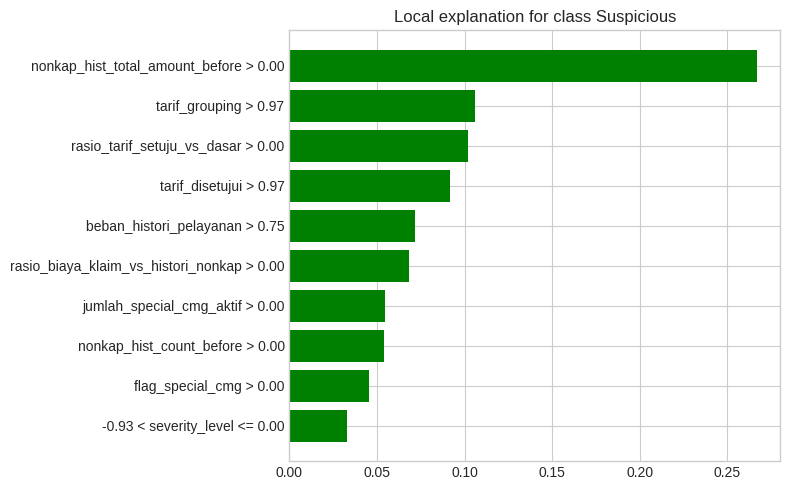
\includegraphics[width=5.51181in,height=3.41875in]{media/media/image27.png}

\phantomsection\label{_Toc228109355}{}Gambar 4. 18 Hasil LIME pada klaim 10241124V003022

Gambar 4.18 menunjukkan local explanation untuk klaim dengan probabilitas fraud tertinggi pertama. Hasil LIME memperlihatkan bahwa prediksi model terutama didorong oleh kombinasi histori nonkapitasi, tarif grouping, rasio tarif, dan tarif disetujui. Pola ini menunjukkan bahwa klaim tersebut dinilai berisiko karena memiliki karakteristik finansial dan histori layanan yang menyimpang dibandingkan populasi normal.

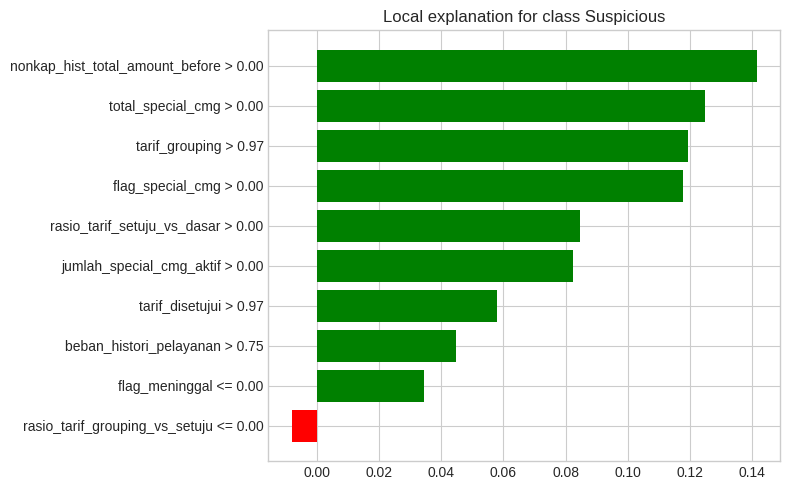
\includegraphics[width=5.51181in,height=3.41875in]{media/media/image28.png}

\phantomsection\label{_Toc228109356}{}Gambar 4. 19 Hasil LIME untuk pada 452460624V011711

Gambar 4.19 menunjukkan local explanation untuk klaim dengan probabilitas fraud tertinggi kedua. Pada klaim ini, faktor dominan yang mendorong skor risiko adalah histori nonkapitasi, total special CMG, tarif grouping, dan special CMG. Hal ini menunjukkan bahwa selain komponen biaya utama, tambahan biaya berbasis kompleksitas layanan juga berperan penting dalam keputusan model.

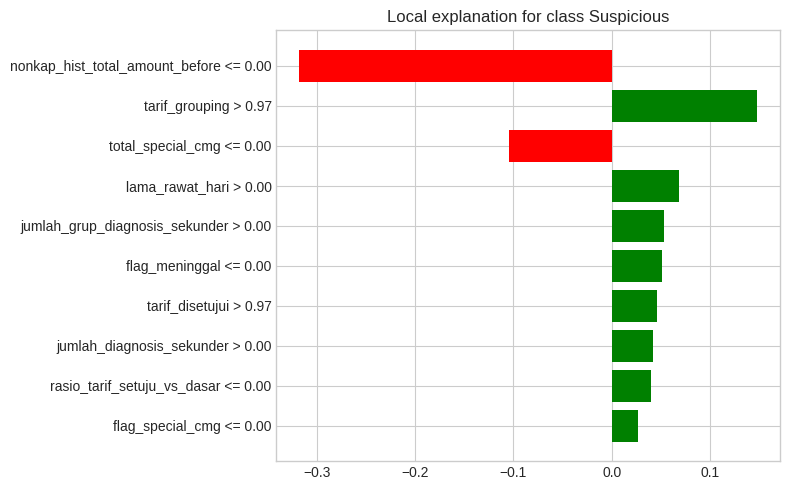
\includegraphics[width=5.51181in,height=3.41875in]{media/media/image29.png}

\phantomsection\label{_Toc228109357}{}Gambar 4. 20 Hasil LIME pada klaim 397950224V011829

Gambar 4.20 menunjukkan local explanation untuk klaim dengan probabilitas fraud tertinggi ketiga. Faktor yang paling berpengaruh pada klaim ini meliputi tarif grouping, lama rawat, diagnosis sekunder, dan tarif disetujui. Pola tersebut memperlihatkan bahwa model juga mempertimbangkan kombinasi aspek klinis dan finansial secara bersama dalam membaca risiko pada level klaim individual.

Berdasarkan Gambar 4.18 sampai Gambar 4.20, faktor pendorong utama pada ketiga klaim risiko tertinggi tidak sepenuhnya identik, tetapi memiliki pola umum yang serupa, yaitu dominasi komponen biaya dan histori layanan dalam mendorong skor risiko ke arah yang lebih tinggi. Dengan demikian, local interpretability pada penelitian ini menunjukkan bahwa model final tidak hanya kuat pada level populasi, tetapi juga dapat dibaca pada level klaim individual.

\subsection{Hasil Export Artifacts}\label{hasil-export-artifacts}

Tahap akhir dari eksperimen adalah penyimpanan artefak hasil. Artefak ini diekspor untuk memastikan bahwa keluaran utama dari pipeline dapat digunakan kembali untuk pelaporan, dokumentasi, dan verifikasi hasil eksperimen. Dengan adanya artefak tersebut, hasil eksperimen tidak hanya tersaji di lingkungan notebook, tetapi juga tersedia dalam bentuk keluaran yang terstruktur.

Artefak yang disimpan pada penelitian ini mencakup informasi model pemenang, hasil analisis threshold, daftar klaim berisiko tinggi, metrik evaluasi akhir, dan laporan interpretabilitas. Masing-masing artefak memiliki fungsi yang berbeda dalam mendukung pembacaan hasil pada Bab 4. Ringkasan artefak hasil yang diekspor ditunjukkan pada Tabel 4.26.

\phantomsection\label{_Toc228109431}{}Tabel 4. 26 Artefak Hasil yang Diekspor

\begin{longtable}[]{@{}
  >{\raggedright\arraybackslash}p{(\columnwidth - 4\tabcolsep) * \real{0.2542}}
  >{\raggedright\arraybackslash}p{(\columnwidth - 4\tabcolsep) * \real{0.4244}}
  >{\raggedright\arraybackslash}p{(\columnwidth - 4\tabcolsep) * \real{0.3214}}@{}}
\toprule\noalign{}
\begin{minipage}[b]{\linewidth}\raggedright
\textbf{Nama Artefak}
\end{minipage} & \begin{minipage}[b]{\linewidth}\raggedright
\textbf{Isi}
\end{minipage} & \begin{minipage}[b]{\linewidth}\raggedright
\textbf{Kegunaan}
\end{minipage} \\
\midrule\noalign{}
\endhead
\bottomrule\noalign{}
\endlastfoot
winner info & informasi winner branch, winner model, fitur, threshold & dokumentasi konfigurasi model final \\
threshold analysis & performa model pada berbagai threshold & dasar pemilihan threshold \\
top-risk claims & daftar klaim dengan probabilitas tertinggi & dasar analisis lokal \\
final metrics & metrik akhir model pada test set & pelaporan performa \\
laporan interpretability & keluaran SHAP, PDP, LIME, feature importance & menjelaskan hasil prediksi \\
\end{longtable}

Berdasarkan Tabel 4.26, artefak hasil pada penelitian ini tidak hanya berfungsi sebagai dokumentasi teknis, tetapi juga sebagai penghubung antara pelaksanaan eksperimen dan penulisan hasil.~winner info~dan~threshold analysis~mendokumentasikan konfigurasi model final,~top-risk claims~mendukung analisis lokal,~final metrics~mendukung pelaporan performa model, sedangkan laporan interpretabilitas membantu menjelaskan dasar keputusan model. Dengan adanya artefak-artefak ini, hasil eksperimen menjadi lebih mudah diverifikasi dan digunakan kembali pada tahap analisis.

\section{ANALISIS HASIL EKSPERIMEN}\label{analisis-hasil-eksperimen}

Subbab ini menganalisis hasil eksperimen yang telah disajikan pada Subbab 4.6. Analisis dilakukan secara paralel terhadap tahapan eksperimen, sehingga setiap keluaran utama tidak hanya ditampilkan sebagai hasil numerik atau visual, tetapi juga dijelaskan maknanya dalam konteks deteksi potensi fraud atau upcoding pada klaim JKN/BPJS. Dengan pendekatan tersebut, pembahasan pada subbab ini tidak mengulang hasil secara mentah, melainkan menafsirkan hasil tersebut dalam kaitannya dengan kualitas data, konfigurasi eksperimen, performa model, dan tujuan penelitian.

Analisis hasil eksperimen pada penelitian ini tidak hanya berfokus pada seberapa tinggi performa model, tetapi juga pada bagaimana model tersebut dibentuk, mengapa konfigurasi tertentu memberikan hasil yang lebih baik, dan apakah keluaran model dapat dijelaskan secara analitis. Oleh karena itu, subbab ini berfungsi untuk menghubungkan hasil eksperimen dengan logika metodologis penelitian serta menjelaskan kontribusinya terhadap tujuan penelitian secara utuh.

\subsection{Analisis Integrasi Claim-Centric dan Karakteristik Dataset}\label{analisis-integrasi-claim-centric-dan-karakteristik-dataset}

Hasil integrasi claim-centric pada Tabel 4.16 memperlihatkan bahwa satu klaim tetap dapat dipertahankan sebagai unit observasi utama meskipun data berasal dari beberapa sumber yang berbeda. Pendekatan ini penting karena model tidak hanya membaca klaim sebagai catatan biaya tunggal, tetapi sebagai entitas yang diperkaya oleh atribut peserta, diagnosis sekunder, dan histori layanan. Dengan demikian, struktur data akhir yang terbentuk lebih representatif untuk mendukung analisis risiko pada level transaksi klaim.

Integrasi multi-tabel juga memperkuat konteks analisis karena setiap sumber data memberikan kontribusi yang berbeda. Informasi dari kepesertaan memberikan konteks administratif dan demografis peserta, diagnosissekunder menambah kedalaman klinis, sedangkan fktpkapitasi dan nonkapitasi memberikan dimensi historis yang tidak tersedia pada klaim utama. Hasil integrasi seperti yang dirangkum pada Tabel 4.16 menunjukkan bahwa model pada penelitian ini dibangun di atas data yang lebih kaya daripada jika hanya bergantung pada tabel klaim mentah.

Karakteristik dataset yang ditunjukkan pada Tabel 4.10 dan Tabel 4.12 juga memperlihatkan bahwa data yang digunakan memiliki keragaman yang tinggi, baik dari sisi ukuran, tipe variabel, maupun dimensi informasinya. Variasi ini menjadi kekuatan sekaligus tantangan. Di satu sisi, keragaman tersebut memberikan sinyal yang lebih kaya untuk deteksi fraud. Di sisi lain, keragaman itu juga menuntut proses integrasi, standardisasi, dan seleksi fitur yang lebih ketat agar model tidak dibebani oleh variabel yang redundan atau kurang relevan.

Secara analitis, pendekatan claim-centric pada penelitian ini dapat dinilai lebih sesuai dengan tujuan deteksi fraud/upcoding karena fokusnya langsung berada pada klaim yang akan dievaluasi. Dengan struktur tersebut, eksperimen tidak hanya mampu membangun dataset pada level klaim, tetapi juga membentuk dasar yang lebih kuat untuk seluruh tahap pemodelan berikutnya.

\subsection{Analisis Pembentukan Pseudo-Label}\label{analisis-pembentukan-pseudo-label}

Dalam konteks penelitian ini, pseudo-label memiliki makna yang sangat penting karena berfungsi sebagai pengganti target pembelajaran pada kondisi ketika label fraud aktual tidak tersedia pada level klaim. Hasil pada Tabel 4.18 menunjukkan bahwa pseudo-label dibentuk melalui Isolation Forest dengan variasi contamination rate, sehingga eksperimen memiliki dasar yang lebih terukur dalam menentukan proporsi anomali yang akan digunakan sebagai target awal.

Nilai fraud ratio sekitar 3\% yang dihasilkan pada konfigurasi final menunjukkan bahwa klaim yang ditandai sebagai anomali memang hanya merupakan bagian kecil dari populasi. Secara analitis, hasil ini sesuai dengan karakter umum masalah fraud detection, di mana kejadian berisiko cenderung jarang dibandingkan dengan klaim normal. Artinya, pseudo-label yang terbentuk masih realistis dalam merepresentasikan sifat kasus yang hendak dideteksi, yaitu risiko fraud sebagai kelompok minoritas.

Perbandingan profil median antara klaim normal dan suspicious pada Gambar 4.6 memperlihatkan bahwa kelompok klaim anomali memiliki karakteristik yang berbeda secara cukup jelas dibandingkan Meioritas klaim. Klaim suspicious cenderung memiliki nilai median yang lebih tinggi pada beberapa indikator biaya dan layanan, sehingga pseudo-label yang terbentuk tidak bersifat acak. Pola ini menunjukkan bahwa Isolation Forest memang menangkap kelompok klaim yang memiliki struktur numerik berbeda dari populasi normal.

Dengan demikian, pseudo-label pada penelitian ini dapat dipahami bukan sebagai label fraud final, tetapi sebagai target awal yang cukup informatif untuk mendorong tahap supervised learning. Keberhasilan tahap ini penting karena seluruh proses benchmarking berikutnya bergantung pada kualitas target yang dibentuk pada tahap pseudo-labeling.

\subsection{Analisis Split, Preprocessing, dan Branch-Based Feature Selection}\label{analisis-split-preprocessing-dan-branch-based-feature-selection}

Hasil split dataset pada Tabel 4.19 menunjukkan bahwa distribusi label tetap konsisten pada subset train, validation, dan test, dengan rasio pseudo-label positif yang relatif sama pada ketiganya. Konsistensi ini penting karena menjaga agar pelatihan, validasi, dan evaluasi dilakukan pada distribusi kelas yang sebanding. Secara analitis, hasil ini menunjukkan bahwa proses pembagian data berjalan dengan baik dan tidak menimbulkan pergeseran distribusi yang dapat mengganggu pembacaan performa model.

Aspek berikutnya yang penting adalah kontrol terhadap data leakage. Pemisahan data lebih dahulu sebelum preprocessing dan pemodelan memastikan bahwa informasi dari data uji tidak bocor ke tahap pelatihan. Dalam penelitian ini, kontrol seperti itu menjadi krusial karena dataset sangat besar dan kaya fitur, sehingga tanpa pengendalian yang tepat, model berisiko memberikan performa yang tampak tinggi tetapi tidak benar-benar merepresentasikan kemampuan generalisasi.

Hasil branch-based feature selection pada Tabel 4.20 menunjukkan bahwa setiap branch menghasilkan jumlah dan karakter fitur yang berbeda. Dari hasil eksperimen, branch vif terbukti memberikan kombinasi paling efektif ketika dipadukan dengan model terbaik pada tahap benchmarking. Secara analitis, hasil ini menunjukkan bahwa pengurangan multikolinearitas memberikan manfaat yang nyata terhadap performa model. Dengan menekan redundansi hubungan linear antarfitur, branch vif memungkinkan model bekerja pada himpunan variabel yang lebih stabil dan lebih informatif.

Dengan demikian, hasil split, preprocessing, dan feature selection tidak boleh dipandang sebagai tahap teknis semata. Ketiganya justru berperan langsung dalam membentuk kualitas masukan model. Keberhasilan branch vif menunjukkan bahwa performa terbaik pada penelitian ini tidak hanya bergantung pada algoritma, tetapi juga pada kualitas struktur fitur yang digunakan.

\subsection{Analisis Benchmarking, Winner Selection, dan Threshold Tuning}\label{analisis-benchmarking-winner-selection-dan-threshold-tuning}

Hasil benchmarking pada Tabel 4.21 menunjukkan bahwa model final pada penelitian ini dipilih secara empiris berdasarkan performa aktual pada berbagai kombinasi branch dan algoritma. Hasil ini penting karena membuktikan bahwa konfigurasi terbaik tidak diasumsikan sejak awal, tetapi diperoleh melalui proses pembandingan yang sistematis. Dengan demikian, pemilihan model final benar-benar merupakan keluaran dari eksperimen, bukan keputusan yang ditetapkan secara apriori.

Dari seluruh kombinasi yang diuji, XGBoost pada branch vif menempati posisi terbaik dan kemudian ditetapkan sebagai winner, sebagaimana dirangkum pada Tabel 4.22. Hasil ini menunjukkan bahwa kombinasi antara model boosting dan himpunan fitur yang telah dikurangi multikolinearitasnya memberikan performa paling kuat pada data validasi. Keunggulan tersebut juga menegaskan bahwa struktur fitur memegang peran yang sama pentingnya dengan pemilihan algoritma.

Nilai threshold terbaik sebesar 0,80 memiliki arti penting secara analitis. Threshold ini menunjukkan bahwa klasifikasi akhir tidak dilakukan pada ambang probabilitas standar secara otomatis, tetapi melalui proses penyesuaian agar keseimbangan antara precision, recall, F1, dan MCC dapat dioptimalkan. Hubungan antar metrik terhadap perubahan threshold dapat dilihat pada Gambar 4.7, yang menunjukkan bahwa perubahan ambang klasifikasi menghasilkan perubahan performa yang cukup nyata.

Secara lebih spesifik, threshold yang lebih tinggi cenderung mendorong precision menjadi lebih baik, tetapi juga dapat menurunkan recall jika terlalu ketat. Sebaliknya, threshold yang lebih rendah cenderung memperbesar cakupan deteksi namun berpotensi meningkatkan false positive. Oleh karena itu, hasil pada Gambar 4.7 memperlihatkan bahwa threshold 0,80 dipilih karena memberikan titik keseimbangan yang paling sesuai dengan tujuan deteksi risiko pada penelitian ini.

\subsection{Analisis Kinerja Model Final}\label{analisis-kinerja-model-final}

Hasil evaluasi model final pada Tabel 4.23 menunjukkan bahwa model memiliki performa yang sangat tinggi terhadap target pseudo-label yang dibentuk pada tahap sebelumnya. Nilai ROC-AUC sebesar 0,999876 dan PR-AUC sebesar 0,996046 menunjukkan bahwa model sangat baik dalam membedakan klaim normal dan klaim berisiko serta dalam memeringkat probabilitas risiko pada kondisi data yang tidak seimbang.

Nilai F1-score sebesar 0,952511 menunjukkan keseimbangan yang sangat baik antara precision dan recall. Precision sebesar 0,913917 menunjukkan bahwa sebagian besar klaim yang ditandai berisiko memang relevan untuk diperhatikan lebih lanjut, sedangkan recall sebesar 0,994507 menunjukkan bahwa hampir seluruh klaim berisiko menurut pseudo-label berhasil ditangkap oleh model. Nilai MCC sebesar 0,951883 juga memperkuat bahwa performa model tetap tinggi ketika dievaluasi dengan metrik yang lebih seimbang pada distribusi kelas yang tidak merata.

Namun demikian, hasil ini perlu dibaca secara proporsional. Performa yang sangat tinggi pada penelitian ini menunjukkan kemampuan model dalam mempelajari dan memprediksi sinyal risiko yang dibentuk melalui pseudo-labeling, bukan secara langsung membuktikan kemampuan model dalam mengidentifikasi fraud aktual hasil audit resmi. Oleh karena itu, kekuatan utama model pada tahap ini adalah sebagai mekanisme penyaringan awal yang terukur, konsisten, dan siap digunakan untuk mendukung prioritisasi pemeriksaan klaim.

Dari sisi generalisasi, keberhasilan model pada data test tetap menunjukkan bahwa pipeline yang dibangun bekerja dengan baik pada data yang tidak terlibat dalam pelatihan dan validasi. Hasil pada Gambar 4.8, Gambar 4.9, dan Gambar 4.10 memperlihatkan bahwa model memiliki pemisahan kelas yang sangat baik pada confusion matrix serta kualitas pemeringkatan yang kuat pada kurva ROC dan precision-recall. Dengan demikian, model final dapat diposisikan sebagai alat bantu analitis yang kuat untuk mendukung proses verifikasi, dengan tetap menempatkan pembuktian fraud pada audit dan pemeriksaan lanjutan.

\subsection{Analisis Interpretabilitas Global dan Lokal}\label{analisis-interpretabilitas-global-dan-lokal}

Hasil interpretabilitas global pada Gambar 4.11, Gambar 4.12, dan Gambar 4.13 sampai Gambar 4.17 menunjukkan bahwa model final dipengaruhi secara kuat oleh fitur-fitur yang berkaitan dengan biaya, histori layanan nonkapitasi, dan komponen tarif. Temuan ini penting karena menunjukkan bahwa model tidak sekadar belajar dari satu indikator biaya tunggal, tetapi dari hubungan beberapa indikator finansial dan historis yang secara bersama-sama membentuk sinyal risiko.

Feature importance pada Gambar 4.11 memberikan gambaran awal mengenai fitur yang paling dominan pada keputusan model. Pembacaan ini menjadi lebih bermakna ketika dikombinasikan dengan SHAP pada Gambar 4.12, karena SHAP memperlihatkan arah dan besar kontribusi fitur terhadap prediksi. Dari kedua visual tersebut dapat dilihat bahwa beberapa fitur biaya, tarif grouping, serta histori layanan memiliki pengaruh yang kuat terhadap peningkatan skor risiko model.

PDP pada Gambar 4.13 sampai Gambar 4.17 memperdalam interpretasi tersebut dengan menunjukkan bahwa pengaruh fitur tidak selalu bersifat linier. Fitur seperti tarif\_grouping, nonkap\_hist\_total\_amount\_before, nonkap\_hist\_count\_before, tarif\_disetujui, dan nonkap\_hist\_mean\_amount\_before tidak hanya penting, tetapi juga memiliki pola pengaruh tertentu terhadap probabilitas fraud. Hal ini menunjukkan bahwa model menangkap hubungan yang lebih kompleks daripada sekadar hubungan sederhana antara biaya tinggi dan risiko tinggi.

Dari sisi interpretabilitas lokal, hasil pada Gambar 4.18 sampai Gambar 4.20 dan Tabel 4.25 menunjukkan bahwa tiga klaim dengan probabilitas fraud tertinggi memiliki pola risiko yang tetap konsisten dengan temuan global, yaitu dominasi faktor biaya, histori nonkapitasi, tarif grouping, serta beberapa indikator klinis tambahan. Namun demikian, masing-masing klaim tetap memiliki kombinasi faktor pendorong yang tidak sepenuhnya identik. Hal ini menunjukkan bahwa model final pada penelitian ini mampu menilai risiko secara individual, bukan hanya berdasarkan pola umum populasi.

Secara analitis, hubungan antara biaya, histori layanan nonkapitasi, tarif grouping, dan sinyal risiko menjadi salah satu temuan penting dalam penelitian ini. Temuan ini menunjukkan bahwa klaim berisiko tidak terbaca hanya dari tingginya biaya, tetapi dari kombinasi pola biaya, struktur tarif, dan riwayat layanan yang membentuk konteks ketidakwajaran. Bagi auditor atau verifikator, hasil interpretabilitas ini bernilai penting karena menyediakan alasan analitis di balik skor risiko, sehingga keluaran model dapat dibaca sebagai dasar prioritas pemeriksaan, bukan sekadar label prediksi yang berdiri sendiri.

\subsection{Keterkaitan Hasil Eksperimen dengan Tujuan Penelitian}\label{keterkaitan-hasil-eksperimen-dengan-tujuan-penelitian}

Secara keseluruhan, hasil eksperimen menunjukkan bahwa sistem yang dibangun pada penelitian ini berhasil mendeteksi potensi fraud atau upcoding pada level klaim. Keberhasilan tersebut terlihat dari terbentuknya pseudo-label yang informatif, pemilihan model final melalui benchmarking yang terukur, performa evaluasi yang sangat tinggi pada data uji, serta tersedianya interpretasi global dan lokal terhadap hasil prediksi. Dengan demikian, tujuan utama penelitian, yaitu membangun mekanisme analitis untuk menandai klaim berisiko, dapat dinyatakan tercapai.

Hasil eksperimen ini juga menunjukkan bahwa pipeline yang digunakan mampu bekerja secara konsisten dengan rancangan sistem yang telah dibangun sebelumnya. Alur mulai dari integrasi claim-centric, pseudo-labeling, branch-based feature selection, benchmarking multi-model, threshold tuning, hingga interpretabilitas terbukti dapat dijalankan secara utuh dan menghasilkan keluaran yang saling terhubung. Dengan kata lain, hasil eksperimen tidak berdiri sendiri, tetapi merupakan implementasi operasional dari kerangka sistem yang dirancang dalam penelitian ini.

Di samping itu, hasil penelitian menunjukkan bahwa sistem yang dibangun tidak hanya berfungsi untuk melakukan prediksi, tetapi juga mampu menjelaskan alasan di balik prediksi tersebut. Kehadiran feature importance, SHAP, PDP, dan LIME memperlihatkan bahwa keluaran model dapat dibaca dari dua tingkat sekaligus, yaitu tingkat populasi dan tingkat klaim individual. Hal ini penting karena pada domain klaim kesehatan, kemampuan menjelaskan hasil prediksi merupakan bagian yang sangat menentukan nilai praktis suatu sistem analitis.

Dengan demikian, jawaban terhadap tujuan penelitian dapat ditegaskan secara eksplisit sebagai berikut. Tujuan untuk membangun data analisis berbasis klaim telah tercapai melalui integrasi claim-centric. Tujuan untuk membentuk indikasi risiko awal telah tercapai melalui pseudo-labeling dengan Isolation Forest. Tujuan untuk menerapkan dan membandingkan beberapa model machine learning telah tercapai melalui benchmarking multi-model. Tujuan untuk menentukan konfigurasi keputusan terbaik telah tercapai melalui winner selection dan threshold tuning. Tujuan untuk menjelaskan hasil deteksi juga telah tercapai melalui interpretabilitas global dan lokal. Oleh karena itu, penelitian ini tidak hanya menghasilkan model klasifikasi, tetapi juga menghasilkan mekanisme analitis yang terstruktur, terukur, dan dapat dijelaskan untuk mendukung prioritisasi verifikasi klaim berisiko tinggi.

\emph{(Halaman ini sengaja dikosongkan)}

%============================================================
% BAB 5 — hasil konversi awal dari DOCX lama
%============================================================
\chapter{PENUTUP}

Bab ini menyajikan kesimpulan dan saran berdasarkan hasil perancangan sistem, pelaksanaan eksperimen, serta analisis kinerja model deteksi potensi fraud/upcoding pada klaim JKN/BPJS dalam sistem INA-CBG. Kesimpulan disusun untuk menjawab permasalahan dan tujuan penelitian, sedangkan saran diberikan sebagai arahan pengembangan agar pendekatan yang dibangun dapat diuji dan disempurnakan pada penelitian berikutnya.

\section{KESIMPULAN}\label{kesimpulan}

Berdasarkan hasil penelitian yang telah dilakukan, diperoleh beberapa kesimpulan sebagai berikut.

\begin{enumerate}
\def\labelenumi{\arabic{enumi}.}
\item
  Deteksi potensi fraud/upcoding pada klaim JKN/BPJS dalam sistem INA-CBG merupakan permasalahan yang penting karena nilai klaim dipengaruhi oleh diagnosis, prosedur, tingkat keparahan, jenis layanan, dan komponen tarif. Dalam kondisi volume klaim yang besar, proses verifikasi membutuhkan dukungan analitik untuk membantu memprioritaskan klaim berisiko.
\item
  Penelitian ini mengajukan pendekatan machine learning berbasis claim-centric, yaitu menjadikan satu klaim sebagai unit analisis utama dan memperkaya klaim dengan data kepesertaan, diagnosis sekunder, serta histori layanan. Pendekatan ini dirancang agar pembacaan risiko tidak hanya bertumpu pada satu komponen biaya, tetapi pada konteks administratif, klinis, dan historis yang melekat pada klaim.
\item
  Orisinalitas penelitian ini terletak pada penyusunan pipeline deteksi potensi fraud/upcoding yang utuh pada konteks klaim JKN/BPJS, meliputi claim-centric data preparation, pseudo-labeling dengan Isolation Forest, branch-based feature selection, supervised benchmarking multi-model, threshold tuning, serta interpretabilitas global dan lokal.
\item
  Hasil eksperimen menunjukkan bahwa ketika label fraud aktual tidak tersedia, pseudo-label dapat dibentuk secara terukur dan digunakan sebagai target awal untuk supervised learning. Dari proses benchmarking, kombinasi XGBoost pada branch VIF dengan threshold 0,80 memberikan performa terbaik pada data uji terhadap target pseudo-label, dengan ROC-AUC 0,999876, PR-AUC 0,996046, F1-score 0,952511, precision 0,913917, recall 0,994507, dan MCC 0,951883.
\item
  Hasil interpretabilitas menunjukkan bahwa faktor biaya, tarif grouping, histori layanan nonkapitasi, special CMG, dan rasio tarif merupakan pendorong penting skor risiko. Temuan ini menunjukkan bahwa model tidak hanya menghasilkan prediksi, tetapi juga menyediakan dasar analitis yang dapat membantu pembacaan klaim berisiko.
\item
  Secara keseluruhan, sistem yang dibangun layak diposisikan sebagai alat bantu prioritisasi pemeriksaan klaim berisiko tinggi. Meskipun demikian, hasil penelitian tetap harus dipahami sebagai deteksi indikasi risiko berbasis pseudo-label, bukan sebagai pembuktian fraud aktual secara hukum atau audit resmi.
\end{enumerate}

\section{SARAN}\label{saran}

Berdasarkan hasil dan keterbatasan penelitian, beberapa saran untuk pengembangan penelitian berikutnya adalah sebagai berikut.

\begin{enumerate}
\def\labelenumi{\arabic{enumi}.}
\item
  Penelitian berikutnya disarankan melakukan validasi menggunakan label hasil audit atau verifikasi resmi. Pada penelitian ini, target pembelajaran dibentuk melalui pseudo-label karena label fraud aktual pada level klaim tidak tersedia. Oleh karena itu, pengujian terhadap label audit resmi diperlukan untuk mengetahui kesesuaian skor risiko model dengan keputusan ahli, serta untuk membedakan lebih jelas antara klaim yang benar-benar bermasalah, klaim yang hanya anomali secara data, dan klaim yang valid tetapi memiliki karakteristik tidak umum.
\item
  Cakupan data dapat diperluas pada periode, wilayah, dan jenis fasilitas kesehatan yang lebih beragam. Pengujian lintas periode diperlukan untuk melihat kestabilan pola risiko dari waktu ke waktu, sedangkan pengujian lintas wilayah dan fasilitas kesehatan diperlukan untuk menilai apakah model tetap konsisten pada variasi karakteristik rumah sakit, komposisi pasien, pola layanan, dan struktur klaim yang berbeda.
\item
  Penelitian lanjutan dapat menambahkan data klinis dan administratif yang lebih lengkap, seperti ringkasan rekam medis, hasil verifikasi klaim, catatan dispute, catatan revisi kode, serta informasi pendukung dari proses koding. Pengayaan data tersebut dapat membantu model membedakan klaim yang memang memiliki kebutuhan klinis kompleks dari klaim yang memiliki indikasi risiko upcoding, sehingga interpretasi hasil deteksi menjadi lebih kuat.
\item
  Sistem perlu diuji dalam skenario operasional bersama auditor atau verifikator klaim. Pengujian tersebut penting untuk menilai apakah daftar klaim berisiko tinggi, skor risiko, dan penjelasan faktor prediksi benar-benar membantu proses prioritisasi pemeriksaan. Evaluasi operasional juga dapat mengukur aspek kegunaan sistem, seperti kemudahan membaca hasil, waktu yang dibutuhkan untuk meninjau klaim, dan kesesuaian keluaran model dengan kebutuhan kerja verifikasi.
\item
  Pengembangan selanjutnya dapat diarahkan pada dashboard monitoring yang menampilkan skor risiko, peringkat klaim berisiko tinggi, faktor pendorong prediksi, serta ringkasan interpretabilitas global dan lokal. Dashboard tersebut sebaiknya tidak hanya menampilkan label prediksi, tetapi juga menyediakan alasan analitis yang dapat ditelusuri oleh pengguna. Dengan demikian, hasil model dapat digunakan sebagai pendukung keputusan yang transparan dan tetap menempatkan auditor atau verifikator sebagai pihak yang melakukan penilaian akhir.
\end{enumerate}

\emph{(Halaman ini sengaja dikosongkan)}


% ── Daftar Pustaka ───────────────────────────────────────────
\cleardoublepage
\addcontentsline{toc}{chapter}{DAFTAR PUSTAKA}
\renewcommand{\bibname}{DAFTAR PUSTAKA}
\bibliographystyle{IEEEtranN}
\bibliography{references}

% ── Lampiran ─────────────────────────────────────────────────
%============================================================
% LAMPIRAN
%============================================================
\cleardoublepage
\appendix
\addcontentsline{toc}{chapter}{LAMPIRAN}

\chapter*{LAMPIRAN}
\renewcommand{\thesection}{\Alph{section}}

Lampiran ini berisi ringkasan data dictionary dan artefak penunjang metodologi yang digunakan dalam penelitian. Isi lampiran disusun untuk memperjelas asal-usul data, peran variabel, serta pemisahan fungsi fitur pada tahap pseudo-labeling dan supervised prediction. Ringkasan ini berasal dari dokumen data dictionary yang memetakan struktur data kepesertaan, diagnosis sekunder, FKRTL, FKTP kapitasi, dan FKTP nonkapitasi.

\section{Ringkasan Sumber Data}

\begin{longtable}[]{@{}p{0.22\columnwidth}p{0.25\columnwidth}p{0.14\columnwidth}p{0.33\columnwidth}@{}}
\caption{Ringkasan Sumber Data pada Data Dictionary}\label{tab:lampiran-sumber-data}\\
\toprule
\textbf{Dataset} & \textbf{Sumber File} & \textbf{Jumlah Kolom} & \textbf{Peran dalam Penelitian} \\
\midrule
\endfirsthead
\toprule
\textbf{Dataset} & \textbf{Sumber File} & \textbf{Jumlah Kolom} & \textbf{Peran dalam Penelitian} \\
\midrule
\endhead
\bottomrule
\endfoot
Kepesertaan & \texttt{2015202401\_kepesertaan.csv} & 20 & Master data peserta untuk membentuk fitur demografis, status peserta, kelas rawat, segmen peserta, dan lokasi domisili. \\
Diagnosis sekunder & \texttt{202405\_diagnosissekunder.csv} & 4 & Data diagnosis penyerta yang digunakan untuk menangkap kompleksitas klinis dan pengaruh diagnosis sekunder terhadap tingkat keparahan klaim. \\
FKRTL & \texttt{202403\_fkrtl.csv} & 57 & Tabel transaksi utama klaim rumah sakit dan pusat integrasi claim-centric. \\
FKTP kapitasi & \texttt{202402\_fktpkapitasi.csv} & 28 & Riwayat layanan FKTP yang digunakan untuk membentuk konteks rujukan dan histori layanan sebelum klaim FKRTL. \\
FKTP nonkapitasi & \texttt{202404\_nonkapitasi.csv} & 22 & Riwayat layanan berbayar di luar kapitasi yang digunakan untuk membentuk fitur frekuensi dan biaya layanan sebelumnya. \\
\end{longtable}

\section{Pemetaan Variabel Kunci}

\begin{longtable}[]{@{}p{0.20\columnwidth}p{0.26\columnwidth}p{0.16\columnwidth}p{0.32\columnwidth}@{}}
\caption{Contoh Variabel Kunci dari Data Dictionary}\label{tab:lampiran-variabel-kunci}\\
\toprule
\textbf{Sumber} & \textbf{Variabel Mapped} & \textbf{Tipe} & \textbf{Fungsi Analitis} \\
\midrule
\endfirsthead
\toprule
\textbf{Sumber} & \textbf{Variabel Mapped} & \textbf{Tipe} & \textbf{Fungsi Analitis} \\
\midrule
\endhead
\bottomrule
\endfoot
Kepesertaan & \texttt{id\_peserta} & String & Kunci penghubung peserta antar tabel dan dasar pembentukan histori layanan. \\
Kepesertaan & \texttt{tanggal\_lahir}, \texttt{jenis\_kelamin} & Date/String & Membentuk fitur demografis dan validasi kewajaran klinis. \\
Kepesertaan & \texttt{kelas\_rawat}, \texttt{segmen\_kepesertaan}, \texttt{status\_kepesertaan} & String & Menangkap konteks administratif peserta. \\
Diagnosis sekunder & \texttt{id\_klaim\_kunjungan} & String & Kunci relasional untuk menggabungkan diagnosis sekunder ke klaim FKRTL. \\
Diagnosis sekunder & \texttt{kode\_diagnosis\_sekunder}, \texttt{grup\_diagnosis\_sekunder} & String & Menggambarkan kompleksitas diagnosis penyerta. \\
FKRTL & \texttt{id\_klaim\_kunjungan} & String & Kunci utama klaim FKRTL dan unit analisis claim-centric. \\
FKRTL & \texttt{tanggal\_masuk}, \texttt{tanggal\_pulang} & Date & Dasar pembentukan lama rawat dan kontrol urutan waktu. \\
FKRTL & \texttt{severity\_level}, \texttt{kode\_inacbg}, \texttt{jenis\_inacbg} & String & Menangkap hasil grouping dan tingkat kompleksitas klaim. \\
FKRTL & \texttt{tarif\_inacbg\_dasar}, \texttt{total\_tarif\_diajukan}, \texttt{total\_tarif\_disetujui} & Numeric & Menangkap pola biaya dan selisih komponen tarif. \\
FKRTL & \texttt{kode\_special\_cmg\_*}, \texttt{biaya\_special\_cmg\_*} & String/Numeric & Mengidentifikasi komponen top-up atau biaya tambahan di luar paket dasar. \\
FKTP kapitasi & \texttt{id\_kunjungan\_fktp}, \texttt{tanggal\_kunjungan}, \texttt{status\_pulang\_fktp} & String/Date & Menangkap histori layanan dan pola rujukan sebelum klaim FKRTL. \\
FKTP nonkapitasi & \texttt{id\_klaim\_nonkapitasi}, \texttt{tanggal\_layanan}, \texttt{jenis\_tindakan\_nk} & String/Date & Menangkap histori layanan tambahan dan potensi pola klaim berulang. \\
\end{longtable}

\section{Pemetaan Feature Space Pseudo-Labeling dan Supervised Prediction}

\begin{longtable}[]{@{}p{0.26\columnwidth}p{0.36\columnwidth}p{0.32\columnwidth}@{}}
\caption{Pemisahan Peran Fitur dalam Pipeline}\label{tab:lampiran-feature-space}\\
\toprule
\textbf{Tahap} & \textbf{Kelompok Fitur} & \textbf{Fungsi} \\
\midrule
\endfirsthead
\toprule
\textbf{Tahap} & \textbf{Kelompok Fitur} & \textbf{Fungsi} \\
\midrule
\endhead
\bottomrule
\endfoot
Pseudo-labeling & Fitur numerik biaya, lama rawat, severity, diagnosis sekunder, histori FKTP/nonkapitasi, dan rasio turunan & Membentuk sinyal anomali awal menggunakan Isolation Forest. \\
Supervised prediction & Fitur administratif, demografis, klinis, biaya, diagnosis, histori layanan, dan fitur hasil seleksi branch & Mempelajari pola prioritas risiko berdasarkan pseudo-label sebagai target proksi. \\
Threshold tuning & Skor probabilitas atau skor risiko dari model final & Mengubah skor menjadi daftar klaim yang diprioritaskan untuk verifikasi. \\
Interpretabilitas & Fitur pada model final & Menjelaskan faktor yang berkontribusi terhadap skor risiko, baik secara global maupun lokal. \\
\end{longtable}

Pemisahan peran fitur pada Tabel \ref{tab:lampiran-feature-space} penting karena pseudo-label dan supervised prediction memiliki fungsi metodologis yang berbeda. Fitur pada tahap pseudo-labeling digunakan untuk membentuk target proksi berbasis anomali, sedangkan fitur pada tahap supervised prediction digunakan untuk mempelajari pola prioritas risiko terhadap target tersebut. Jika terdapat fitur yang beririsan, hasil model perlu ditafsirkan secara hati-hati karena sebagian performa dapat mencerminkan kemampuan model merekonstruksi pola pembentukan pseudo-label.

\section{Ringkasan Vektor Risiko dari Data Dictionary}

\begin{longtable}[]{@{}p{0.24\columnwidth}p{0.35\columnwidth}p{0.35\columnwidth}@{}}
\caption{Contoh Vektor Risiko yang Terdokumentasi dalam Data Dictionary}\label{tab:lampiran-vektor-risiko}\\
\toprule
\textbf{Vektor Risiko} & \textbf{Contoh Sinyal Data} & \textbf{Interpretasi Aman dalam Penelitian} \\
\midrule
\endfirsthead
\toprule
\textbf{Vektor Risiko} & \textbf{Contoh Sinyal Data} & \textbf{Interpretasi Aman dalam Penelitian} \\
\midrule
\endhead
\bottomrule
\endfoot
Upcoding & Perubahan diagnosis, prosedur, severity level, atau komponen tarif yang menghasilkan nilai klaim lebih tinggi & Indikasi risiko yang perlu diverifikasi, bukan bukti fraud final. \\
Phantom billing & Klaim berulang, rujukan tidak wajar, status peserta tidak sesuai, atau klaim dengan pola identitas yang mencurigakan & Sinyal anomali administratif yang memerlukan pemeriksaan lebih lanjut. \\
Manipulasi rujukan & Pola rujukan FKTP ke FKRTL yang tidak wajar berdasarkan lokasi, jenis faskes, diagnosis, atau status pulang & Sinyal prioritas audit terhadap pola rujukan. \\
Duplikasi klaim & Klaim nonkapitasi berulang pada layanan atau diagnosis yang seharusnya memiliki frekuensi terbatas & Indikasi pola klaim berulang yang perlu ditinjau. \\
Unbundling atau top-up tidak wajar & Penggunaan special CMG atau biaya tambahan di luar paket dasar & Indikasi risiko pada komponen biaya tambahan, bukan penetapan kesalahan final. \\
Prolonged stay dan readmission & Lama rawat atau kunjungan ulang yang tidak wajar terhadap pola umum & Sinyal risiko operasional/klinis yang perlu dikaji bersama konteks medis. \\
\end{longtable}

\section{Contoh Artefak Analisis yang Didukung Lampiran}

Lampiran ini mendukung beberapa artefak analisis yang digunakan dalam Bab 3 dan Bab 4, antara lain: pemetaan sumber data ke fitur model, pemisahan feature space untuk pseudo-labeling dan supervised prediction, pembacaan vektor risiko dari data dictionary, serta dasar interpretasi fitur pada hasil SHAP dan LIME. Seluruh artefak tersebut tetap dibaca sebagai dukungan analitis untuk prioritas verifikasi klaim, bukan sebagai dasar tunggal untuk menetapkan status fraud final.


%============================================================
\end{document}
%============================================================